\documentclass[
    a4paper,
    fontsize=12pt,
    footinclude=true,
    headinclude=true
	]{scrbook}

	\usepackage{scrhack}
	\usepackage{silence}
	\WarningFilter{latex}{You have requested package}
	\usepackage{template/preamble}
	\setlength{\parskip}{0.3em}

	\renewcommand{\bf}{\normalfont \bfseries}

	\bibliography{biblio.bib}

\usepackage{ifthen}
\usepackage{adjustbox}
\usepackage{graphicx}
\usepackage{comment}
\usepackage{amsmath,amssymb} % define this before the line numbering.
\usepackage{color, colortbl}
\usepackage{xcolor}
\usepackage{nicefrac}
\usepackage{booktabs}
\usepackage{placeins}
\usepackage{pifont}
\usepackage{subcaption}
\usepackage{xspace}
\usepackage{arydshln}
\usepackage{nicefrac}
\usepackage{algorithm}
\usepackage{algpseudocode}
\algrenewcommand\algorithmicindent{1.0em}%
\usepackage{epigraph}


\newcommand{\titlecaption}[3][]{\caption[#2]{\textbf{#2}\ifthenelse{\equal{#1}{}}{. }{ }#3}}

\newcommand{\todo}[1]{\textcolor{BrickRed}{[TODO #1]}}
\newcommand{\note}[1]{\textcolor{PineGreen}{(#1)}}
\newcommand{\review}[1]{\textcolor{RoyalBlue}{#1}}
\newcommand{\startreview}{\color{RoyalBlue}}
\newcommand{\stopreview}{\color{black}}
\definecolor{yellowdark}{HTML}{BC8C00}
\definecolor{bluedark}{HTML}{2F528F}
\definecolor{greendark}{HTML}{507E32}
\definecolor{bluefig}{HTML}{5B9BD5}

\definecolor{lightblueborder}{HTML}{41719C}
\definecolor{lightbluefill}{HTML}{5E9CD3}

\let\oldleftmark=\leftmark


\newboolean{skipIntro}
\newboolean{skipRelated}
\newboolean{skipRegul}
\newboolean{skipSegm}
\newboolean{skipDyna}
\newboolean{skipRepet}
\newboolean{skipConclusion}
\newboolean{skipAppendix}

% By setting this to true, you skip the compiling of some chapters
\setboolean{skipIntro}{false}
\setboolean{skipRelated}{false}
\setboolean{skipRegul}{true}
\setboolean{skipSegm}{true}
\setboolean{skipDyna}{true}
\setboolean{skipRepet}{true}
\setboolean{skipConclusion}{true}
\setboolean{skipAppendix}{true}

%\mtcsetoffset{minitoc}{-0.80em}

\setlength{\mtcindent}{-0.80em}

\begin{document}
%\tracingall

\dominitoc
\selectlanguage{english}

\frontmatter

\begin{titlepage}

  \vspace*{-2.5cm}
  \includegraphics[height=0.15\columnwidth]{images/sorbonne}
  \hspace*{2.5cm}
  \includegraphics[height=0.15\columnwidth]{images/heuritech}
  \vspace*{0.5cm}

  \begin{center}

    {\large \textbf{T\normalsize{HÈSE DE}\large{} D\normalsize{OCTORAT DE}\large{} S\normalsize{ORBONNE}\large{} U\normalsize{NIVERSITÉ}}}\\
    Spécialité \textbf{Informatique}\\
    École Doctorale Informatique, Télécommunications et Électronique (Paris)

    \vspace*{1.5cm}

    {\Large \textbf{Solving Catastrophic Forgetting for Continual Learning models in Computer Vision}} \\[0.5em]
    {\large \textbf{Résoudre l'Oubli Catastrophique pour les modèles d'Apprentissage Continus en Vision par Ordinateur}}

    \vspace*{1.2cm}

    Présentée par\\
    {\large \textbf{Arthur {Douillard}}}

    \vspace*{2mm}

    Dirigée par\\
    \textbf{Matthieu {CORD}}

    \vspace*{5mm}

    Pour obtenir le grade de \ \\
    \textbf{DOCTEUR de SORBONNE UNIVERSITÉ} \ \\

    \vspace*{5mm}

  \end{center}

  \definecolor{mygray}{gray}{0.37}
  \newcommand{\affil}[1]{\multicolumn{2}{@{\hskip 18pt}l@{}}{\small \itshape \textcolor{mygray}{#1}}}

  %\vspace*{5mm}
  \flushleft{
    Présentée et soutenue publiquement le 20 juin 2022\\[2mm]
    Devant le jury composé de :\\[2mm]
    \begin{tabularx}{\textwidth}{@{\hskip 18pt}Xr}
      M. Lecun \textsc{Yann} & Rapporteur \\[-0.5mm]
      \affil{Professor, Facebook / NYU}   \\[0.5mm]
    \end{tabularx}
  }
  %}

\end{titlepage}
\thispagestyle{empty}

\hfill

\vfill

\noindent\myName: \textit{\myTitle,}
\textcopyright\ 2022


% TOC

% \acused{AE}
% \acused{SHADE}
% \acused{SWWAE}
% \acused{HySWWAE}
\microtypesetup{protrusion=false}
\cleardoublepage
\addcontentsline{toc}{chapter}{\texorpdfstring{\noexpand\spacedlowsmallcaps{\contentsname}}{\contentsname}}
\setcounter{tocdepth}{1}
\setcounter{minitocdepth}{2}
\setcounter{secnumdepth}{3}
\manualmark
\markboth{\spacedlowsmallcaps{\contentsname}}{\spacedlowsmallcaps{\contentsname}}
\tableofcontents
\adjustmtc
\automark[section]{chapter}
\renewcommand{\chaptermark}[1]{\markboth{\spacedlowsmallcaps{#1}}{\spacedlowsmallcaps{#1}}}
\renewcommand{\sectionmark}[1]{\markright{\thesection\enspace\spacedlowsmallcaps{#1}}}
\microtypesetup{protrusion=true}

\cleardoublepage
\addcontentsline{toc}{chapter}{\texorpdfstring{\noexpand\spacedlowsmallcaps{\listfigurename}}{\listfigurename}}
\listoffigures
\adjustmtc

\cleardoublepage
\addcontentsline{toc}{chapter}{\texorpdfstring{\noexpand\spacedlowsmallcaps{\listtablename}}{\listtablename}}
\listoftables
\adjustmtc

\cleardoublepage
\setcounter{page}{1}

\chapter{Abstract}

My Summary.

\begin{itemize}
      \item \autoref{chapter:regularization}: \nameref{chapter:regularization}\\
            I first review the existing methods based on regularization for continual learning. While
            regularizing a model's probabilities is very efficient to reduce forgetting in large-scale
            datasets, there are few works considering constraints on intermediate features. I cover in this
            chapter two contributions aiming to regularize directly the latent space of \acs{ConvNet}. The
            first one, \acf{PODNet} aims to reduce the drift of spatial statistics between the old and new
            model, which in effect reduces drastically forgetting even on large amount of tasks. I show in a
            second part a complementary method where we avoid pre-emptively forgetting by allocating
            locations in the latent space for yet unseen future class.
      \item \autoref{chapter:segmentation}: \nameref{chapter:segmentation}\\
            Then, I describe a recent application of \acf{CIL} to semantic segmentation. I show that
            the very nature of \acf{CSS} offer new specific challenges, namely forgetting on large
            images and a background shift. We tackle the first problem by extending our distillation
            loss introduced in the previous chapter to multi-scales. The second problem is solved by
            an efficient pseudo-labeling strategy. Finally, we consider the common rehearsal learning,
            but applied this time to \ac{CSS}. I show that it cannot be used naively because of memory
            complexity and design a light-weight rehearsal that is even more efficient.
      \item \autoref{chapter:dynamic}: \nameref{chapter:dynamic}\\
            Finally, I consider a completely different approach to continual learning: dynamic networks
            where the parameters are extended during training to adapt to new tasks. Previous works on
            this domain are hard to train and often suffer from parameter count explosion. For the
            first time in continual computer vision, we propose to use the Transformer architecture:
            the model dimension mostly fixed and shared across tasks, except for an
            expansion of learned task tokens. With an encoder/decoder strategy where the decoder
            forward is specialized by a task token, we show state-of-the-art robustness to forgetting
            while our memory and computational complexities barely grow.
\end{itemize}

\cleardoublepage


\chapter{R\'esum\'e}

\selectlanguage{french}

Depuis le début des années 2010 la recherche en apprentissage automatique a orienté son attention
vers les efficaces réseaux de neurones profonds. Plus particulièrement, toutes les tâches de vision
par ordinateur utilisent désormais des réseaux convolutionnels. Ces modèles apprennent à détecter
des motifs d'abord simples (countours, textures) puis de plus en plus complexes jusqu'à apprendre
le concept d'objets en particulier.

Malgré les grandes avancées dans le domaine des réseaux de neurones profonds, un problème important
subsiste : comment apprendre une quantité croissante de concepts, à la manière d'un élève durant sa
scolarité, sans oublier les précédentes connaissances. Ce problème d'apprentissage continu est
complexe : si non traité, les réseaux de neuronnes oublient catastrophiquement. L'objectif de cette
thèse était donc de résoudre de ce problème.

J'ai pu dans un premier temps développer plusieurs méthodes pour forcer un comportement similaire
entre la version du modèle ayant appris de nouveaux concepts et sa précédente itération.
Contrairement au reste de la littérature, qui imposait des contraintes sur le comportement final du
modèle, je me suis intéressé aux représentations internes.

Dans un second temps, j'ai considéré l'apprentissage continu pour la tâche de segmentation
sémantique. Cette tâche complexe possède des problèmes inédits dans un contexte continu en plus de
l'oubli catastrophique. J'ai pu proposer plusieurs approches complémentaires pour les résoudre. Plus
précisément: une nouvelle méthode de contraintes, une technique de pseudo-annotations et une
manière efficace de révisions d'objets.

Et enfin, dans un troisième et dernier temps, je m'intéresse aux réseaux de neurones dynamiques,
pouvant créer de nouveaux neuronnes à travers leur existence pour résoudre un nombre croissant de
tâche. Les méthodes précédentes grandissent avec peu de controles, résultant en des modèles
extrêmement lourd, et souvent aussi lents. Donc, en m'inspirant des récents \textit{transformers},
j'ai conçu une stratégie dynamique avec un coût pratiquement nul, mais ayant malgré tout des
performances à l'état-de-l'art.

\selectlanguage{english}

\cleardoublepage
\chapter{Remerciements}

\selectlanguage{french}

Merci tout le monde.

\selectlanguage{english}


\cleardoublepage
% \faketableofcontents
\chapter{Acronyms}

\begin{acronym}[XXXXXXX]
    \acro{AI}{Artificial Intelligence}
    \acro{BN}{Batch Normalization}
    \acro{ConvNet}[\textlarger{ConvNet}]{Convolutional Neural Network}
    \acro{CV}{Computer Vision}
    \acro{DA}{Data Augmentation}
    \acro{FC}{Fully Connected}
    \acro{DL}{Deep Learning}
    \acro{DNN}{Deep Neural Network}
    \acro{GAN}{Generative Adversarial Network}
    \acro{GPU}{Graphics Processing Unit}
    \acro{ML}{Machine Learning}
    \acro{MLP}{Multi-Layer Perceptron}
    \acro{MSE}{Mean-Squared Error}
    \acro{NN}{Neural Network}
    \acro{ReLU}{Rectified Linear Unit}
    \acro{SGD}{Stochastic Gradient Descent}
    \acro{SIFT}{Scale-Invariant Feature Transform}
    \acro{SSL}{Semi-Supervi\-sed Learning}
    \acro{TPU}{Tensor Processing Unit}
    \acro{LSC}{Local Similarity Classifier}
    \acro{POD}{Pooled Output Distillation}
    \acro{PODNet}{Pooled Output Distillation Network}
    \acro{PLOP}{Pseudo-labeling and LOcal Pod}
    \acro{DyTox}{Dynamic Token Expansion}
    \acro{NC}{New Classes}
    \acro{NI}{New Instances}
    \acro{NIC}{New Instances and Classes}
    \acro{CIL}{Class Incremental Learning}
    \acro{CL}{Continual Learning}
    \acro{ZSL}{ZeroShot-Learning}
    \acro{KL}{Kullback-Leiber divergence}
    \acro{KD}{Knowledge Distillation}
    \acro{NME}{Nearest Mean Examplar}
    \acro{SVM}{Support-Vectors Machine}
    \acro{CSS}{Continual Semantic Segmentation}
\end{acronym}


\cleardoublepage
\chapter{Notations}\label{chap:notations}

\begin{table}[H]
    \centering
    \begin{tabular}{@{}l@{\hspace{3cm}}c@{}}
        Total number of tasks                        & $T$                                                       \\
        Current task                                 & $t$                                                       \\
        Classes of the current task                  & $\mcC^t$                                                  \\
        Classes of the previous tasks                & $\mcC^{1:t-1}$                                            \\
        Classes of the future tasks                  & $\mcC^{t+1:T}$                                            \\
        Cardinality of a set of classes              & $\mcN^t=\operatorname{card}(\mcC^{t})$                    \\
        Image at task $t$                            & $\vx^t$                                                   \\
        Ground-truth label at task $t$               & $y^t$                                                     \\
        Ground-truth segmentation map at task $t$    & $\vy^t$                                                   \\
        Feature extractor at task $t$                & $f^t(\cdot)$                                              \\
        Classifier at task $t$                       & $g^t(\cdot)$                                              \\
        Learnable parameters at task $t$             & $\theta^t$                                                \\
        Loss function                                & $\mcL$                                                    \\
        Predicted label                              & $\hat{y}^t$                                               \\
        Predicted segmentation map                   & $\hat{\vy}^t$                                             \\
        Intermediary spatial features at level $l$   & $\vh^t_\ell = f^t_\ell(\cdot),\,\ell \in \{1, \dots, L\}$ \\
        Final embeddings post-Global Average Pooling & $\vh^t = f^t(\vx)$                                        \\
        $c^{th}$ channel of a spatial tensor $\vx$   & $\vx[c,:,:]$                                              \\
        $w^{th}$ column of a spatial tensor $\vx$    & $\vx[:,w,:]$                                              \\
        $h^{th}$ row of a spatial tensor $\vx$       & $\vx[:,:,h]$                                              \\
    \end{tabular}
    %\caption{Notations used in this paper.}
    \label{tab:notation_classif}
\end{table}

\cleardoublepage

\mainmatter

\chapter{Introduction}
\label{chapter:introduction}

%\minitoc
\chapterwithfigures{\nameref*{chapter:introduction}}
%\chapterwithtables{\nameref*{chapter:introduction}}

\ifthenelse{\boolean{skipIntro}}{\endinput}{}

\section{Context}

\acf{AI} is a vast subject with several approaches whose common goal is to reproduce more or less
human behaviors.

\acf{AI} has been a subject of great interest for many decades, aiming at making machines reproduce
more or less specific human behaviors, ranging from playing chess to producing medical diagnostics.
Specifically, in the past decade, this domain has seen a rapid and almost exponential growth, being
invested by numerous research labs and companies (like Google, Facebook, Microsoft, Amazon, etc.).
Nowadays, applications of \ac{AI} are varied and show very impressive results. Those include
information and image retrieval (web and image search engines), automatic translation, image
recognition and classification (\eg Google Photos), face recognition, tracking of objects in videos,
speech recognition, making autonomous vehicles drive, interpreting medical imagery, \etc.

\section{Motivations for Continual Learning}

\section{Outline}

\begin{itemize}
      \item \autoref{chapter:regularization}: \nameref{chapter:regularization}\\
            I first review the existing methods based on regularization for continual learning. While
            regularizing a model's probabilities is very efficient to reduce forgetting in large-scale
            datasets, there are few works considering constraints on intermediate features. I cover in this
            chapter two contributions aiming to regularize directly the latent space of \acs{ConvNet}. The
            first one, \acf{PODNet} aims to reduce the drift of spatial statistics between the old and new
            model, which in effect reduces drastically forgetting even on large amount of tasks. I show in a
            seconnd part a complementary method where we avoid pre-emptively forgetting by allocating
            locations in the latent space for yet unseen future class.
      \item \autoref{chapter:segmentation}: \nameref{chapter:segmentation}\\
            Then, I describe a recent application of \acf{CIL} to semantic segmentation. I show that
            the very nature of \acf{CSS} offer new specific challenges, namely forgetting on large
            images and a background shift. We tackle the first problem by extenting our distillation
            loss introduced in the previous chapter to multi-scales. The second problem is solved by
            an efficient pseudo-labeling strategy. Finally, we consider the common rehearsal learning,
            but applied this time to \ac{CSS}. I show that it cannot be used naively because of memory
            complexity and design a light-weight rehearsal that is even more efficient.
      \item \autoref{chapter:dynamic}: \nameref{chapter:dynamic}\\
            Finally, I consider a completely different approach to continual learning: dynamic networks
            where the parameters are extended during training to adapt to new tasks. Previous works on
            this domain are hard to train and often suffer from parameter count explosion. For the
            first time in continual computer vision, we propose to use the Transformer architecture:
            the model dimension mostly fixed and shared across tasks, with the exception of an
            expansion of learned task tokens. With an encoder/decoder strategy where the decoder
            forward is specialized by a task token, we show state-of-the-art robustness to forgetting
            while our memory and computational complexities barely grow.
\end{itemize}

\section{Related Publications}

This thesis is based on the materials published in the following papers:

\begin{itemize}
      \item \fullcite{douillard2020podnet}
      \item \fullcite{douillard2020ghost}
      \item \fullcite{douillard2020plop}
      \item \fullcite{douillard2021objectrehearsal}
      \item \fullcite{douillard2021dytox}
\end{itemize}

\cleardoublepage

\acresetall % flush acronyms so they are redefined completly when first used
\chapter{Related Works}
\label{chapter:related}

\begin{chapabstract}
      Deep Learning is now the major method to learn unstructured data such as images. Computer
      Vision used for a long time handcrafted convolution kernels, but nowadays, those kernels are
      learned as ensemble of neurons. While this kind of networks, called Convolutional Neural
      Networks, showed impressive performance in a wide variety of tasks, they still suffer from
      the plague of forgetting when learning a moving distribution. Therefore, the field of
      Continual Learning aims solve this challenge by using multiple approaches, including rehearsal
      and behavior constraints.
\end{chapabstract}

%\minitoc
\chapterwithfigures{\nameref*{chapter:related}}
\chapterwithtables{\nameref*{chapter:related}}

\ifthenelse{\boolean{skipRelated}}{\endinput}{}


In this chapter, I will detail the necessary related work to read this thesis. I'll first briefly
explain the learning procedure in \acf{DL} and how the data are structured. Then, I'll describe how
\ac{DL} can be applied for \acf{CV}. Finally, I'll introduce the main topic of this thesis
---Continual Learning--- and showcase the challenges, benchmarks, and methods of this domain. The
notations introduced in this chapter and thorough the thesis are listed in the
\hyperref[chap:notations]{Notations chapter}.

\section{Deep Learning}

\ac{DL} models are a succession of linear transformations and non-linear functions and are supposed
to be able to approximate any function \citep{gelenbe1999universalapprox}. For example, the most simple \ac{DL}
model, a \ac{MLP} with a single hidden layer for classification can be defined likewise:
%
\begin{equation}
      \hat{\vy} = f_\theta(\vx) = \operatorname{softmax}(\vW_o + \sigma(\vW_h \vx + \vb_h) + \vb_o))\,,
      \label{eq:intro_mlp}
\end{equation}
%
with $\vW_h \in \mathbb{R}^{H \times D}$, $\vb_h \in \mathbb{R}^{H}$,
$\vW_o \in \mathbb{R}^{C \times H}$, $\vb_o \in \mathbb{R}^{C}$ being the parameters and of the
network. $\vx \in \mathbb{R}^D$ the input data as a vector, and $\tilde{\vy} \in \mathbb{R}^C$ the
predicted probabilities per classes. $\sigma$ is a hidden non-linear activation, often a \ac{ReLU}
($\operatorname{ReLU(x)} = \text{max}(0, x)$), and $\operatorname{softmax}(\tilde{\vy}) =
      \nicefrac{e^{\tilde{\vy}}}{\sum_{i} e^{\tilde{\vy}_i}}$ the final non-linear activation. This small
neural network is trained to minimize a loss function. In classification, the most common is the
cross-entropy:
%
\begin{equation}
      \mcL(\hat{\vy}, \vy) = -\sum_i y_i \log \hat{y}_i\,,
      \label{eq:intro_ce}
\end{equation}
%
with $\vy$ a one-hot vector of the labels. Finally, to optimize the parameters of the neural
network, we often use the mini-batch \ac{SGD} algorithm or a variation thereof:

\begin{algorithm}
      \begin{algorithmic}[1]
            \Statex \textbf{input:} a dataset $\mathbb{D}$ with pairs of $(\vx, \vy)$
            \Statex \textbf{input:} a loss function $\mcL(\hat{\vy}, \vy)$
            \Statex \textbf{input:} a model function $f_\theta$
            \Statex \textbf{input:} a learning rate $\eta$ and a batch size $b$
            \Statex

            \While{stopping criterion not satisfied}
            \State $\vx$, $\vy$ $\gets$ sample mini-batch from $\mathbb{D}$
            \State Forward pass: $\hat{\vy}$ $\gets$ $f_\theta(\vx)$
            \State Compute loss: $\mcL$ $\gets$ $\mcL(\hat{\vy}, \vy)$
            \State Compute the gradients: $\delta$ $\gets$ $\nabla_\theta \mcL$
            \State Update all parameters: $\theta$ $\gets$ $\theta - \eta \delta$
            \EndWhile
      \end{algorithmic}
      \caption{Procedure to optimize a neural network with gradient descent.}
      \label{algo:intro_sgd}
\end{algorithm}

Almost all \ac{DL} models, in \ac{CV}, \ac{NLP}, or even Speech use a form of gradient descent to
optimize differentiable functions.

\section{Modern Computer Vision}

Handcrafted convolutions were used to extract crude patterns such as edges \citep{lowe1999sift} but
it is complex to design more elaborated convolution kernels. Therefore, researchers have proposed to
learn the convolution kernels as parameters of the neural networks
\citep{fukushima1980neocognitron,lecun1999lenet}. Those networks are then called \ac{CNN}. In 2012,
thanks to a large dataset and more efficient code working on \acs{GPU}, \cite{krizhevsky2012alexnet}
won the ILSVC competition \citep{russakovsky2015imagenet_ilsvrc} where they had to classify a large
dataset ---ImageNet--- made of 1M2 training images among 1000 classes. From that point forward,
multiple improvements were made to \ac{CNN} \citep{ioffe2015batchnorm,he2016resnet} and these
methods have been applied not only to classification but also object detection
\citep{ren20fasterrcnn}, semantic segmentation \citep{chen2018deeplab}, visual question answering
\citep{benyounes2017mutan}, \etc.

Most \acs{CNN} follow a similar structure with blocks of made of convolutions and pooling. The
feature extractor is usually ended by a global average pooling, and followed by a linear classifier
predicting the classes probabilities. \autoref{fig:related_cnn} illustrates this general paradigm.

\begin{figure}[tb]
      \begin{center}
            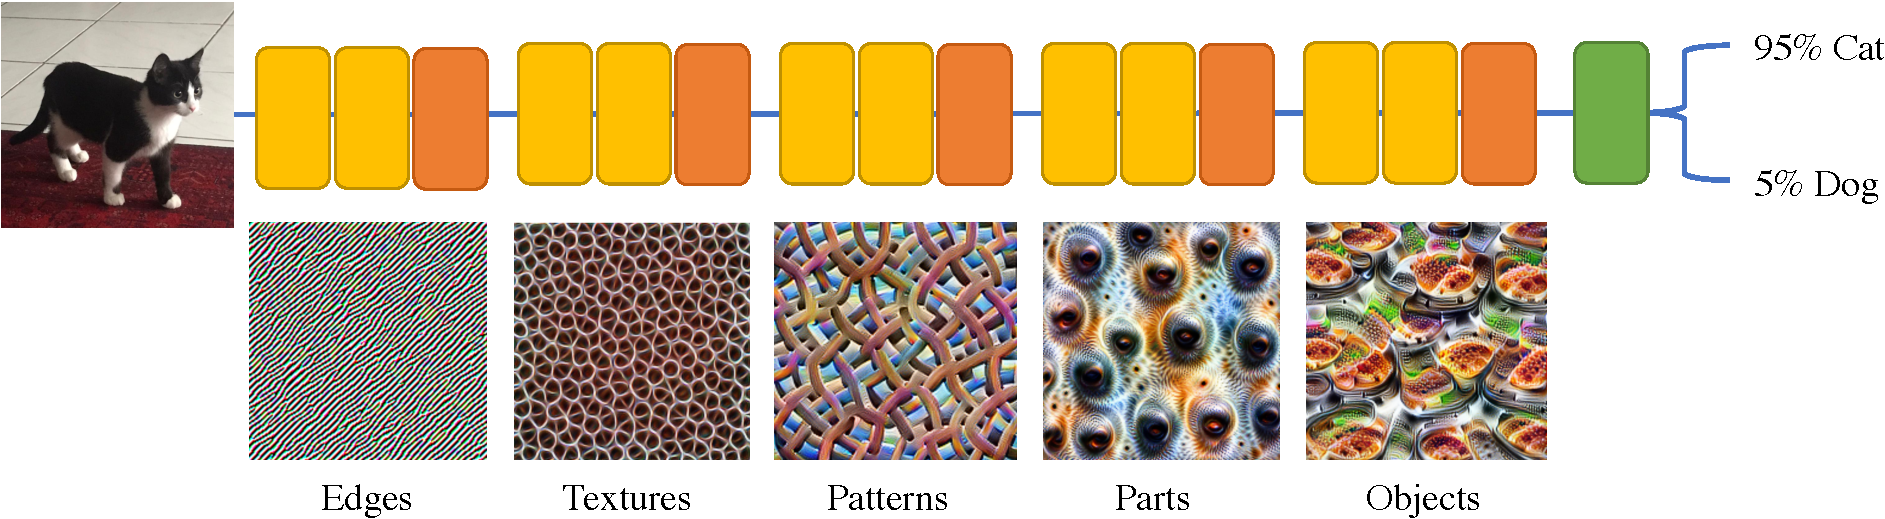
\includegraphics[width=\linewidth]{images/related/cnn.pdf}
      \end{center}
      \caption{\textbf{A Convolutional Neural Networks} extracts more complex patterns through its
            succession of convolutions. In \textcolor{orange}{orange} a convolution, in \textcolor{red}{red}
            a pooling, and in \textcolor{green}{green} the classifier. Given an image, the \ac{CNN} can assign to
            each possible class a probability, all summing to 1.
            Detected patterns taken from \cite{olah2017feature}.}
      \label{fig:related_cnn}
\end{figure}

The 2010's decade saw major improvements to \acs{CNN}, both in their architecture structure and in
their training procedure. \cite{srivastava2015highwaynet} and \cite{he2016resnet} proposed residual
connections between blocks likewise: $\vy = \vx + \sigma(\operatorname{Conv}(\vx))$. It allows
training deeper networks by enabling the gradient flows more easily up the earliest layers. This
type of connections is now quasi-ubiquitous in all \ac{DL} based architectures. Other architecture
changes include using convolutions of different kernel sizes in parallel as in Inception
\citep{szegedy2015inception}, enabling a multi-scale view of the features. These architectures are
depicted in \autoref{fig:related_resnet_inception}.

\begin{figure}[tb]
      \begin{center}
            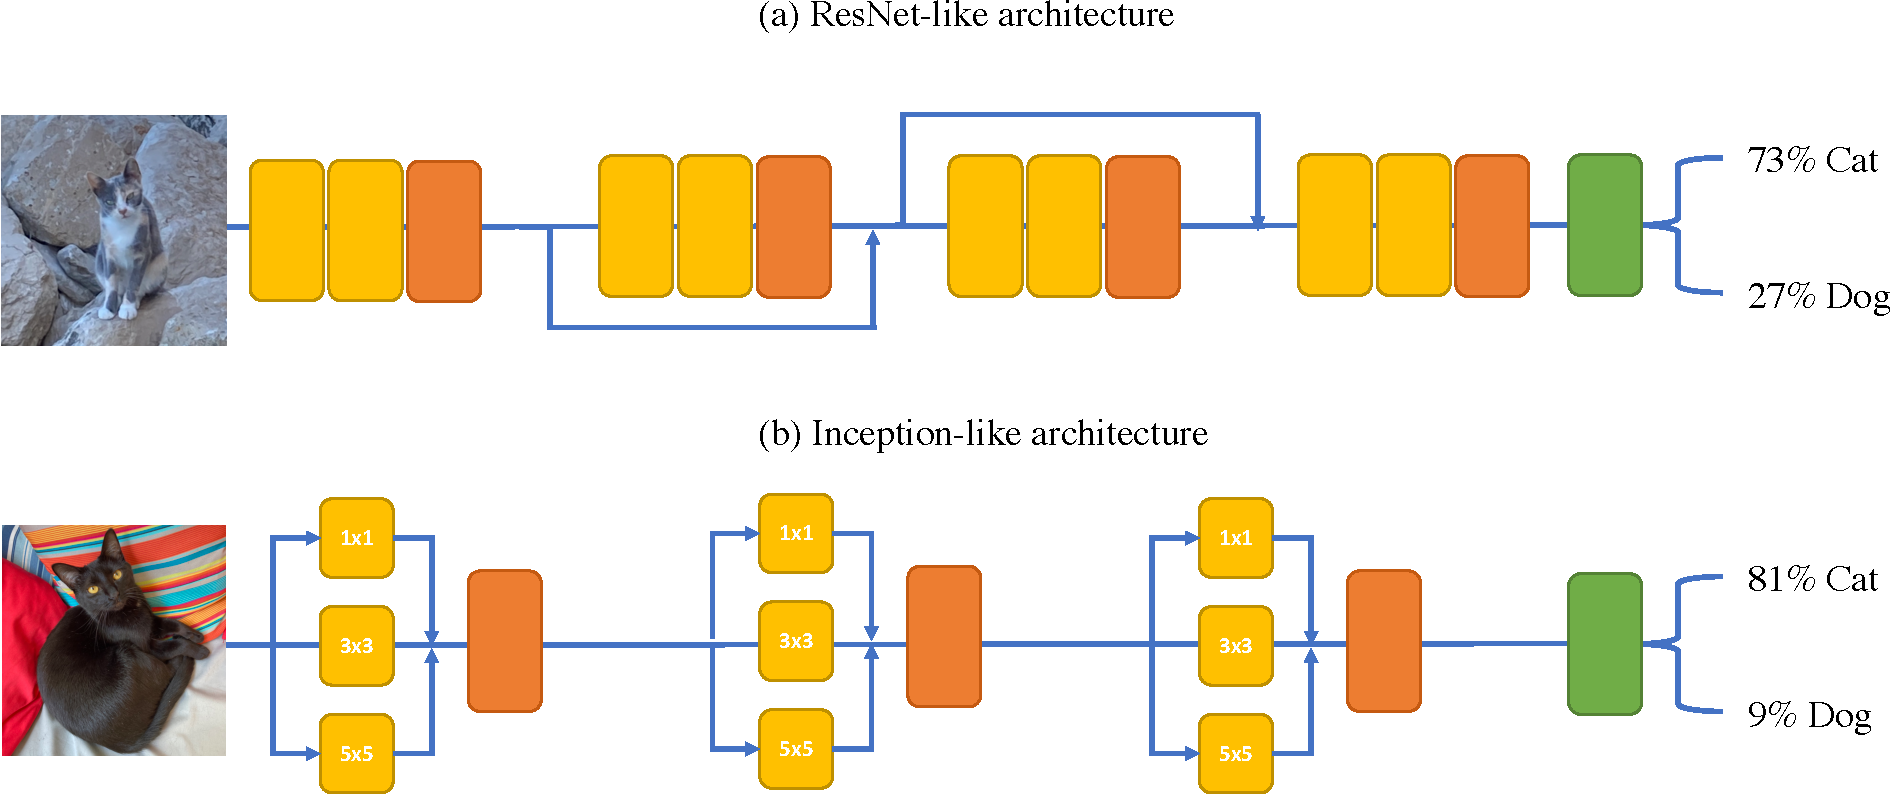
\includegraphics[width=\linewidth]{images/related/resnet_inception.pdf}
      \end{center}
      \caption{\textbf{Different CNN architectures:} \textbf{(a)} illustrates a ResNet-like architecture
            \citep{he2016resnet} where there are residual connections between blocks. Used by the vast
            majority of modern architectures, these connections help the gradient flows unchanged and
            allow training deeper networks. \textbf{(b)} showcases an Inception-like architecture where at
            the same level convolutions with different kernel sizes are used. Each detects patterns of
            different scales.}
      \label{fig:related_resnet_inception}
\end{figure}

The high performance of modern \acs{CNN} is also provided to their training procedure
\citep{wightman2019resnetstrikesback}: optimizers with adaptive learning rate such as Adam
\citep{kingma2014adam}, improved learning rate scheduling, strong data augmentations
\citep{muller2021trivialaugment,hingyi2018mixup,zhong2017erasing}, and regularizations such as
Dropout \citep{gal2016dropout} and stochastic depth \citep{gao2016stochasticdepth}.

While convolution-based neural networks dominated \acf{CV} in the 2010's decade, in the recent years
the transformer architecture gained interest: originally designed for machine translation in
\ac{NLP} \citep{vaswani2017transformer} with an encoder/decoder structure, it has been applied to
vision \citep{dosovitskiy2020vit} using a modified encoder-only structure as BERT
\citep{devlin2018bert}. A transformer's input is a sequence of ``\textit{tokens}'', which are
high-dimensional vectors. While \ac{NLP}, it used to be the learned embeddings of subwords, in
Vision it is the linear projection of patches of pixels.

\begin{figure}[tb]
      \begin{center}
            \includegraphics[width=\linewidth]{images/related/vit.png}
      \end{center}
      \caption{\textbf{The Vision Transformer (ViT):} the image is cropped without overlap and
            projected using a convolution whose stride equals the kernel size. The encoder is made of
            multiple transformer blocks. Finally, only the special learned token ``class token'' is used
            at the end, and fed to a linear classifier. Image from \cite{dosovitskiy2020vit}.}
      \label{fig:related_vit}
\end{figure}

More recently, the Transformer architecture \citep{vaswani2017transformer}, originally designed for
machine translation in \ac{NLP}, was applied to images. Using an encoder structure similar to BERT
\citep{devlin2018bert}, ViT \citep{dosovitskiy2020vit}, illustrated in \autoref{fig:related_vit},
considered patches of pixels as tokens. A special learned token, called ``class token'' is added to
the patch tokens. All the tokens are then processed through multiple transformer blocks. Each block
is made of LayerNorm \citep{ba2016layernorm}, a \ac{MHSA}, a \ac{MLP}, and residual connections.
Given a single head, the Self-Attention is:
%
\begin{equation}
      \begin{aligned}
            Q & =W_{q} \vx\,,                                                       \\
            K & =W_{k} \vx\,,                                                       \\
            V & =W_{v} \vx\,,                                                       \\
            A & =\operatorname{Softmax}\left(Q \cdot K^{T} / \sqrt{D / h}\right)\,, \\
            O & = W_{o} A V+b_{o}\,.
      \end{aligned}
      \label{sec:related_sa}
\end{equation}
%
$\vx$ are the $N$ patch tokens and the class token, of shape $(N, D)$, $D$ being the embedding
dimension. The patch tokens are linearly transformed thrice in a \textbf{Q}uery, \textbf{K}ey, and
\textbf{V}alue. An attention matrix of shape $(N, N)$ is computed from the query and the key. Its
$i^{\text{th}}$ row contains the similarity between the $i^{\text{th}}$ with all other tokens.
Finally, the multiplication between the attention matrix and the value matrix averages all tokens
according to their similarities. To extend the Self-Attention its multi-heads variation, we use
several Query/Key/Value transformations and do as many self-attentions in parallel.

\section{Continual Learning}
\label{sec:related_continual}

Usually, when training a \ac{CNN}, we assume the dataset is immutable and \textit{i.i.d.}: no new
image nor new classes will be learned. The knowledge acquired on one dataset A can be
\textit{transferred} to another dataset B with different classes using \textbf{transfer learning}
\citep{razavian2014transferlearning}. However, in that case, the new model, while being efficient on
the dataset B, cannot classify the classes of dataset A.

\textbf{Continual Learning} aims to learn a continually changing dataset without forgetting the
previous knowledge. The distribution of the dataset continually change: at each time-step, \ac{NC},
\ac{NI} from potentially new domains, or even \ac{NIC} are added to the training dataset
\cite{lomonaco2017core50}. We usually assume the test dataset evolves similarly. Continually
learning an ever-growing dataset is doable: a naive but efficient approach consist in training from
scratch a new model on the union of past and new data. However, for multiple reasons like privacy
concerns of medical data or limited storage capacity in embedded device, there is a restriction on
the amount of previous data that can be kept. In the extreme case, where a model only has access to
new data but now old data, training from scratch fails to model previous iterations' distribution.
Worse, even if the old model is kept and finetuned on the new data, it'll suffer from
\textbf{Catastrophic Forgetting} \citep{robins1995catastrophicforgetting}: new data is learned at
the expanse of old data. Multiple distribution shifts exist in Continual Learning
\citep{morenotorresa2012datasetshift,lesort2021driftanalysis}, and they have been called under various names in the
literature. I detail now the major ones, given $x$ an input sample and $y$ its label:

\begin{itemize}
      \item \textbf{Covariate shift}: when $p(x)$ changes, also known as domain incremental.
      \item \textbf{Prior shift}: when $p(y)$ changes; \ac{CIL} happens with this kind of shift.
      \item \textbf{Conceptual shift}: when $p(y | x)$ changes. Seldom covered in the literature, it
            can be found in \acf{CSS}.
\end{itemize}

In the chapter \autoref{chapter:regularization} and \autoref{chapter:dynamic}, I tackled only the
prior shift, while in \autoref{chapter:segmentation} I solved all three described shifts.

\begin{figure}[tb]
      \begin{center}
            \includegraphics[width=1.0\linewidth]{images/related/protocol}
      \end{center}
      \caption{\textbf{Training protocol for incremental learning}. At each training task we learn a
            new set of classes, and the model must retain knowledge about \textit{all} classes. The
            model is allowed a \textit{limited} memory of samples of old classes.}
      \label{fig:related_protocol}
\end{figure}

\paragraph{Class-Incremental Example} More concretely, a common benchmark in \ac{NC} setting,
commonly called \ac{CIL} is to learn the image classification CIFAR100 dataset
\citep{krizhevskycifar100} in multiple steps, each made of several new classes. \eg a model could
learn at first to classify among 10 classes, then add 10 more classes, \etc. until it has learned
all 100 classes. After each step, the model has to classify among all classes it has learned. The
\autoref{fig:related_forgetting} illustrate such continual training. The \textcolor{orange}{orange}
line displays the accuracy of a model that is re-trained from scratch at each step on all previous
classes data. This model, usually called Joint, is considered as a reasonable upper bound. The
\textcolor{blue}{blue} line on the other hand is a model that is finetuned on new classes but has no
access to previous classes. Evidently, the model's accuracy is much lower than its Joint
counterpart, because it forgets completely old classes by over-predicting new classes.

\paragraph{Single-Head \vs Multi-Heads} are the two main evaluation settings in Continual Learning
\citep{chaudhry2018riemannien_walk}. In the former setting, a model has to classify samples among
all seen classes, that could have been learned from any of the seen steps. The latter setting, on
the other hand, knows at test-time from which steps the samples come from. Thus, it only has to
classify among the limited number of classes brought by a step. This setting is closely related to
multi-tasks learning. During this thesis, I focused on the Single-Head setting because it's more
realistic as it's not always possible to know from which step a sample come from in a real-life
setting, and more challenging \citep{lesort2019regulshortcomings}.

\begin{figure}[tb]
      \begin{center}
            \includegraphics[width=0.8\linewidth]{images/related/catastrophic_forgetting.pdf}
      \end{center}
      \caption{\textbf{Training protocol for incremental learning}. At each training task we learn a
            new set of classes, and the model must retain knowledge about \textit{all} classes. The
            model is allowed a \textit{limited} memory of samples of old classes.}
      \label{fig:related_forgetting}
\end{figure}

%\paragraph{Notations} I define in \autoref{tab:related_notation} the notations used thorough this thesis.

%\chapter{Notations}

hello dfjksdhfjkhdfjkfhskjh

\begin{comment}

\begin{table}[t]
    \vspace*{-10cm}
    \centering
    \begin{tabular}{@{}l|c@{}}
        \toprule
        Total number of tasks              & $T$                                      \\
        Current task                       & $t$                                      \\
        Current classes                    & $\mcC^t$                                 \\
        Previous classes                   & $\mcC^{1:t-1}$                           \\
        Future classes                     & $\mcC^{t+1:T}$                           \\
        Cardinality of a set of classes    & $\mcN^t=\operatorname{card}(\mcC^{t})-1$ \\
        Image and label maps at task $t$   & $\vx^t$ and $\y^t$                       \\
        Feature extractor at task $t$      & $f^t(\cdot)$                             \\
        Classifier at task $t$             & $g^t(\cdot)$                             \\
        Learnable parameters at task $t$   & $\Phi^t$                                 \\
        Predicted labels                   & $\hat{y}^t$                              \\
        Intermediary features at level $l$ & $f^t_l,\,l \in \{1, \dots, L\}$          \\
        \bottomrule
    \end{tabular}
    \caption{Notations used in this paper.}
    \label{tab:related_notation}
\end{table}

\end{comment}


\subsection{Metrics for Continual Learning}
\label{sec:related_metrics}

Multiple metrics exist in Continual Learning: the most common are the \textbf{final accuracy} and
\textbf{average incremental accuracy}. The former measures the performance of the model on all tasks
at the last step. The latter measures the average of performance on all seen tasks after each new
task learned \citep{rebuffi2017icarl}. Practically, given $A_{i,t}$ the accuracy of the $i^{th}$
task after
learning the $t^{th}$ task, the final accuracy is (assuming balanced tasks):
%
\begin{equation}
      \text{Acc}_F = \frac{1}{T} \sum_{i=1}^T A_{i,T}\,,
      \label{eq:related_final_acc}
\end{equation}
%
and the average incremental accuracy:
%
\begin{equation}
      \text{Acc}_a = \frac{1}{T} \sum_{t=1}^T \frac{1}{t}  \sum_{i=1}^t A_{i,t}\,.
      \label{eq:related_avg_acc}
\end{equation}
%
Average incremental accuracy is somewhat more important than simply the final accuracy: a continual
model should be good after every step, as in a true continual setting there are no "final task".

Multiple other metrics exists \citep{diaz2018continualmetrics}, including the \textbf{backwardø and forward transfer} \citep{lopezpaz2017gem}
that measures the influence that learning a task has on the performance of respectively past and
future tasks. Another notable metric is the \textbf{forgetting} \citep{chaudhry2018riemannien_walk}
which records how much a model has lost performance-wise on a task compared to the first time it has
learned it. The interest of this metric is to be agnostic of the absolute performance of the model used.

Finally, metrics such as \textbf{speed} or used \textbf{capacity} are important: \cite{ramasesh2022scalecontinual}
recently showed that the larger a model was the lower was the forgetting.

\section{Methods to reduce forgetting}
\label{sec:related_methods}

Multiple approaches exist to reduce forgetting in Continual Learning. The major ones are
review of old data (\autoref{sec:related_rehearsal}), regularizations constraining the model's
behavior (\autoref{sec:related_regul}), and structural adaptations \autoref{sec:related_structural}.
In the \autoref{chapter:regularization} and \autoref{chapter:segmentation} both the first and second
approaches are considered. In the \autoref{chapter:dynamic}, the first and third approach are evaluated.

\subsection{Rehearsal}
\label{sec:related_rehearsal}

The most efficient method to reduce forgetting is \textbf{rehearsal learning} where old samples will
be seen alongside the new samples. The amount of old samples stored is extremely limited otherwise
it would defect the purpose of continual learning. \autoref{fig:related_protocol} illustrates how
rehearsal learning happens in Continual Learning. During the first step, a model is trained on all
available samples. Then, it stores a limited amount of those in a \textit{memory}. During the second
step, the model has access to new samples but also all samples stored in the memory. In
Class-Incremental, an equal amount of samples per class is stored in memory. Nevertheless, there are
two major approaches to determine this amount: \cite{rebuffi2017icarl} proposed to fully use a
memory of size $\mcM$ among all $\mcC$, while \cite{hou2019ucir} instead kept fixed the amount of
samples stored per class to $\nicefrac{\mcM}{|\mcC|}$.

\paragraph{Herding} is the action of choosing which samples per class to store in the rehearsal
memory. The most naive herding method is to sample randomly images. Despite its simplicity, it's
quite competitive with more complex method \citep{castro2018end_to_end_inc_learn}, echoing similar
results in \ac{AL} \citep{gal2017activelearning}. Other herding methods include fetching samples
close to the class mean in the feature space \citep{castro2018end_to_end_inc_learn} or close to an
incremental barycenter \citep{rebuffi2017icarl}.

\paragraph{Sampling} is an important but yet fewly investigated topic in Continual Learning. Most
models mix all memory samples with new samples without any under- or over-sampling.
\cite{castro2018end_to_end_inc_learn} propose to finetune for a few epochs, after training on a new
step, on a balanced set of old and new classes samples. \cite{chaudhry2019tinyepisodicmemories}
oversample tiny memory with as low as one sample per class, and show, in the context of Online
Learning (\autoref{sec:related_online_learning}), that continual models still don't overfit. In the
same context, \cite{aljundi2019maximallyinterfered} proposed to over-sample the memory examples with
highest losses. In an imbalanced situation for Continual Learning, over- and under-sampling can be
applied depending on the amount of samples per classes \citep{kim2020imbalancedcontinual}.

\paragraph{Efficient Storing} is important for rehearsal learning: a bigger rehearsal memory leads
invariably to less forgetting \citep{douillard2020podnet}. Thus, several works considered how more
samples could be stored given the same memory size: \cite{hayes2020remind} compress intermediate
features of memory samples with a lossless compression algorithm.
\cite{iscen2020incrementalfeatureadaptation} also store features but modify them through the
training to handle the inherent internal covariate shift. \cite{douillard2021objectrehearsal}, in
the context of segmentation, store only non-regular patches of zones of interest instead of storing
the whole, large, images.

\paragraph{Pseudo-rehearsal} doesn't need to store samples, but instead generates pseudo-samples for
rehearsal \citep{lesort2019generative}. The generation can be done with auto-encoders from
intermediate features \citep{kemker2018fearnet,ayub2021eec} or use \ac{GAN}
\citep{shin2017deep_generative_replay}. Those methods unfortunately have several drawbacks: they
struggle to scale to large images, the generator size may be superior to a classic rehearsal memory
size which would defeat the goal of using less storage, and finally the generator may itself suffer
from catastrophic forgetting. \cite{liu2020mnemonics} propose instead a method halfway between
rehearsal and pseudo-rehearsal: the authors sample randomly real images, and then during continual
training, slightly modify them via bi-level optimization to minimize forgetting.


\begin{figure}[tb]
      \begin{center}
            \includegraphics[width=1.0\linewidth]{images/related/rehearsal}
      \end{center}
      \caption{\textbf{Training protocol for incremental learning}. At each training task we learn a
            new set of classes, and the model must retain knowledge about \textit{all} classes. The
            model is allowed a \textit{limited} memory of samples of old classes.}
      \label{fig:related_protocol}
\end{figure}

\autoref{fig:related_protocol}


\subsection{Regularization-based Approaches}
\label{sec:related_regul}


\begin{figure}[tb]
      \begin{center}
            \includegraphics[width=1.0\linewidth]{images/related/constraints}
      \end{center}
      \caption{\textbf{Training protocol for incremental learning}. At each training task we learn a
            new set of classes, and the model must retain knowledge about \textit{all} classes. The
            model is allowed a \textit{limited} memory of samples of old classes.}
      \label{fig:related_protocol}
\end{figure}

A common and efficient way to reduce forgetting, is to minimize the difference in behavior between
the old and new models as illustrated in \autoref{fig:related_regul}. These constraints can be
expressed through various forms as described below.

\subsubsection{Weight-based}
\label{sec:related_regul_weight}


The most straightforward way to avoid completely forgetting, is that the old and new
models are identical. While the model would be \textit{rigid} (no forgetting), it is also not
\textit{plastic} at all, and thus cannot learn any new tasks. Thus, a line of research proposed to
constrain only a portion of the neurons:
%
\begin{equation}
      \mcL(\theta) = \mcL_\mcT(\theta) + \lambda \sum_i \Omega_i (\theta_i - \theta_i^*)^2\,,
      \label{eq:related_weight_constraint}
\end{equation}
%
where $\mcL_\mcT(\theta)$ is the loss of the current task (\eg the cross-entropy), $\theta_i$ and
$\theta_i^*$ respectively the $i^\text{th}$ neuron of the current and previous model, and $\Omega_i$
a neuron-wise importance factor. The intuition is that important neuron for $\mcT-1$ shouldn't
change, while the others can be adapted to fit the new task $\mcT$.

\cite{kirkpatrick2017ewc}, followed by
\cite{zenke2017synaptic_intelligence} and \cite{chaudhry2018riemannien_walk}
proposed to use the diagonal Fisher information matrix as importance factors.
\cite{aljundi2018MemoryAwareSynapses} instead used the sensitivity of the model when
small perturbations are added to the neurons to measure their importance.

However, it's worth remarking that weight-based constraints are usually limited to the multi-heads
setting where a task identifier is available at test time. \cite{lesort2019regulshortcomings} showed
that in the more realistic single-head setting, they barely reduce forgetting and were significantly
outperformed by rehearsal-based methods.

\subsubsection{Gradient-Based}
\label{sec:related_regul_gradient}

\begin{figure}[tb]
      \begin{center}
            \includegraphics[width=1.0\linewidth]{images/related/gem.pdf}
      \end{center}
      \caption{\textbf{GEM's gradient constraint} forcing updates to be in the same direction as the
            gradient \wrt old samples.}
      \label{fig:related_gem}
\end{figure}

\cite{lopezpaz2017gem} proposed the GEM model which combines a constraint on the gradients and
rehearsal learning. The algorithm requires that the loss on a given stored sample must not increase
despite the model learning new classes. The authors, given a locality assumption, rewrite this
formulation as enforcing that the gradient of a new sample ($g$) to be in the same \textit{direction} as
the gradient of a stored old sample ($g_i$):
%
\begin{equation}
      \langle g,\, g_i\rangle \ge 0,\, \text{for all} i \in \mcM
\end{equation}
%
With $\mcM$ the rehearsal memory. If the constraint is violated, the new gradient $g$ is projected
to the closest in L2 norm gradient that satisfies the angle constraint by minimizing a quadratic
program. The constraint is illustrated in \autoref{fig:related_gem}. The drawback of this method is
the computational cost that can grow prohibitively when the memory is too large.
\cite{chaudhry2019AGEM} proposed Averaged-GEM to speed up GEM: the author don't constraint the
gradient of individual memory samples but only the average of all memory samples.
\cite{aljundi2019gradientselection} also improved GEM's speed by selecting only a subset of the
memory samples that maximize the feasible region.

Differently, but still constraining the gradients: \cite{farajtabar2020ogd}'s OGD forces the gradients of
task $t$ to be orthogonal to gradients of task $t-1$. They use the Gram-Schmidt procedure to
orthogonalize the new gradients, allowing updates for the new task that minimally interfere with the
performance of old tasks. \cite{saha2021gpm}'s GPM does likewise but using instead a k-rank
approximation of the SVD of the representation matrix.


\subsubsection{Output-based}
\label{sec:related_regul_output}

Finally, the majority of Continual model that are benchmarked on large datasets (\eg ImageNet
\citep{deng2009imagenet}, Pascal VOC \citep{everingham2015pascalvoc}) use a combination of rehearsal
learning (\autoref{sec:related_rehearsal}) and constraints on the model's outputs.

LwF \cite{li2018lwf} and iCaRL applied the \ac{KD} \cite{hinton2015knowledge_distillation} on the
model's probabilities. It usually consists in minimizing the \ac{KL} between the probabilities
of the old and new models:
%
\begin{equation}
      \mcL_\text{KD} = \operatorname{KL}(\operatorname{softmax}(\frac{\tilde{y}^{t-1}}{\tau}) \Vert \operatorname{softmax}(\frac{\tilde{y}^t}{\tau})\,,
\end{equation}
%
where $\tilde{y}^{t-1}$ and $\tilde{y}^{t}$ are respectively the logits of the old and new model,
and $\tau$ a \textit{temperature} to soften the probabilities in order to give more importance to
the \textit{dark knowledge} of \cite{hinton2015knowledge_distillation}. Note that in the context of
Class-Incremental, the new model predicts more classes than the old model, therefore the \ac{KL} is
only applied on the logits common to both the old and the new models. The \ac{KD} is sometimes also
defined as the binary cross-entropy between the sigmoid-activated logits.

Constraining the probabilities is now so ubiquitous that most models include it in their base
losses. On the other hand, a few models considered constraining intermediate outputs. MK2D
\citep{peng2019m2kd} uses the \ac{KD} from both the final classifier and an auxilliary classifier
similarly to the Inception network \citep{szegedy2015inception}. \cite{hou2019ucir} maximizes the
cosine similarity between the embeddings produced by the \ac{GAP}.
\cite{dhar2019learning_without_memorizing_gradcam} minimizes the L1 distance between the attention
maps produced by GradCam \citep{selvaraju2017gradcam}. Drawing inspiration from the model
compression litterature \cite{zagoruyko2016distillation_attention}, \cite{douillard2020podnet}
proposed to constraint instead the statistics of all intermediate features of the \ac{ConvNet}. This
constraint was later expanded to incorporate multiscale information \cite{douillard2020plop}.

\subsection{Structural Strategies}
\label{sec:related_structural}

\begin{figure}[tb]
      \begin{center}
            \includegraphics[width=0.6\linewidth]{images/related/subnetworks.pdf}
      \end{center}
      \caption{\textbf{Task-specific subnetworks} that can be uncovered with a sparsity loss or
            learned masking.}
      \label{fig:related_subnetwork}
\end{figure}

Multiple works have also proposed to adopt dynamic strategies where the configuration of the neural
network is different for each task to learn.

\paragraph{Subnetworks} The Lottery Ticket Hypothesis \citep{frankle2019lottery_ticket} states that
subnetworks, made of a fraction of the neurons and connections of a larger network, can reach
excellent performance. Several Continual Learning models have exploited that property by using a
subnetwork per task. Those subnetworks can be uncovered via genetic algorithms
\citep{fernando2017path_net}, via induced L1 sparsity \citep{golkar2019neural_pruning}, or even
learned masked \cite{serra2018hat,hung2019cpg}. Usually, these methods require a task identifier at
test-time in order to select the right subnetwork (see \textit{multi-heads} in
\autoref{sec:related_continual}). Later, \cite{wortsman2020supermasks} proposed to infer the task
identifier by selecting the subnetwork with the lowest entropy. This subnetwork-based approach is
illustrated in \autoref{fig:related_subnetwork}.

\paragraph{Expandable Networks} A neural network can also be expanded thorough its continual
training to accommodate the growing amount of tasks to solve. First, \cite{rusu2016progressive}
proposed to have one network per task, where the $i^{\text{th}}$ network would depend both on the
input and all previous networks' intermediate features. Unfortunately, the memory consumption is
quickly prohibitive with many tasks. Following works have proposed to only add blocks of parameters,
and only when deemed necessary
\citep{hung2019cpg,veniat2021mntdp,ostapenko2021localmodulecomposition}.

\paragraph{Task Conditioning} Rather than adding many new parameters, it's also possible to only add
a few parameters that will adapt the existing network \citep{rebuffi2017visualadapters}:
\cite{wen2020batchensemble} and \cite{sun2019metatransfer} proposed to share most of the weights
across tasks, but have task-specific weights that directly modify the shared weights.

\paragraph{Mixture-of-Experts} Mixture of experts \citep{masoudnia2014mixture} have also been
proposed, where multiple experts combine their decision. \cite{aljundi2017experts} learn a gating
system to use the right task-specific expert. \cite{yan2021der} and \cite{li2021preserve} proposed
to have a \ac{ConvNet} per task, and to concatenate their output embeddings to be fed to a single
classifier. To avoid parameters explosion, they aggressively prune each \ac{ConvNet}.

\paragraph{Classifier Correction} Forgetting happen in both the feature extractor and the
classifier. Previously described rehearsal and regularization methods try to reduce it in both
places. On the other hand, multiple works focused solely on the classifier. They remarked that in
\acf{CIL}, the classifier is miscalibrated \citep{guo2017miscalibration} where the model
over-predicts new classes to the detriment of old classes. \cite{belouadah2019il2m} compensate the
bias towards new classes by rectifying predictions of past classes using their recorded accuracies
and confidences. \cite{wu2019bias_correction} learn a linear model on validation data to recalibrate
the logits of the new classes. \cite{zhao2020weightalignement} normalizes the norm of the classifier
weights associated to new classes so that their average norm becomes the same as that for old
classes. \cite{hou2019ucir}, aims for a similar result, by replacing the dot product in the
classifier by a cosine similarity, resulting in classifier weights of unit norm for all.


\cleardoublepage
\let\leftmark=\oldleftmark

\acresetall
\chapter{Feature-based Regularizations}
\label{chapter:regularization}

%\newcommand{\mcL}{\mathcal{L}}
%\newcommand{\vx}{\mathbf{x}}
%\newcommand{\vh}{\mathbf{h}}
%\newcommand{\vy}{\mathbf{y}}
\newcommand{\tableindent}{\,\,\,\,}
\newcommand{\vt}{\mathbf{t}}
%\newcommand{\vyh}{\hat\vy}
\newcommand{\pp}{\,\textit{p.p}}
\newcommand{\std}{$\pm\,$}
\newcommand{\clf}{\textit{clf}}
\newcommand{\gray}[1]{{\color{darkgray}#1}}


\begin{chapabstract}
    Regularization-based methods are powerful approaches to reduce catastrophic
    forgetting, especially in challenging setting such as \ac{CIL} with single-head
    where task identity is not known at test-time. However, they often consider
    only constraining the final probability predictions of the network which falls
    short to forgetting when faced to large amount of tasks. \\
    In this chapter, we propose two methods exploiting explicitly the intermediate
    features to reduce forgetting. The first approach, nicknamed PODNet, aims to
    constrain similar statistics to avoid a representation drift at all levels
    of the network. We show that it scales particularly well on extreme scenarios
    where classes are learned one by one for a long succession of iterations.
    The second approach, named Ghost, pre-emptively reserves
    capacity for future ---yet to be seen--- classes avoiding forgetting before
    it even happens. We pinpoint those classes locations in the representation
    space by estimating their future positions by drawing inspiration from the
    \ac{ZSL} literature.

    The work in this section has led to a publication to a conference paper (PODNet) and a workshop
    paper (Ghost):

    \begin{itemize}
        \item \fullcite{douillard2020podnet}
        \item \fullcite{douillard2020ghost}
    \end{itemize}

\end{chapabstract}
\newpage

\minitoc
\chapterwithfigures{\nameref*{chapter:regularization}}
\chapterwithtables{\nameref*{chapter:regularization}}

\ifthenelse{\boolean{skipRegul}}{\endinput}{}

\section{Introduction}

\ac{CIL}, where each task brings new classes, is among the most challenging setting of \ac{CL}. When
evaluated in single-head, where the task identity is not known at test-time, the majority of the
methods rely on rehearsal learning where a limited amount of old data is replayed. Furthermore, it
is often combined to regularizations that aim to limit forgetting. These regularizations are often a
knowledge distillation \citep{hinton2015knowledge_distillation} that enforces similar probabilities
between the old and current model. First introduced by LwF \citep{li2018lwf}, it has then be used by
multiple seminal papers including iCaRL \citep{rebuffi2017icarl} and WA
\citep{zhao2020weightalignement}. I propose in this chapter two proposed regularization methods to
reduce forgetting. The first one, introduced in \ac{PODNet} \citep{douillard2020podnet}, aims to
regularize the statistics shift at the intermediate feature-level to reduce significantly
catastrophic forgetting. The second one, nicknamed Ghost \citep{douillard2020ghost}, on the other
hand, avoid pre-emptively forgetting by regularizing the feature space at locations where future
classes are estimated to arrive to.

\section{PODNet: reducing forgetting via intermediate feature statistics}

Lifelong machine
learning~\citep{robins1995catastrophicforgetting,french1999catastrophicforgetting,thrun1998lifelonglearning}
focuses on models that accumulate and refine knowledge over large timespans. Incremental learning
--\,the ability to aggregate different learning objectives seen over time into a coherent whole\,--
is paramount to those models. To achieve incremental learning, models must fight
\textit{catastrophic
    forgetting}~\citep{robins1995catastrophicforgetting,french1999catastrophicforgetting} of previous
knowledge. Lifelong and incremental learning have attracted much attention in the past few years,
but existing works still struggle to preserve acquired knowledge over many cycles of short
incremental learning steps.

We will focus on image classifiers, which are ordinarily trained once on a fixed set of classes. In
\textit{incremental learning}, however, the classifier must learn the classes by steps, in training
cycles called \textit{tasks}. At each task, we expose the classifier to a new set of classes.
Incremental learning would reduce trivially to ordinary classification if we were allowed to store
all training samples, but we are imposed a limited \textit{memory}: a maximum number of samples for
previously learned classes. This limitation is motivated by practical applications, in which privacy
issues, or storage and computing limitations prevent us from simply retraining the entire model for
each new task~\citep{li2018lwf,lomonaco2017core50}. Furthermore, incremental learning is different
from transfer learning in that we aim to have good performance in both old and new classes.

To overcome catastrophic forgetting, different approaches have been proposed: reusing a limited
amount of previous training data~\citep{rebuffi2017icarl,castro2018end_to_end_inc_learn}; learning
to generate the training data~\citep{kemker2018fearnet,shin2017deep_generative_replay}; extending
the architecture for new phases of
data~\citep{yoon2018dynamically_expandable_networks,li2019learning_to_grow}; using a sub-network for
each phase~\citep{fernando2017path_net,golkar2019neural_pruning}; or constraining the model
divergence as it
evolves~\citep{kirkpatrick2017ewc,lopezpaz2017gem,aljundi2018MemoryAwareSynapses,li2018lwf,rebuffi2017icarl,castro2018end_to_end_inc_learn}.


In this work, we propose PODNet, approaching incremental learning as representation learning, with a
distillation loss that constrains the evolution of the representation. By carefully balancing the
compromise between remembering the old classes and learning new ones, we learn a representation that
fights catastrophic forgetting, remaining stable over long runs of small incremental tasks. Our
model innovates on existing art with (1) an \textit{efficient spatial-based} distillation-loss
applied \textit{throughout the model}; and (2) as a refinement, a representation comprising multiple
proxy vectors for each class, resulting in a more flexible representation.

In this paper, we first present the existing state of the art (\autoref{sec:related_work}), which we
close by detailing our contributions. We then describe our model (\autoref{sec:model}), and evaluate
it in an extensive set of experiments (\autoref{sec:expes}) on CIFAR100, ImageNet100, and
ImageNet1000, including ablation studies assessing each contribution, and extensive comparisons with
existing methods.

\section{Related Work}
\label{sec:related_work}

To approach the problem of incremental learning, consider a single incremental task: one has a
classifier already trained over a set of old classes and must adapt it to learn a set of new
classes. To perform that single task, we will consider: (1) the data/class representation model; (2)
the set of constraints to prevent catastrophic forgetting; (3) the experimental context (including
the constraints over the memory for previous training data) for which to design the model.

\paragraph{Data/class representation model} Representation learning was already implicitly present
in iCaRL~\citep{rebuffi2017icarl}: it introduced the Nearest Mean Exemplars (NME) strategy which
averages the outputs of the deep convolutional network to create a single proxy feature vector per
class that are then used by a nearest-neighbor classifier predict the final classes. Hou et
al.~\citep{hou2019ucir} adopted this method and also introduced another, named CNN, which uses the
output class probabilities to classify incoming samples, freezing (during training) the classifier
weights associated with old classes, and then fine-tuning them on an under-sampled dataset.

Hou et al.~\citep{hou2019ucir}, in the method called here UCIR, made representation learning
explicit, by noticing that the limited memory imposed a severe imbalance on the training samples
available for the old and for the new classes. To overcome that difficulty, they designed a
metric-learning model instead of a classification model. That strategy is often used in few-shot
learning~\citep{gidaris2018fewshot_wo_forgetting} because of its robustness to few data. Because
classical metric architectures require special training sampling (e.g., semi-hard sampling for
triplets), Hou et al. chose instead to redesign the classifier's last layer of their model to use
the cosine similarity~\citep{luo2018cosine_classifier}.

\paragraph{Model constraints to prevent catastrophic forgetting} Constraining the model's evolution
to prevent forgetting is a fruitful idea proposed by several
methods~\citep{kirkpatrick2017ewc,lopezpaz2017gem,aljundi2018MemoryAwareSynapses,li2018lwf,rebuffi2017icarl,castro2018end_to_end_inc_learn}.

%A loss function may constrain the weights directly~\citep{ewc}, the gradients~\citep{gem}, or the
%output probabilities~\citep{lwf}.
Preventing the model's parameters from diverging too much forces it to remember the old classes, but
care must be taken to still allow it to learn the new ones. We call this balance the
\textit{rigidity-plasticity trade-off}.

Existing art on knowledge distillation/compression~\citep{hinton2015knowledge_distillation} was an
important source of inspiration for constraints on models. The goal is to distill a large trained
model (called teacher) into a new smaller model (called student). The distillation loss forces the
features of the student to approach those of its teacher. In our case, the student is the current
model and the teacher---with same capacity-- is its version at the previous task. Zagoruyko and
Komodakis~\citep{komodakis2017attention_residual_distillation} investigated attention-based
distillation for image classifiers, by pooling the intermediate features of convolutional networks
into attention maps, then used in their distillation losses. Li and Hoiem~\citep{li2018lwf} —-\,and
several authors after
them~\citep{rebuffi2017icarl,castro2018end_to_end_inc_learn,wu2019bias_correction}\,—- used a binary
cross-entropy between the output probabilities by the models. Hou et al.~\citep{hou2019ucir}, used
instead \textit{Less-Forget}, a cosine-similarity constraint on the flat feature embeddings after
the global average pooling. Dhar et al.~\citep{dhar2019learning_without_memorizing_gradcam} proposed
to constrain the gradient-based attentions generated by GradCam~\citep{selvaraju2017gradcam}, a
visualization method. Wu et al.~\citep{wu2019bias_correction} proposed BiC, an algorithm oriented
towards large-scale datasets, which employs a small linear model learned on validation data to
recalibrate the output probabilities before applying a distillation loss.

\paragraph{Experimental context} A critical component of incremental learning is the convention used
for the memory storing samples of previous data. An usual convention is to consider a fixed amount
of samples allowed in that memory, as illustrated in \autoref{fig:protocol}.

Still, there are two experimental protocols for such fixed-sample convention: we may either use the
memory budget at will ($M_\mathrm{total}$), or add a constraint on the number of samples per class
for the old classes ($M_\mathrm{per}$). When $M_\mathrm{total}=M_\mathrm{per}\times$\textit{\# of
    classes}, both settings have equivalent \textit{final} memory size, but the latter, that we adopt,
is much more challenging since early tasks cannot benefit from the full memory size. \textit{The
    granularity of the increments} is another critical element: with a fixed number of classes,
increasing the number of tasks decreases the number of classes per task. More tasks imply stronger
forgetting of the earliest classes, and pushing that number creates a challenging protocol, so far
unexplored by existing art. Hou et al. evaluate at most 10 tasks on CIFAR100, while we propose as
much as 50 tasks.

Finally, to score the experiments, Rebuffi et al.~\citep{rebuffi2017icarl} proposed a global metric
that they called \textbf{average incremental accuracy}, taking into account the entire history of
the run, averaging the accuracy at the end of each task (including the first).
%\textit{The granularity of the increments} is another critical element. Hou et al.~\citep{ucir}
%introduced a protocol where one starts by training the models on half the classes and then divides
%the remaining classes equally among the remaining tasks. For example for 100 classes and 5 tasks,
%one would have a starting task with 50 classes and perform 5 additional tasks of 10 classes.
%Increasing the number of tasks decreases the number of classes per task. A high number of task is a
%challenging protocol and yet so far unexplored: Hou et al. evaluates itself with at most 10 tasks
%on CIFAR100 while we push this boundary to 50 tasks.

\begin{figure}[tb]
    \begin{center}
        \includegraphics[width=0.8\linewidth]{images/podnet/protocol}
    \end{center}
    \caption{\textbf{Training protocol for incremental learning}. At each training task we learn a
        new set of classes, and the model must retain knowledge about \textit{all} classes. The
        model is allowed a \textit{limited} memory of samples of old classes.}
    \label{fig:protocol}
\end{figure}

\paragraph{Contributions} As seen, associating representation learning to model constraints is a
particularly fruitful idea for incremental learning, but requires carefully balancing the goals of
rigidity (to avoid catastrophic forgetting) and plasticity (to learn new classes).

Employing a distillation-based loss to constrain the evolution of the representation has also
resulted in leading
results~\citep{hou2019ucir,wu2019bias_correction,peng2019m2kd,dhar2019learning_without_memorizing_gradcam}.
Our model improves existing art by employing a \textit{novel and efficient spatial-based}
distillation loss, which we are able to apply \textit{throughout the model}.

Implicit or explicit proxy vectors representing each class inside the models have lead to state of
the art results~\citep{rebuffi2017icarl,hou2019ucir}. Our model extends that idea allowing for
\textit{multiple proxy vectors} per class, resulting in a more flexible representation.


Formally, we learn the model in $T$ \textit{tasks}, task $t$ comprising a set of new classes
$C^t_N$, and a set of old classes $C^t_O$, and aiming at classifying all seen classes $C^t_O \cup
    C^t_N$. Between tasks, the new set $C^t_O$ will be set to $C^{t-1}_O \cup C^{t-1}_N$, but the amount
of training samples from $C^t_O$ (called \textit{memory}) is constrained to exactly $M_\mathrm{per}$
samples per class, while all training samples in the dataset are allowed for the classes in $C^t_N$.

\subsection{Model}
\label{sec:podnet_model}

Our base model is a deep convolutional network $\vyh = g(f(\vx))$, where $\vx$ is the input image,
$\mathbf{y}$ is the output vector of class probabilities, $\vh = f(\vx)$ is the ``feature
extraction'' part of the network (all layers up to the next-to-last), $\vyh = g(\vh)$ is the final
classification layer, and $\vh$ is the final embedding of the network before classification
(\autoref{fig:model}). The superscript $t$ denotes the model learned at task $t$:$f^{t}$, $g^{t}$,
$\vh^{t}$, etc.

Our strategy is made of two keys components: a distillation loss applied at the intermediate
feature-level, and a local-similarity classifier.

\subsubsection{POD: Pooled Outputs Distillation loss}
\label{sec:pod}

Constraining the evolution of the weights is crucial to reduce forgetting. Each new task $t$ learns
a new (student) model, whose weights are not only initialized with those of the previous (teacher)
model, but also constrained by a distillation loss. That loss must be carefully balanced to prevent
forgetting (rigidity), while allowing the learning of new classes (plasticity).

To this goal, we propose a set of constraints we call \textbf{Pooled Outputs Distillation (POD)},
applied not only over the final embedding output by $\vh^{t}=f^{t}(\vx)$, but also over the output
of its intermediate layers $\vh^{t}_\ell=f^{t}_\ell(\vx)$ (where by notation overloading
$f^{t}_\ell(\vx)\equiv f^{t}_\ell\circ\ldots\circ f^{t}_1(\vx)$, and thus $f^{t}(\vx)\equiv
    f^{t}_L\ldots\circ f^{t}_\ell\circ\ldots f^{t}_1(\vx)$).

The convolutional layers of the network output tensors $\vh^{t}_{\ell}$ with components
$\vh^{t}_{\ell,c,w,h}$, where $c$ stands for channel (filter), and $w\times h$ for column and row of
the spatial coordinates. The loss used by POD may pool (sum over) one or several of those indexes,
more aggressive poolings (\autoref{fig:pooling}) providing more freedom, and thus, plasticity: the
lowest possible plasticity imposes an exact similarity between the previous and current model while
higher plasticity relaxes the similarity definition.

Pooling is an important operation in Computer Vision, with a strong theoretical motivation. In the
past, pooling has been introduced to obtain invariant
representations~\citep{lowe1999sift,lazbnik2006spatial_pyramid_matching}. Here, the justification is
similar, but the goal is different: as we will see, the pooled indexes are aggregated in the
proposed loss, allowing \textit{plasticity}. Instead of the model acquiring invariance to the input
image, the desired loss acquires invariance to model evolution, and thus, representation.
%
The proposed pooling-based formalism has two advantages: first, it organizes disparately proposed
distillation losses into a neat, general formalism. Second, as we will see, it allowed us to propose
novel distillation losses, with better plasticity-rigidity compromises. Those topics are explored
next.

\begin{figure}[tb]
    \begin{center}
        \includegraphics[width=0.90\linewidth]{images/podnet/pooling}
    \end{center}
    \caption{\textbf{Different possible poolings}. The output from a convolutional layer
        $\vh^{t}_{\ell,c,w,h}$ may be pooled (summed over) one or more axes. The resulting loss
        considers only the pooled activations instead of the individual components, allowing more
        plasticity across the pooled axes.}
    \label{fig:pooling}
\end{figure}

\paragraph{Pooling of convolutional outputs} As explained before, POD constrains the output of each
intermediate convolutional layer $\vh^{t}_{\ell,c,w,h} = f^{t}_\ell(\cdot)$ (in practice, each stage
of a ResNet~\citep{he2016resnet}). As a reminder, $c$ is the channel and $w\times h$ are the spatial
coordinates. All POD variants use the Euclidean distance of $\ell^2$-normalize tensors, here noted
as $\left\Vert\cdot-\cdot\right\Vert$. They differ on the type of pooling applied before that
distance is computed.
%
On one extreme, one can apply no pooling at all, resulting in the most strict loss, the most rigid
constrains, and the lowest plasticity:
%
\begin{equation}
    \mcL_{\text{POD-pixel}}(\vh^{t-1}_\ell, \vh^t_\ell) = \sum_{c=1}^C \sum_{w=1}^{W} \sum_{h=1}^{H} \left\Vert \vh^{t-1}_{\ell,c,w,h} - \vh^t_{\ell,c,w,h} \right\Vert^2\label{eq:pod_pixel}\,.
\end{equation}
%
By pooling the channels, one preserves only the spatial coordinates, resulting in a more permissive
loss, allowing the activations to reorganize across the channels, but penalizing global changes of
those activations across the space,
%
\begin{equation}
    \mcL_{\text{POD-channel}}(\vh^{t-1}_\ell, \vh^t_\ell)  = \sum_{w=1}^{W} \sum_{h=1}^{H} \left\Vert \sum_{c=1}^C \vh^{t-1}_{\ell,c,w,h} - \sum_{c=1}^C \vh^{t}_{\ell,c,w,h} \right\Vert^2\label{eq:pod_channel}\,;
\end{equation}
%
or, contrarily, by pooling the space (equivalent, up to a factor, to a Global Average Pooling), one
preserves \textit{only} the channels:
%
\begin{equation}
    \mcL_{\text{POD-gap}}(\vh^{t-1}_\ell, \vh^t_\ell) = \sum_{c=1}^{C} \left\Vert \sum_{w=1}^{W} \sum_{h=1}^H \vh^{t-1}_{\ell,c,w,h} - \sum_{w=1}^{W} \sum_{h=1}^H \vh^{t}_{\ell,c,w,h} \right\Vert^2\label{eq:pod_gap}\,.
\end{equation}
%

Note that the only difference between the variants is in the position of the summation. For example,
contrast equations \autoref{eq:pod_pixel} and \ref{eq:pod_channel}: in the former the differences
are computed between activation pixels, and then totaled; in the latter, first the channel axis is
flattened, then the differences are computed, resulting in a more permissive loss.

We can trade a little plasticity for rigidity, with less aggressive pooling by aggregating
statistics across just one of the spatial dimensions:
%
\begin{equation}
    \mcL_{\text{POD-width}}(\vh^{t-1}_\ell, \vh^t_\ell)  = \sum_{c=1}^{C} \sum_{h=1}^{H} \left\Vert \sum_{w=1}^W \vh^{t-1}_{\ell,c,w,h} - \sum_{w=1}^W \vh^{t}_{\ell,c,w,h} \right\Vert^2\label{eq:pod_width}\,;
\end{equation}
%
or, likewise, for the vertical dimension, resulting in POD-height. Each of those variants measure
the distribution of activation pixels across their respective axis. These two complementary
intermediate statistics can be further combined together:
%
\begin{equation}
    \mcL_{\text{POD-spatial}}(\vh^{t-1}_\ell, \vh^t_\ell) = \mcL_{\text{POD-width}}(\vh^{t-1}_\ell, \vh^t_\ell) + \mcL_{\text{POD-height}}(\vh^{t-1}_\ell, \vh^t_\ell)\,.
\end{equation}
%
$\mcL_{\text{POD-spatial}}$ is minimal when the average statistics over the dataset, on both width
and height axes, are similar for the previous and current model. It brings the right balance between
being too rigid (\autoref{eq:pod_pixel}) and being too permissive (\autoref{eq:pod_channel} and
\ref{eq:pod_gap}).

\label{sec:pod_flat}
\paragraph{Constraining the final embedding} After the convolutional layers, the network, by design,
flattens the spatial coordinates, and the formalism above needs adjustment, as a summation over $w$
and $h$ is no longer possible. Instead, we set a flat constraint on the final embedding $\vh^{t} =
    f^{t}(\vx)$:
%
\begin{equation}
    \mcL_{\text{POD-flat}}(\vh^{t-1}, \vh^t) = \left\Vert \vh^{t-1} - \vh^t \right\Vert^2\label{eq:POD-flat}\,.
\end{equation}

\paragraph{Combining the losses, analysis} The final POD loss combines the two  components:
%
\begin{multline}
    \mcL_\text{POD-final}(\vx) =  \frac{\lambda_{c}}{L-1}\sum_{\ell=1}^{L-1}  \mcL_{\text{POD-spatial}}\left(f^{t-1}_\ell(\vx), f^t_\ell(\vx)\right) + \\[-0.8em]
    \lambda_{f} \mcL_\text{POD-flat}\left(f^{t-1}(\vx), f^t(\vx)\right)\,.
\end{multline}
%
The hyperparameters $\lambda_{c}$ and $\lambda_{f}$ are necessary to balance the two terms, due to
the  different nature of the intermediate outputs (spatial and flat).

As mentioned, the strategy above generalizes disparate propositions existing both in the literature
of incremental learning, and elsewhere. When $\lambda_{c}=0$, it reduces to the cosine constraint of
\textit{Less-Forget}, proposed by Hou et al. for incremental learning, which constrains only the
final embedding~\citep{hou2019ucir}. When $\lambda_{f}=0$ and POD-spatial is replaced by POD-pixel,
it suggests the Perceptual Features loss, proposed for style
transfer~\citep{johnson2016perceptual_losses}. When $\lambda_{f}=0$ and POD-spatial is replaced by
POD-channel, the strategy hints at the loss proposed by Komodakis et
al.~\citep{komodakis2017attention_residual_distillation} to allow distillation across different
networks, a situation in which the channel pooling responds to the very practical need to allow the
comparison of architectures with different number of channels.

As we will see in our evaluations of pooling strategies (\autoref{sec:ablation_pooling}), what
proved optimal was a completely novel idea, POD-spatial, combining two poolings, each of which
flattens one of the spatial coordinates. That relatively rigid strategy (channels and one of the
spatial coordinates are considered in each half of the loss) makes intuitive sense in our context,
which is \textit{small-task} incremental learning, and thus where we expect a slow drift of the
model across a single task.

% ------------------------------------------------------------

\begin{figure}[t]
    \begin{center}
        \includegraphics[width=0.8\linewidth]{images/podnet/model}
    \end{center}
    \caption{\textbf{Overview of PODNet}: the distillation loss POD prevent excessive model drift by
        constraining intermediate outputs of the ConvNet $f$ and the LSC classifier $g$ learns a
        more expressive multi-modal representation.}
    \label{fig:model}
\end{figure}

\subsubsection{Local Similarity Classifier}
\label{sec:local_classifier}

Hou et al.~\citep{hou2019ucir} observed that the class imbalance of incremental learning have
concrete manifestations on the parameters of the final layer on classifiers, namely the weights for
the over-represented (new) classes becoming much larger than those for the underrepresented (old)
classes. To overcome this issue, their method (called here UCIR) $\ell^2$-normalizes both the
weights and the activations, which corresponds to taking the cosine similarity instead of the dot
product. For each class $c$, their last layer becomes
%
\begin{equation}
    \vyh_{c}=\frac{\exp\left(\eta\langle\theta_{c},\vh\rangle\right)}{\sum_{i} \exp \left(\eta\langle\theta_{i}, \vh\rangle\right)}\,,
\end{equation}
%
where $\theta_c$ are the last-layer weights for class $c$, $\eta$ is a learned scaling parameter,
and $\langle\cdot,\cdot\rangle$ is the cosine similarity.

However, this strategy optimizes a \textit{global similarity}: its training objective increases the
similarity between the extracted features and their associated weights. For each class, the
normalized weight vector acts as a \textit{single} proxy~\citep{attias2017proxynca}, towards which
the learning procedure pushes all samples in the class.

We observed that such global strategy is hard to optimize in an incremental setting. To avoid
forgetting, the distillation losses (\autoref{sec:distillation}) tries to keep the final embedding
$\vh$ consistent through time so that the class proxies stay relevant for the classifier.
Unfortunately catastrophic forgetting, while alleviated by current methods, is not solved and thus
the distribution of $\vh$ may change. The cosine classifier is very sensitive to those changes as it
models a unique majority mode through its class proxies.


\paragraph{Local Similarity Classifier} The problem above lead us to amend the classification layer
during training, in order to consider multiple proxies/modes per class. A shift in the distribution
of $\vh$ will have less impact on the classifier as more modes are covered.


Our redesigned classification layer, which we call Local Similarity Classifier (LSC), allows for $K$
multiple proxies/modes during training. Like before, the proxies are a way to interpret the weight
vector in the cosine similarity, thus we allow for $K$ vectors $\theta_{c,k}$ for each class $c$.
The similarity $s_{c,k}$ to each proxy/mode is first computed. An averaged class similarity $\vyh_c$
is the output of the classification layer:
%
\begin{equation}
    s_{c,k} =\frac{\exp\,\langle\theta_{c,k},\vh\rangle}{\sum_{i} \exp\,\langle\theta_{c,i},\vh\rangle}\,, \qquad
    \vyh_c = \sum_{k}s_{c,k}\,\langle\theta_{c,k},\vh\rangle\,.
\end{equation}
%
The multi-proxies classifier optimizes the similarity of each sample to its ground truth class
representation and minimizes all others. A simple cross-entropy loss would work, but we found
empirically that the NCA loss~\citep{goldberger2005nca_loss,attias2017proxynca} converged faster. We
added to the original loss a hinge $[\,\cdot\,]_+$ to keep it bounded, and a small margin $\delta$
to enforce stronger class separation, resulting in the final formulation:
%
\begin{equation}
    \mcL_\text{LSC} = \left[- \log\frac{\exp\left(\eta (\vyh_y - \delta)\right)}{\sum_{i \neq y} \exp \eta \vyh_{i}} \right]_+ \,.
\end{equation}

\paragraph{Weight initialization for new classes} The incremental learning setting imposes detecting
new classes at each new task $t$. New weights $\{\theta_{c,k} \mid \forall c \in C^t_N, \forall k
    \in {1...K}\}$ must be added to predict them. We could initialize them randomly, but the
class-agnostic features of the ConvNet $f$, extracted by the model trained so far offer a better
prior. Thus, we employ a generalization of Imprinted Weights~\citep{qi2018imprintedweights}
procedure to multiple modes: for each new class $c$, we extract the features of its training
samples, use a k-means algorithm to split them into $K$ clusters, and use the centroids of those
clusters as initial values for $\theta_{c,k}$. This procedure ensures mode diversity at the
beginning of a new task and resulted in a one percentage point improvement on CIFAR100.

% ------------------------------------------------------------

\subsubsection{Complete model formulation}

Our model has the classical structure of a convolutional network $f(\cdot)$ acting as a feature
extractor, and a classifier $g(\cdot)$ producing a score per class. We introduced two innovations to
this model: (1) our main contribution is a novel distillation loss (POD) applied all over the
ConvNet, from the spatial features $\vh_\ell$ to the final flat embedding $\vh$; (2) as further
refinement we propose that the classifier learns a multi-modal representation that explicitly keeps
multiple proxy vectors per class, increasing the model expressiveness and thus making it less
sensible to shift in the distribution of $\vh$. The final loss for current model $g^t \circ f^t$,
i.e., the model trained for task $t$, is simply their addition $\mathcal{L}_{\{f^t; g^t\}} =
    \mathcal{L}_\textrm{LSC} + \mathcal{L}_\textrm{POD-final}$.

\subsection{Experiment results}


We compare our technique (PODNet) with three state-of-the-art models. Those models are particularly
comparable to ours since they all employ a sample memory with a fixed capacity. Both
iCaRL~\citep{rebuffi2017icarl} and UCIR~\citep{hou2019ucir} use the same inference method
--\,\textit{Nearest-Mean-Examplars} (NME), although UCIR also proposes a second inference method
based on the classifier probabilities (called here UCIR-CNN). We evaluate PODNet with both inference
methods for a small scale dataset, and the later for larger scale datasets.
BiC~\citep{wu2019bias_correction}, while not focused on representation learning, is specially
designed to be effective on large scale datasets, and thus provided an interesting baseline.

\paragraph{Datasets} We employ three images datasets --\,extensively used in the literature of
incremental learning\,-- for our experiments: CIFAR100~\citep{krizhevskycifar100},
ImageNet100~\citep{deng2009imagenet,hou2019ucir,wu2019bias_correction}, and
ImageNet1000~\citep{deng2009imagenet}. ImageNet100 is a subset of ImageNet1000 with only 100
classes, randomly sampled from the original 1000.

{\begin{description} \setlength{\parskip}{0pt}
    \item[CIFAR100] contains 32$\times$32-pixel images in 100 classes, with 50k images for training
          and 10k for testing.
    \item[ImageNet100] contains 224$\times$224-pixel images in 100 classes, with $\sim$128k images
          for training and $\sim$5k for testing.
    \item[ImageNet1000] contains 224$\times$224-pixel images in 1000 classes, with $\sim$1.28m
          images for training and $\sim$50k for testing. \end{description}}

\paragraph{Protocol} We validate our model and the compared baselines using the challenging protocol
introduced by Hou et al.~\citep{hou2019ucir}: we start by training the models on half the classes
(i.e., 50 for CIFAR100 and ImageNet100, and 500 for ImageNet1000). Then the classes are added
incrementally in steps. We divide the remaining classes equally among the steps, e.g., for CIFAR100
we could have 5 steps of 10 classes or 50 steps of 1 class. Note that a training of 50 steps is
actually made of 51 different tasks: the initial training followed by the incremental steps. Models
are evaluated after each step on \textit{all the classes seen until then}. To facilitate comparison,
the accuracies at the end of each step are averaged into a unique score called \textit{average
    incremental accuracy}~\citep{rebuffi2017icarl}. If not specified otherwise, the average incremental
accuracy is the score reported in all our results.

%For CIFAR100, we ran all experiments thrice, varying the order of the classes. We report the
%averages and standard deviations in tables and graphs. For ImageNet100 and ImageNet1000, whose
%models took much longer to train, we ran each experiment once.

Following Hou et al.~\citep{hou2019ucir}, for all datasets, and all compared models, we limit the
memory $M_\textrm{per}$ to 20 images per old class. For results with different memory settings,
refer to \autoref{sec:robustness}.

\paragraph{Implementation details} For fair comparison, all compared models employ the same ConvNet
backbone: ResNet-32 for CIFAR100, and ResNet-18 for ImageNet. We remove the ReLU activation at the
last block of each ResNet end-of-stage to provide a signed input to POD
(\autoref{sec:distillation}). We implemented our method (called here PODNet) in
PyTorch~\citep{paszke2017pytorch}.
%
We compare both ours and UCIR's implementation~\citep{hou2019ucir} of iCaRL. Results of UCIR come
from the implementation of Hou et al.~\citep{hou2019ucir}. We provide their reported results and
also run their code ourselves. We used our implementation of BiC in order to compare with the same
backbone.
%
We sample our memory images using \textit{herding selection}~\citep{rebuffi2017icarl} and perform
the inference with two different methods: the \textit{Nearest-Mean-Examplars} (NME) proposed for
iCarl, and also adopted on one of the variants of UCIR~\citep{hou2019ucir}, and the ``CNN'' method
introduced for UCIR (see \autoref{sec:related_work}).
%
Please see the supplementary materials for the full implementation details.

\begin{table*}[t]
    \caption{Average incremental accuracy for PODNet \textit{vs.} state of the art. We run experiments three times (random class orders) on CIFAR100 and report averages\mypm{}standard deviations. Models with an asterisk * are reported directly from Hou et al~\cite{hou2019ucir}}
    \label{tab:quantitative_cifar}
    \centering
    \begin{tabular}{@{}l|cccc@{}}
        \toprule
                                                               & \multicolumn{4}{c}{CIFAR100}                                                                                     \\
                                                               & 50 steps                     & 25 steps                  & 10 steps                  & 5 steps                   \\
        \multicolumn{1}{r|}{New classes per step}              & 1                            & 2                         & 5                         & 10                        \\
        \midrule
        \textit{iCaRL*} \cite{rebuffi2017icarl}                & ---                          & ---                       & 52.57$\mspace{51mu}$      & 57.17$\mspace{51mu}$      \\
        iCaRL                                                  & 44.20\mypm{}0.98             & 50.60\mypm{}1.06          & 53.78\mypm{}1.16          & 58.08\mypm{}0.59          \\
        BiC \cite{wu2019bias_correction}                       & 47.09\mypm{}1.48             & 48.96\mypm{}1.03          & 53.21\mypm{}1.01          & 56.86\mypm{}0.46          \\
        \textit{UCIR\,{\scriptsize (NME)}*} \cite{hou2019ucir} & ---                          & ---                       & 60.12$\mspace{51mu}$      & 63.12$\mspace{51mu}$      \\
        UCIR\,{\scriptsize (NME)} \cite{hou2019ucir}           & 48.57\mypm{}0.37             & 56.82\mypm{}0.19          & 60.83\mypm{}0.70          & 63.63\mypm{}0.87          \\
        \textit{UCIR\,{\scriptsize (CNN)}*} \cite{hou2019ucir} & ---                          & ---                       & 60.18$\mspace{51mu}$      & 63.42$\mspace{51mu}$      \\
        UCIR\,{\scriptsize (CNN)} \cite{hou2019ucir}           & 49.30\mypm{}0.32             & 57.57\mypm{}0.23          & 61.22\mypm{}0.69          & 64.01\mypm{}0.91          \\
        PODNet\,{\scriptsize (NME)}                            & \textbf{61.40\mypm{}0.68}    & \textbf{62.71\mypm{}1.26} & \textbf{64.03\mypm{}1.30} & \textbf{64.48\mypm{}1.32} \\
        PODNet\,{\scriptsize (CNN)}                            & \textbf{57.98\mypm{}0.46}    & \textbf{60.72\mypm{}1.36} & \textbf{63.19\mypm{}1.16} & \textbf{64.83\mypm{}0.98} \\
        \bottomrule
    \end{tabular}
\end{table*}

\begin{table*}[t]
    \centering
    \begin{adjustbox}{max width=\textwidth}
        \begin{tabular}{@{}l|cccc|cc@{}}
            \toprule
                                                                             & \multicolumn{4}{|c|}{ImageNet100} & \multicolumn{2}{c}{Imagenet1000}                                                                                                         \\
            %\cmidrule(l{0pt}r{4pt}){2-4} \cmidrule(l{4pt}r{4pt}){5-7} \cmidrule(l{4pt}r{4pt}){8-9}
                                                                             & 50 steps                          & 25 steps                         & 10 steps                         & 5 steps                          & 10 steps       & 5 steps        \\
            \multicolumn{1}{r|}{New classes per step}                        & 1                                 & 2                                & 5                                & 10                               & 50             & 100            \\
            \midrule
            iCaRL* \scriptsize{\citep{rebuffi2017icarl}}                     & ---                               & ---                              & 59.53                            & 65.04                            & 46.72          & 51.36          \\
            iCaRL                                                            & 54.97                             & 54.56                            & 60.90                            & 65.56                            & ---            & ---            \\
            BiC \scriptsize{\citep{wu2019bias_correction}}                   & 46.49                             & 59.65                            & 65.14                            & 68.97                            & 44.31          & 45.72          \\
            UCIR\,{\scriptsize (\ac{NME})}* \scriptsize{\citep{hou2019ucir}} & ---                               & ---                              & 66.16                            & 68.43                            & 59.92          & 61.56          \\
            UCIR\,{\scriptsize (\ac{NME})}                                   & 55.44                             & 60.81                            & 65.83                            & 69.07                            & ---            & ---            \\
            UCIR\,{\scriptsize (CNN)}*                                       & ---                               & ---                              & 68.09                            & 70.47                            & 61.28          & 64.34          \\
            UCIR\,{\scriptsize (CNN)}                                        & 57.25                             & 62.94                            & 67.82                            & 71.04                            & ---            & ---            \\
            % PODNet\,{\scriptsize (CNN)}                & \textbf{62.48 $\pm$ 0.59} & \textbf{68.31 $\pm$ 2.45} & \textbf{74.33 $\pm$ 0.93} & \textbf{75.54 $\pm$ 0.26} & \textbf{64.13} & \textbf{66.95}\\
            PODNet\,{\scriptsize (CNN)}                                      & \textbf{62.48}                    & \textbf{68.31}                   & \textbf{74.33}                   & \textbf{75.54}                   & \textbf{64.13} & \textbf{66.95} \\

                                                                             & \scriptsize{\textbf{$\pm$ 0.59}}  & \scriptsize{\textbf{$\pm$ 2.45}} & \scriptsize{\textbf{$\pm$ 0.93}} & \scriptsize{\textbf{$\pm$ 0.26}} &                &                \\

            \bottomrule
        \end{tabular}
    \end{adjustbox}
    \caption{\textbf{ImageNet quantitative experiments:} Average incremental accuracy, PODNet \vs
        state of the art. Models with an asterisk * are reported directly from \citet{hou2019ucir}.
        The initial task's sizes are respectively 50 and 500 classes for ImageNet100 and
        ImageNet1000. The remaining classes are learned incrementally.}
    \label{tab:podnet_quantitative_imagenet}
\end{table*}


\subsection{Quantitative results}
\label{sec:quantitative_results}

The comparisons with all the state of the art are tabulated in \autoref{tab:quantitative_cifar} for
CIFAR100 and \autoref{tab:quantitative_imagenet} for ImageNet100 and ImageNet1000. All tables shows
the average incremental accuracy for each considered models with various number of steps on the
incremental learning run. The ``New classes per step'' row shows the amount of new classes
introduced per task.

\paragraph{CIFAR100} We run our comparisons on 5, 10, 25, and 50 steps with respectively 10, 5, 2,
and 1 classes per step. We created three random class orders to ran each experiment thrice,
reporting averages and standard deviations. For CIFAR100 only, we evaluated our model with two
different kind of inference: NME and CNN. With both methods, our model surpasses all previous state
of the art models on all steps. Moreover, our model relative improvement grows as the number the
steps increases, surpassing existing models by 0.82, 2.81, 5.14, and 12.1 percent points (\pp) for
respectively 5, 10, 25, and 50 steps. Larger numbers of steps imply  stronger forgetting; those
results confirm that PODNet manages to reduce drastically the said forgetting. While PODNet with NME
has the largest gain, PODNet with CNN also outperforms the previous state of the art by up to
8.68\pp. See \autoref{fig:plots} for a plot of the incremental accuracies on this dataset. In the
extreme setting of 50 increments of 1 class (\autoref{fig:cifar_inc1}), our model showcases large
differences, with slow degradation (``\textit{gradual forgetting}''
\citep{french1999catastrophicforgetting}) due to forgetting throughout the run, while the other
models show a quick performance collapse (``\textit{catastrophic forgetting}'') at the start of the
run.

\paragraph{ImageNet100} We run our comparisons on 5, 10, 25, and 50 steps with respectively 10, 5,
2, and 1 classes per step. For both ImageNet100, and ImageNet1000 we report only PODNet with CNN, as
the kNN-based NME classifier did not generalize as well to larger-scale datasets. With the more
complex images of ImageNet100, our model also outperforms the state of the art on all tested runs,
by up to 6.51\pp.

\paragraph{ImageNet1000} This dataset is the most challenging, with much greater image complexity
than CIFAR100, and ten times the number of classes as ImageNet100. We evaluate the models in 5 and
10 steps, and results confirm the consistent improvement of PODNet against existing arts by up to
2.85\pp.

\captionsetup[table]{skip=0pt}
\begin{table}[tb]
    \caption{Ablation studies performed on CIFAR100 with 50 steps. We report the average incremental accuracy}
    \setlength{\tabcolsep}{3.2pt}
    \begin{subtable}[t]{.57\textwidth}
        \centering
        \caption{Comparison of the performance of the model when disabling parts of the complete PODNet loss\\~}
        \label{tab:ablation_inc}
        \begin{tabular}{@{}lccccc@{}}
            \toprule
            Classifier & POD-flat & POD-spatial & NME            & CNN            \\
            \midrule
            Cosine     &          &             & 40.76          & 37.93          \\
            Cosine     & \OK      &             & 48.03          & 46.73          \\
            Cosine     &          & \OK         & 54.32          & 57.27          \\
            Cosine     & \OK      & \OK         & 56.69          & 55.72          \\
            LSC-CE     & \OK      & \OK         & 59.86          & 57.45          \\
            LSC        &          &             & 41.56          & 40.76          \\
            LSC        & \OK      &             & 53.29          & 52.98          \\
            LSC        &          & \OK         & \textbf{61.42} & 57.64          \\
            LSC        & \OK      & \OK         & 61.40          & \textbf{57.98} \\
            \bottomrule
        \end{tabular}
    \end{subtable}
    %
    \hfill
    %
    \begin{subtable}[t]{.42\textwidth}
        \centering
        \caption{Comparison of distillation losses based on intermediary features. All losses evaluated with POD-flat}
        \label{tab:ablation_perceptual}
        \begin{tabular}{@{}lcc@{}}
            \toprule
            Loss                                                       & NME            & CNN            \\
            \midrule
            \textit{None}                                              & 53.29          & 52.98          \\
            POD-pixels                                                 & 49.74          & 52.34          \\
            POD-channels                                               & 57.21          & 54.64          \\
            POD-gap                                                    & 58.80          & 55.95          \\
            POD-width                                                  & 60.92          & 57.51          \\
            POD-height                                                 & 60.64          & 57.50          \\
            POD-spatial                                                & \textbf{61.40} & \textbf{57.98} \\
            \cmidrule{1-3}
            GradCam~\cite{dhar2019learning_without_memorizing_gradcam} & 54.13          & 52.48          \\
            Perceptual Style~\cite{johnson2016perceptual_losses}       & 51.01          & 52.25          \\
            \bottomrule
        \end{tabular}
    \end{subtable}

\end{table}
\captionsetup[table]{skip=10pt}

\begin{figure*}[tb]
    \centering
    \begin{subfigure}[b]{0.48\linewidth}
        \includegraphics[width=\linewidth]{images/podnet/cifar_inc1}
        \caption{50 steps, 1 class / step}
        \label{fig:cifar_inc1}
    \end{subfigure}
    \hfill
    \begin{subfigure}[b]{0.48\linewidth}
        \includegraphics[width=\linewidth]{images/podnet/cifar_inc2}
        \caption{25 steps, 2 classes / step}
        \label{fig:cifar_inc2}
    \end{subfigure}
    \caption{\textbf{Incremental Accuracy on CIFAR100} over three orders for two different step sizes. The legend reports the average incremental accuracy.}
    \label{fig:plots}
\end{figure*}


\subsection{Further analysis \& ablation studies}
\label{sec:ablation}

\paragraph{Ablation Studies}
Our model has two components: the distillation loss POD and the LSC classifier. An ablation study
showcasing the contribution of each component is displayed in \autoref{tab:ablation_inc}: each
additional component improves the model performance. We evaluate every ablation on CIFAR100 with 50
steps of 1 new class each. The reported metric is the average incremental accuracy. The table shows
that our novel method of constraining the whole ConvNet is beneficial. Furthermore applying only
POD-spatial still beats the previous state of the art by a significant margin. Using both
POD-spatial and POD-flat then further increases results with a large gain. We also compare the
results with the Cosine classifier~\citep{luo2018cosine_classifier,hou2019ucir} against the Local
Similarity Classifier (LSC) with NCA loss. Finally, we add LSC-CE: our classifier with multi-mode
but with a simple cross-entropy loss instead of our modified NCA loss. This version brings to mind
SoftTriple~\citep{qian2019softtriple} and Infinited Mixture
Prototypes~\citep{allen2019infinitemixtureproto}, used in the different context of few-shot
learning.
%The former adds a regularization loss to collapse the multiple proxies into a single one if
%necessary, which we did not find useful in our imbalanced setting of incremental learning.
The latter only considers the closest mode of each class in its class assignment, while LSC
considers all modes of a class, thus, taking into account the intra-class variance. That allows LSC
to decrease class similarity when intra-class variance is high (which could signal a lack of
confidence in the class).

\label{sec:ablation_pooling}
\paragraph{Spatial-based distillation} We apply our distillation loss POD differently for the flat
final embedding $\vh$ (POD-flat) and the ConvNet's intermediate features maps $\vh_\ell$
(POD-spatial). We designed and evaluated several alternative for the latter whose results are shown
in \autoref{tab:ablation_perceptual}. Refer to \autoref{sec:distillation} and \autoref{fig:pooling}
for their definition. All losses are evaluated with POD-flat. "\textit{None}" is using only
POD-flat.
%POD-pixels (\ref{eq:pod_pixel}) doesn't pool the features maps and is simply an euclidean distance
%pixel-wise for all channels. POD-gap does a \textit{global average pooling} over spatial dimension.
%POD-channels sum-pools the channels axis. POD-width and POD-height sum-pools respectively the
%horinzontal and vertical axis. Finally POD-spatial is the union of both POD-width and POD-height.
Overall, we see that not using pooling results in bad performance (POD-pixels). Our final loss,
POD-spatial, surpasses all others by taking advantages of the statistics aggregated from both
spatial axis. For the sake of completness we also included losses not designed by us: GradCam
distillation~\citep{dhar2019learning_without_memorizing_gradcam} and Perceptual
Style~\citep{johnson2016perceptual_losses}. The former uses a gradient-based attention while the
later --\,used for style transfer\,-- computes a gram matrix for each channel.

\paragraph{Forgetting and plasticity balance} Forgetting can be drastically reduced by imposing a
high factor on the distillation losses. Unfortunately, it will also degrade the capacity (its
\textit{plasticity}) to learn new classes. When POD-spatial is added on top of POD-flat, we manage
to increase the oldest classes performance (+7 percentage points) while the newest classes
performance were barely reduced (-0.2\pp). Because our loss POD-spatial constraints only statistics,
it is less stringent than a loss based on exact pixels values as POD-pixel. The latter hurts the
newest classes (-2\pp) for a smaller improvement of old classes (+5\pp). Furthermore our experiments
confirmed that LSC reduced the sensibility of the model to distribution shift, as the performance it
brings was localized on the old classes.

\label{sec:robustness}
\paragraph{Robustness of our model} While previous results showed that PODNet improved significantly
over the state-of-the-arts, we wish here to demonstrate here the robustness of our model to various
factors. In \autoref{tab:ablation_memorysize}, we compared how PODNet behaves against the baseline
when the memory size per class $M_{\text{per}}$ changes: PODNet improvements increase as the memory
size decrease, up to a gain of 26.20\pp\ with NME (resp. 13.42\pp\ for CNN) with $M_{\text{per}} =
    5$. Notice that by default, the memory size is 20 in \autoref{sec:quantitative_results}.
% We also compared our model against baselines with a $M_{\text{total}} = 2000$ in
% \autoref{tab:sub_free_memory}, and with various initial task size (by default it is 50 on
% CIFAR100) in \autoref{tab:sub_initialincrement}. In the former case, models benefit from a larger
% memory per class in the early tasks. In the later case, models initialization is worse with
% smaller initial task size. In these settings very different from
% \autoref{sec:quantitative_results}, PODNet still outperformed significantly the compared models,
% proving the robustness of our model.
We also compared our model against baselines with a more flexible memory $M_{\text{total}} = 2000$
\citep{rebuffi2017icarl,wu2019bias_correction}, and with various initial task size (by default it is
50 on CIFAR100). In the former case (\autoref{tab:sub_free_memory}), models benefit from a larger
memory per class in the early tasks. In the later case (\autoref{tab:sub_initialincrement}), models
initialization is worse because of a smaller initial task size. In these settings very different
from \autoref{sec:quantitative_results}, PODNet still outperformed significantly the compared
models, proving the robustness of our model.

\begin{table}[t]
    \centering
    \begin{tabular}{@{}lccccccc@{}}
        \toprule
        $M_{per}$                                          & 5              & 10             & \textbf{20}    & 50             & 100            & 200            \\
        \midrule
        iCaRL \citep{rebuffi2017icarl}                     & 16.44          & 28.57          & 44.20          & 48.29          & 54.10          & 57.82          \\
        BiC \citep{wu2019bias_correction}                  & 20.84          & 21.97          & 47.09          & 55.01          & 62.23          & \textbf{67.47} \\
        UCIR\,{\scriptsize (\ac{NME})} \citep{hou2019ucir} & 21.81          & 41.92          & 48.57          & 56.09          & 60.31          & 64.24          \\
        UCIR\,{\scriptsize (CNN)}                          & 22.17          & 42.70          & 49.30          & 57.02          & 61.37          & 65.99          \\
        PODNet\,{\scriptsize (\ac{NME})}                   & \textbf{48.37} & \textbf{57.20} & \textbf{61.40} & \textbf{62.27} & \textbf{63.14} & 63.63          \\
        PODNet\,{\scriptsize (CNN)}                        & \textbf{35.59} & \textbf{48.54} & \textbf{57.98} & \textbf{63.69} & \textbf{66.48} & \textbf{67.62} \\
        \bottomrule
    \end{tabular}
    \caption{\textbf{Effect of the memory size} per class $M_{per}$ on the models performance. Results from CIFAR100 with 50 steps, we report the average incremental accuracy}
    \label{tab:podnet_ablation_memorysize}
\end{table}

\captionsetup[table]{skip=0pt}
\begin{table}[t]
    \setlength{\tabcolsep}{2.7pt}
    \caption{Effect of the initial task size and the $M_\mathrm{total}$ on the models performance. We report the average incremental accuracy}
    \begin{subtable}[b]{.36\textwidth}
        \centering
        \caption{Evaluation of an easier memory constraint ($M_\mathrm{total} = 2000$)}
        \label{tab:sub_free_memory}
        \begin{tabular}{@{}lcc@{}}
            \toprule
                                                          & \multicolumn{2}{c}{Nb. steps}                  \\
            \cmidrule{2-3}
            Loss                                          & 50                            & 10             \\
            \midrule
            iCaRL \cite{rebuffi2017icarl}                 & 42.34                         & 56.52          \\
            BiC \cite{wu2019bias_correction}              & 48.44                         & 55.03          \\
            UCIR\,{\scriptsize (NME)}\,\cite{hou2019ucir} & 54.08                         & 62.89          \\
            UCIR\,{\scriptsize (CNN)}\,\cite{hou2019ucir} & 55.20                         & 63.62          \\
            PODNet\,{\scriptsize (NME)}                   & \textbf{62.47}                & \textbf{64.60} \\
            PODNet\,{\scriptsize (CNN)}                   & \textbf{61.87}                & \textbf{64.68} \\
            \bottomrule
        \end{tabular}
    \end{subtable}
    %
    \hfill
    %
    \begin{subtable}[b]{.62\textwidth}
        \centering
        \caption{Varying initial task size, with $M_\mathrm{per} = 20$, and followed by 50 to 90 tasks made of a single class}
        \label{tab:sub_initialincrement}
        \begin{tabular}{@{}lccccc@{}}
            \toprule
                                                         & \multicolumn{5}{c}{Initial task size}                                                                     \\
            \cmidrule{2-6}
            Loss                                         & 10                                    & 20             & 30             & 40             & \textbf{50}    \\
            \midrule
            iCaRL \cite{rebuffi2017icarl}                & 40.97                                 & 41.28          & 43.38          & 44.35          & 44.20          \\
            BiC \cite{wu2019bias_correction}             & 41.58                                 & 40.95          & 42.27          & 45.18          & 47.09          \\
            UCIR\,{\scriptsize (NME)} \cite{hou2019ucir} & 42.33                                 & 40.81          & 46.80          & 46.71          & 48.57          \\
            UCIR\,{\scriptsize (CNN)} \cite{hou2019ucir} & 43.25                                 & 41.69          & 47.85          & 47.51          & 49.30          \\
            PODNet\,{\scriptsize (NME)}                  & \textbf{45.09}                        & \textbf{49.03} & \textbf{55.30} & \textbf{57.89} & \textbf{61.40} \\
            PODNet\,{\scriptsize (CNN)}                  & \textbf{44.95}                        & \textbf{47.68} & \textbf{52.88} & \textbf{55.42} & \textbf{57.98} \\
            \bottomrule
        \end{tabular}
    \end{subtable}
\end{table}
\captionsetup[table]{skip=10pt}



\section{Ghost: avoid pre-emptively forgetting}

Continual learning models contrast with traditional models by approaching a sequence of tasks
incrementally. With limitations (often severe) on the training data they can retain, those models
must avoid catastrophic forgetting of past tasks \cite{robins1995catastrophicforgetting,
    french1999catastrophicforgetting}, while remaining receptive to new tasks. Many approaches exist to
counteract forgetting: keeping a limited amount of training data from previous
tasks~\cite{rebuffi2017icarl,castro2018end_to_end_inc_learn}; learning to generate the training
data~\cite{kemker2018fearnet,shin2017deep_generative_replay}; extending the architecture for new
tasks~\cite{yoon2018dynamically_expandable_networks,li2019learning_to_grow}; using a sub-network for
each task~\cite{fernando2017path_net,golkar2019neural_pruning, hung2019cpg}; and constraining the
model divergence as it
evolves~\cite{kirkpatrick2017ewc,lopezpaz2017gem,aljundi2018MemoryAwareSynapses,li2018lwf,rebuffi2017icarl,castro2018end_to_end_inc_learn,
    douillard2020podnet}. Those approaches are often complementary.

% Transition and proposition of our data setting
We propose a challenging new setting, \textit{prescient continual learning}, in which the model must
perform well not only for present and past tasks, but also for \textit{future} ones, both avoiding
catastrophic forgetting (using a limited number of training samples for past classes), and giving
the best possible estimates for the future classes (using no training samples at all). To make the
setting possible, the model must know the classes and have some prior information about them.
Indeed, Aljundi et al. \cite{aljundi2019selfless} remark that the ability to make room for future
classes is a key limitation of current continual learning models, and propose a regularization loss
to make the model more “selfless”, explicitly leaving capacity for future classes in the
representation. Han et al. \cite{hanrebuffi2020autodiscovering} proposed a setting where the
training samples from all classes are present from the beginning, but the labels become available
incrementally. In a way, our setting is the inverse: we know which labels we are going to encounter,
but the training data for those labels arrive incrementally. For instance, in many real-world
applications (e.g. fashion product classification), due to budget constraints, models are released
incrementally, with partial classes and training data, despite the classes being known from the
beginning, and being well-characterized by attributes.

% Related work Zeroshot
To address the proposed setting, we take inspiration from zero-shot learning
\cite{lampert2009zeroshot, xian2019awa2}, which allows classifying examples from unseen classes by
combining a vision model with an embedding possessing knowledge about the classes (e.g. a word
embedding \cite{mikolov2013word2vec,pennington2014glove} or an attributes matrix). Although several
approaches exist for zero-shot learning, we will focus on generating a representation for the future
classes \cite{bucher2017zeroshot_gmmn, kumar2018synthesized_zeroshot,
    xian2018feature_generating_zeroshot}. The framework of representation learning will allow us to
integrate continual and zero-shot learning seamlessly, as we advance through the tasks and future
classes become present classes, and then past classes. Moreover, we will be able to use
\textit{ghost features}, predicted features for the future classes, to make room in the
representation space for future classes. All those goals all integrated into a simple, streamlined
model due to a careful construction of the losses.

The contributions of this work are two-fold: (1) we propose a new challenging setting,
\textit{prescient} continual learning, where the model must perform well on past, present, and
\textit{future} classes; (2) we propose our \textit{ghost model} to address that setting,
integrating continual and zero-shot learning into a coherent whole. We evaluate those contributions
in comprehensive experiments, showcasing both the intuitive appeal of our model, and its
performance.


\section{Setting: prescient continual learning}

\label{sec:setting}
\begin{figure}
    \centering
    \includegraphics[width=0.7\linewidth]{images/ghost/protocol.pdf}
    \caption{The enriched continual learning setting proposed in this work. At each training task,
        we learn a new set of classes, but the model is evaluated on \textit{all classes} --- past,
        present, and future. The model has to avoid catastrophic forgetting of past classes (using a
        limited number of rehearsal training samples), as well as make a good guess for future classes
        (using no training samples at all).}
    \label{fig:protocol_zeroshot_continual}
\end{figure}


In continual learning, a classifier is trained in multiple steps called \textit{tasks}. Each task
$t\in{1:T}$ comprises a set of new classes $C^t$. The model is evaluated after each task $t$,
traditionally, on all classes seen so far $C^{1:t}$. Our \textit{rehearsal memory} severely limits
the training samples we are allowed to keep from the past classes: following
\cite{hou2019ucir,douillard2020podnet}, we allow a small constant number of samples $s$ per past
class. We must take the maximum advantage from those limited rehearsal data to avoid catastrophic
forgetting.

We propose an enriched experimental setting, prescient continual learning, in which each task is
evaluated on \textit{all classes} $C^{1:T}$: past ($C^{1:t-1}$), present ($C^t$), and future
($C^{t+1:T}$). In that challenging new setting, we must not only avoid the catastrophic forgetting
of past classes (using the limited rehearsal training samples), but also give our best estimates for
future classes (using no training samples at all). That will only be possible if we have some prior
information about the classes, e.g., their hierarchy in a semantic network (like WordNet), an
associated word embedding (like Word2Vec), or an attribute matrix. Such setting is illustrated in
\autoref{fig:protocol_zeroshot_continual}. We will sometimes shorthand the set of past and present
classes $C^{1:t}$ as the \textit{seen} classes, and the set of future classes $C^{t+1:T}$ as the
\textit{unseen} classes. We denote individual samples by a superscript $\vx^(i)$, and the class
label by a subscript $\vx_c$. We denote on which parameters a loss is applied by a subscript
$\mcL_\Theta$.

\section{Ghost model}
\label{sec:model}

To address the setting described in the previous section, we propose our \textit{ghost model},
comprising three components: a convolutional feature extractor $f$, a feature generator $g$, and a
classifier $\clf$. The feature extractor is the backbone of the model: it learns to extract a
feature vector from actual samples that can be fed to the classifier. The generator learns the
distribution of the features for all classes, aiming to generate plausible samples of features for
the future classes. The classifier makes the final decision for all classes: past, present, and
future. The classifier is trained on future classes with features sampled from the generator, which
we call \textit{ghost features} (since they must be “hallucinated” from the seen classes and some
prior knowledge about the classes).

All three components are learned continuously throughout the $T$ tasks; we denote the component
learned at task $t$ with a superscript: $f^t$, $g^t$, and $\clf^t$. To avoid catastrophic forgetting
of past classes, we constrain the model's evolution, placing a cost on the divergence between
$f^{t-1}$ and $f^t$. To make the best guess for future classes, we take inspiration from zero-shot
learning, training the classifier with the ghost features. Finally, we adjust the classifier so that
the ghost features “make room” in the representation space for future classes.

The next subsections detail the model, explaining the different terms in the loss that act in
concert to obtain the desired balance.

\subsection{Base model for continual learning}
\label{sec:basemodel}

The base model is a representation-based architecture with a convolutional feature extractor $\vh =
    f(\vx)$ (where $\vx$ is the input image and $\vh$ is the feature vector) and a cosine classifier
$\clf$ \cite{luo2018cosine_classifier, hou2019ucir}, a fully-connected layer with the dot-product
replaced by a cosine similarity:
%
\begin{equation}
    \clf(\vh, \vt)_c = \vyh_c = \frac{\langle \vh, \vt_c \rangle}{\Vert \vh \Vert_2 \Vert \vt_i \Vert_2}\,.
    \label{eq:cosine-classifier}
\end{equation}
%
Remark that $\vt_c$, the parameter vector for the $c$-th class in $\clf$ ($c\in C^{1:t}$), may be
interpreted as a representative or proxy for that class. The classification loss could be either a
cross-entropy loss preceded by softmax activations, or an NCA loss \cite{goldberger2005nca_loss,
    attias2017proxynca, douillard2020podnet}:
%
\begin{equation}
    \mcL^{\text{\tiny{nca}}}_{\Theta_f,\Theta_{\clf}} = \left[- \log\frac{\exp\left(\vyh_y- \delta\right)}{\sum_{c \neq y} \exp \vyh_c} \right]_+ \,.
    \label{eq:nca}
\end{equation}
%
To counteract catastrophic forgetting, we must limit the evolution of the model. We impose — as
usual for continual learning — a distillation loss between the previous model iteration ($t-1$) and
the current one ($t$). We evaluate several distillation losses applied to intermediate and final
outputs of the feature extractor \cite{douillard2020podnet,hou2019ucir} on
\autoref{sec:implementation}. The final loss of the base model is:
%
\begin{equation}
    \mcL = \mcL^{\text{\tiny{nca}}}_{\Theta_f,\Theta_{\clf}} + \lambda_1 \mcL^\text{\tiny{distil}}_{\Theta_f}\,.
    \label{eq:basemodel_loss}
\end{equation}

\subsection{Capacitating ghost model for future classes}

The base model can deal with both present classes (with training samples constrained only by their
availability in the training set)  and past classes (with training samples severely constrained by
the rehearsal memory). As discussed, the introduction of a distillation loss prevents catastrophic
forgetting of the latter. We will now address \textit{future classes}, with \textit{no} training
samples available. First, taking inspiration from zero-shot learning, we will use prior information
about the classes to generate \textit{ghost features}, plausible stand-ins for the unseen future
classes' features. Next, we will adapt the classifier to incorporate those ghost features into the
learning objective seamlessly. The representation learning framework will allow us to integrate the
entire learning apparatus into one coherent loss.

\textbf{Generator} The generative model estimates the distribution of the unseen classes directly
in terms of their features (instead of the input images). For the feature generation to work, we
must have exploitable prior information about the classes, more precisely, we must be able to map
the class labels $c$ into a \textit{class attribute space} that makes semantic sense. The exact way
to perform that mapping will be data-dependent, but most often, either we will have an explicit set
of attributes linked to each class (color, size, material, provenance, etc.), or we will be able to
extract a latent semantic vector, using a technique like Word2vec
\cite{mikolov2013word2vec,pennington2014glove}. The generator learns to link the attributes of the
\textit{seen} classes to the actual feature vectors extracted from the training samples of those
classes. Thus the first generator training must happen after the features extractor (its
ground-truth) is learned. The generator is fine-tuned after each task to handle distribution shift.
Next, we ask the generator to draw random samples, using the attributes of the \textit{unseen}
classes, creating counterfeit features that we call \textit{ghost features}. The strategy is
agnostic to the generator model as long as it can be conditioned by class attributes.  At present,
as detailed in \autoref{sec:quantitative}, we choose a Generative Moment Matching Network
\cite{li2015gmmn}: a shallow multi-layer perceptron conditioned by class attributes and a noise
vector trained to minimize the Maximum Mean Discrepancy
\cite{gretton2007twosampleMMD,gretton2012twosampletestMMD}.

\label{sec:generator}

\textbf{Complete classifier.~~} Remind that the parameters  $\{\vt_c\,,\forall c \in C^{1:t}\}$ on
the representation-based classifier (\autoref{eq:cosine-classifier}) may be interpreted as proxies
for the classes $C^{1:t}$. The base model for task $t$ will, thus, learn $|C^{1:t}|$ such proxies,
one for each of the seen classes. To extend the model for the unseen future classes, the complete
classifier will learn $|C^{1:t}| + |C^{t+1:T}|$ proxies, which changes \autoref{eq:nca} to:
%
\begin{equation}
    \mcL^\text{\tiny{nca-ghost}}_{\Theta_f,\Theta_{\clf}} = \left[- \log\frac{\exp\left(\vyh_y - \delta\right)}{\sum_{\substack{c \neq y\\c \in C^{1:t}}} \exp \vyh_{c} + \sum_{\substack{c \neq y\\c \in C^{t+1:T}}} \exp \vyh_{c}} \right]_+ \,.
    \label{eq:nca-ghost}
\end{equation}
%
This classification loss maximizes the similarity $\vyh_y$ (or, conversely, minimizes the distance)
between sample feature $\vh_y$ and correct class proxy $\vt_y$ in the numerator. In the denominator,
the loss pushes away all wrong class proxies, from both seen and unseen (future) classes, by
minimizing the similarities with $\vy_c, \, \forall c \neq y$.

The participation of future classes in the classification loss has two effects. Most obviously, it
allows the model to perform zero-shot-like guesses for those classes during test time. The
representation-learning paradigm allows performing both continual and zero-shot learning seamlessly,
as we advance through the tasks and future classes become present classes, and then past classes.
Less evidently, but vitally important, the learning of proxies for the future classes makes room in
the representation space for those classes, creating effective empty spaces that push away the
actual features of the seen classes (due to the repulsive term in the denominator). As we advance
through training, future classes become present, their ghost placeholders disappear, and they can
neatly fit in the newly vacant region. Such a strategy reduces interference between classes
throughout continual learning, and, as we will see in both visual and quantitative experiments, has
long-range positive effects.

Naturally, the complete classifier has to be trained with samples from all classes. For seen
classes, actual data is available from the training and rehearsal data. For unseen future classes
data is not available, so we employ ghost features sampled from the generator. Note that ghost
features are produced once per task by the generator and are kept fixed for the task duration.
\label{sec:ghost-classifier}

%\begin{figure} \centering \includegraphics[width=\linewidth]{images/zeroshot_training.pdf}
%\caption{The different steps of our training. Starting from the second task, we incorporate our
%Ghost regularization.} \label{fig:zeroshot_training} \end{figure}



\label{sec:svm}
\textbf{Latent-space regularization.~~}
As explained above, our Ghost classification loss minimizes the intra-class distances and maximizes
the inter-class distances. The loss enforces those constraints to all proxies regardless of whether
they represent seen classes or not. We further promote an inter-class separation by optimizing the
latent representation of seen classes to avoid overlapping with the representation of Ghosts. That
loss constrains the features space directly and does not affect the proxies and the intra-class
distances.

We based this regularization loss on SVM \cite{cortes1995svm} for simplicity, but other methods
could have similar behavior. To compute that loss, we learn binary
one-unseen-class-Vs-all-seen-classes SVM classifiers, one for each unseen class. We employ a linear
kernel, since the feature extractor and feature vector dimensionality (512) allows good linear
separation, but more complex kernels could be used. Those SVMs define hyperplanes $\mathbf{w}_c$ and
biases $b_c,\, \forall c \in C^{t+1:T}$, separating each unseen region from the mass of seen
features $\mathbf{h}^{(i)}$ (\autoref{fig:svm_reg}):
%
\begin{equation}
    \mcL^\text{\tiny{svm-reg}}_{\Theta_f} = \frac{1} {N\times |C^{t+1:T}|}\sum_{i=1}^N \sum_{c\in C^{t+1:T}} [\mathbf{w}_c \cdot \mathbf{h}^{(i)} + b_c + \tau]_+\,,
    \label{eq:svm}
\end{equation}
%
where $\mathbf{h}^{(i)}$ are seen features (classes in $C^{1:t}$), $[\,\cdot\,]_+$ the hinge loss,
and $\tau$ an additional margin (higher values of $\tau$ push seen features further away from the
ghost regions, in practice, we set $\tau=1$ to repel beyond the support vectors).

The margin-based regularization of \autoref{eq:svm} refines the ghost classification loss of
\autoref{eq:nca-ghost}. While the latter acts over the classifier conditioning the feature space
indirectly via the action of the class proxies, the former acts directly over the latent/feature
space and the feature extractor backbone that creates it. The computational overhead of training
several SVMs, detailed in the supplementary material, is negligible compared to the total training
time.

\textbf{Complete strategy.~~} All modules and losses fit neatly into the goal of learning
continuously over seen and unseen classes. We train feature extractor (plus classifier) and
generator in alternation. We train the latter to mimic the features of seen classes, and then ask it
to extrapolate to unseen classes (ghost features). Ghost features allow us both to unify seen and
unseen classes into a complete classifier ($\mcL^\text{\tiny{nca-ghost}}$), and to enforce early
allocation in the feature space for unseen classes ($\mcL^\text{\tiny{svm-reg}}$). The complete
loss, in addition to a distillation loss to counter-act catastrophic forgetting
($\mcL^\text{\tiny{distill}}$), is:
%
\begin{equation}
    \mcL = \mcL^\text{\tiny{nca-ghost}}_{\Theta_f,\Theta_{\clf}} + \lambda_1 \mcL^\text{\tiny{distill}}_{\Theta_f} + \lambda_2 \mcL^\text{\tiny{svm-reg}}_{\Theta_f}\,.
\end{equation}
%
An algorithm describing the model's training is provided in the supplementary material.

\begin{figure}
    \centering
    \includegraphics[width=0.7\linewidth]{images/ghost/svm_reg.pdf}
    \caption{Latent-space regularization establishes margin-based one-unseen-class vs. all-seen-classes linear separations. Those separations are employed to directly condition the feature space, creating space for future unseen classes. In the following task, some unseen class will become seen, and may occupy the feature space with less interference.}
    \label{fig:svm_reg}
\end{figure}

\section{Experiments}
\label{sec:implementation}

\subsection{Pictorial experiments}

Before running our full-scale experiments, we will perform a set of experiments with a model that
keeps the main components from the proposed model in a simplified form that will allow us to link
quantitative performances to intuitive visual plots of the feature spaces. For the experiments in
this section we employ the MNIST \cite{lecun2010mnist} dataset, with an initial task of 6 classes
(digits 0 to 5), then two more tasks of two classes each; the feature extractor comprises two
convolutional layers followed by a fully connected layer outputting a feature vector of only two
dimensions — a purposeful choice to allow easy visualization of the feature space. Because MNIST
classes have no attributes, we cannot apply zero-shot learning directly. Instead, we employ the
features of actual images from the future classes instead of samples from the generator — which
corresponds, in some ways, to having a perfectly calibrated generator. Those features are extracted
once per task, and the feature extractor is never trained on unseen classes images. As we will see
in \autoref{tab:generated_vs_real}, integrating the generator in our full-scale model outperforms
using actual extracted features, so that necessary substitution does not exaggerate the abilities of
this small-scale model. The losses used to train the small and the full-scale models are the same,
but the SVM-based regularization was not employed since it made little sense for a 2D latent space.

The 2D feature space allows us to directly visualize the evolution of the feature space as the tasks
progress, without the need for dimensionality reduction techniques that complicate the analysis
(e.g. t-SNE \cite{maaten2008tsne}). \autoref{fig:toy_ghost_weights_3steps} may be interpreted
upfront: as the three tasks progress left-to-right, we see the evolution of the feature space on the
base model (PODNet, on the top branch) and on the proposed model with ghost features (bottom
branch). The base model presents strong overlap between the initial classes, and the later added  8
({\color{orange}orange}) and 9 ({\color{violet}dark purple}). That comes partially from shape
similarities (‘8’ is similar to ‘0’ and ‘5’), partially from continual learning, and results in
severe forgetting of old classes in favor of new ones. The proposed model organizes better the
feature space, which is particularly visible between the second and third steps, where the early
allocation of ghost zones for the future classes (displayed as empty black circles) is prominent.
That better arrangement of the feature space increases the final accuracy from 44 to 66\%, a 22 p.p.
improvement. The small latent space of 2 dimensions explains the low performance for both models; a
model that learns on all classes in one step (\textit{i.e.} not in a continual setting) reaches only
69\% of final accuracy. That said, our model shows a clear improvement both qualitatively in
\autoref{fig:toy_ghost_weights_3steps} and quantitatively. More experiments of this kind can be
found in the supplementary material.

% \subsection{Qualitative assessment} \label{sec:qualitative}
% \subsection{xxxx}https://www.overleaf.com/project/5e986a07010d7400013af43e

\begin{figure}
    \centering
    \includegraphics[width=0.8\linewidth]{images/ghost/toy_model_6_2_2.pdf}
    \caption{Small-scale PODNet on MNIST with 3 steps (digits '0' to '5'; then '6' and '7'; then
        '8' and '9') with a features space of only two dimensions. The early incorporation
        of ghost features/proxies in the second task, denoted by dotted circles in the bottom
        row, enforces vacant space for those unseen classes. When filled in the third task
        (last column), there is less interference/overlap with previous classes. Such a
        strategy improves the final accuracy by 22 p.p.}
    \label{fig:toy_ghost_weights_3steps}
\end{figure}

\subsection{Main experiments}
\label{sec:quantitative}

\textbf{Datasets \& Protocols.~~} We perform our experiments on two datasets: AwA2
\cite{xian2019awa2}, with 50 animals categories, each with 85 attributes; and AP\&Y
\cite{farhadi2009apy}, with 32 everyday object classes, each with 64 attributes. We employ two
experimental protocols: one typical for continual learning, following
\cite{hou2019ucir,douillard2020podnet}, starting the first task with half the classes (i.e., 25 for
AwA2, and 16 for aP\&Y), then adding the remaining classes in evenly-sized tasks (5 tasks of 5
classes for AwA2, and 8 tasks of 2 classes for aP\&Y); another inspired from zero-shot learning,
following \cite{xian2019awa2}, starting with a standard selection of classes for each of the
datasets (40 for AwA2, and 20 for aP\&Y), and adding the remaining classes in small increments (5
tasks of 2 classes for AwA2, and 6 tasks of 2 classes for aP\&Y). Our evaluation protocol is akin to
the challenging and realist Generalized Zero-shot Learning \cite{scheirer2013generalizedzeroshot,
    chao2016generalizedzeroshot} protocol  — with no information on whether a sample is from a seen or
unseen class — but harsher, since classes are seen gradually, and training samples for past classes
data are limited by rehearsal memory.

\textbf{Base Models.~~} We evaluate our contributions on top of two different
representation-learning based models, both based on ResNet18 \cite{he2016resnet} feature extractor
backbones (with feature vector size of 512) and cosine classifiers. They differ on the distillation
loss $\mcL_\text{distil}$ employed, the first model (PODNet) using Douillard et al.'s distillation
\cite{douillard2020podnet} constraining the statistics of the intermediate features after each
residual block, and the second (UCIR) using Hou et al.'s distillation \cite{hou2019ucir} enforcing a
cosine constraint on the final flat latent space. The former performs better than the latter, but
both are improved by the innovations proposed in this work. The cosine classifier has a single
proxy/representative per class but could easily be generalized to multiple proxies. Implementation
details are provided in the supplementary material and the code for the entire model will be
released with the final paper.

\textbf{Generator.~~} Following the work of Bucher et al. \cite{bucher2017zeroshot_gmmn} for
zero-shot learning, our generator is a Generative Moment Matching Network (GMMN)~\cite{li2015gmmn}
$g^t(\mathbf{\xi}, \mathbf{E}_c)$, which takes as inputs a Gaussian noise vector $\mathbf{\xi}$ and
a class attributes vector $\mathbf{E}_c$, and outputs a sample from the estimated distribution of
features for a class with the given attributes. In our experiments on AwA2 and AP\&Y, the class
attributes vectors are the average of the attributes for the training samples in the class. For each
task $t$, the feature extractor $f^t$ and the generator $g^t$ are trained to minimize the Maximum
Mean Discrepancy (MMD) \cite{gretton2007twosampleMMD,gretton2012twosampletestMMD} between the actual
features of seen classes $\vh_c = f^t(\vx_c) \, , \forall c \in C^{1:t}$ and their distribution on
the generator $\tilde{\vh}_c = g^t(\mathbf{\xi}, \mathbf{E}_{c}) \,, \forall c \in C^{1:t}$. More
details and figures can be found in the supplementary material.

\begin{table*}
    \centering
    \begin{adjustbox}{max width=\textwidth}
        \begin{tabular}{@{}l|cc|cc@{}}
            \toprule
                                                                                        & \multicolumn{2}{c}{AwA2}                              & \multicolumn{2}{c}{aP\&Y}                                                                 \\
                                                                                        & \multicolumn{2}{c}{25 classes + 5 $\times$ 5 classes} & \multicolumn{2}{c}{16 classes + 8 $\times$ 2 classes}                                     \\
                                                                                        & PODNet                                                & UCIR                                                  & PODNet          & UCIR            \\
            \midrule
            Baseline                                                                    & 62.92 \std 0.12                                       & 54.80 \std 0.40                                       & 58.64 \std 0.66 & 43.42 \std 0.21 \\
            \tableindent+ $\mcL^\text{\tiny{nca-ghost}}$                                & 68.31 \std 0.36                                       & 57.88 \std 0.27                                       & 62.08 \std 0.25 & 50.23 \std 0.29 \\
            \tableindent+ $\mcL^\text{\tiny{nca-ghost}}$ + $\mcL^\text{\tiny{svm-reg}}$ & 68.46 \std 0.47                                       & 58.08 \std 0.46                                       & 62.73 \std 0.60 & 50.91 \std 0.56 \\
            %\tableindent+ $\mcL_\text{svm-reg}$ & 63.34 \std 0.13 & 55.34 \std 0.28 & \tbd &\tbd \\
            \bottomrule
        \end{tabular}
    \end{adjustbox}
    \caption{\textbf{Continual Accuracy} on AwA2 and aP\&Y for PODNet and UCIR.}
    \label{tab:ghost_continual_half}
\end{table*}

\begin{table*}
    \centering
    \begin{adjustbox}{max width=\textwidth}
        \begin{tabular}{@{}l|cc|cc@{}}
            \toprule
                                                                                        & \multicolumn{2}{c}{AwA2}                              & \multicolumn{2}{c}{aP\&Y}                                                                 \\
                                                                                        & \multicolumn{2}{c}{25 classes + 5 $\times$ 5 classes} & \multicolumn{2}{c}{16 classes + 8 $\times$ 2 classes}                                     \\
                                                                                        & PODNet                                                & UCIR                                                  & PODNet          & UCIR            \\
            \midrule
            Baseline                                                                    & 77.63 \std 0.06                                       & 67.07 \std 0.81                                       & 57.80 \std 0.97 & 42.23 \std 1.34 \\
            \tableindent+ $\mcL^\text{\tiny{nca-ghost}}$                                & 78.70 \std 0.46                                       & 67.43 \std 0.08                                       & 62.47 \std 0.40 & 44.17 \std 1.48 \\
            \tableindent+ $\mcL^\text{\tiny{nca-ghost}}$ + $\mcL^\text{\tiny{svm-reg}}$ & 79.08 \std 0.53                                       & 67.53 \std 0.45                                       & 63.30 \std 0.98 & 45.97 \std 0.26 \\
            %\tableindent+ $\mcL_\text{svm-reg}$ & 78.50 \std 0.10 & 67.0 \std 0.17 & \tbd & \tbd \\
            \bottomrule
        \end{tabular}
    \end{adjustbox}
    \caption{\textbf{Final Accuracy} on AwA2 and aP\&Y for PODNet and UCIR.}
    \label{tab:ghost_final_half}
\end{table*}


\textbf{Continual Learning with Future Classes.~~}
For continual learning, it is usual to take into account the model's performance as it evolves. We
adapt the traditional average incremental accuracy \cite{rebuffi2017icarl} to take into account
\textit{all} classes, including the future ones, and call that metric \textit{continual accuracy}:
the average of accuracy over all seen classes after each task. The results appear in
\autoref{tab:continual_half}, which shows, for the datasets and protocols explained in the top of
this section, the performance for our two base models \cite{hou2019ucir,douillard2020podnet}, and
the improvements on those base models as we implement our proposed model, with and without the SVM
latent-space regularization refinement. The ability to guess on future class brings large
improvements on both datasets, for both base models. The SVM-based regularization refinement also
improves the results, by up to 0.65 p.p.

\textbf{Final Accuracy.~~} Once we reach the final task, the proposed model ability to guess future
classes provides no advantage due to all classes being now seen. Still, as shown in
\autoref{tab:final_half} — where the metric is simply the accuracy at the final task of each run —
the proposed method outperforms the baselines, due to a better organization of the feature space.
Although the numerical advantages in this table are smaller than in the previous one, these results
are consequential, showing that the ability of the proposed model of incorporating knowledge about
the classes is useful beyond the zero-shot scenario. Again, the SVM-regularization refinement helps
by up to 1.80 p.p.

\begin{figure}
    \centering
    \begin{subfigure}{0.45\linewidth}
        \centering
        \includegraphics[width=\linewidth]{images/ghost/plot_awa2_25x5x5c_podnet_diff.png}
        \caption{Ghost vs PODNet.}
    \end{subfigure}
    \begin{subfigure}{0.45\linewidth}
        \centering
        \includegraphics[width=\linewidth]{images/ghost/plot_awa2_25x5x5c_ucir_diff.png}
        \caption{Ghost vs UCIR}
    \end{subfigure}
    \caption{\textbf{difference of accuracy} over all classes, only seen classes, and only unseen
        classes Ghost model vs base models on AwA2.}
    \label{fig:ghost_plot_awa2_25x5x5c}
\end{figure}


\textbf{Model Evolution.~~} To showcase how the models evolve, plots contrasting the proposed
methods with each base model (PODNet and UCIR) task by task appear in
\autoref{fig:plot_awa2_25x5x5c}. The plots show how, on early tasks, the main advantage of the
proposed model is its ability to guess on the future classes, while on the final task no future
classes remain, but the proposed model still keeps a (more modest, but definitive) advantage.

\begin{table}
    \centering
    \begin{adjustbox}{max width=\textwidth}
        \begin{tabular}{@{}l|cc|cc@{}}
            \toprule
                                                                                        & \multicolumn{2}{c}{AwA2}                              & \multicolumn{2}{c}{aP\&Y}                                                                 \\
                                                                                        & \multicolumn{2}{c}{40 classes + 5 $\times$ 2 classes} & \multicolumn{2}{c}{20 classes + 6 $\times$ 2 classes}                                     \\

                                                                                        & Continual                                             & Final                                                 & Continual       & Final           \\
            \midrule
            PODNet                                                                      & 82.84 $\pm$ 0.10                                      & 84.70 $\pm$ 0.10                                      & 67.57 \std 0.41 & 65.23 \std 0.50 \\
            \tableindent+ $\mcL^\text{\tiny{nca-ghost}}$                                & 84.99 $\pm$ 0.17                                      & 86.57 $\pm$ 0.49                                      & 68.80 \std 0.98 & 67.93 \std 1.24 \\
            \tableindent+ $\mcL^\text{\tiny{nca-ghost}}$ + $\mcL^\text{\tiny{svm-reg}}$ & 84.47 \std 0.15                                       & 85.73 \std 0.40                                       & 69.02 \std 0.46 & 67.97 \std 0.60 \\
            %\tableindent+ $\mcL_\text{svm-reg}$ & 83.58 \std 0.12 & 85.70 \std 0.2° & \tbd & \tbd\\
            \bottomrule
        \end{tabular}
    \end{adjustbox}
    \caption{\textbf{Further experiments} where the initial task size correspond to standard zero-shot seen classes \cite{xian2019awa2}. We report Continual and Final Accuracies for PODNet on AwA2 and aP\&Y.}
    \label{tab:ghost_initial_seen}
\end{table}


\textbf{Zero-shot-like Initial Task Setting.~~} This set of experiments (\autoref{tab:initial_seen})
is intended for comparison with zero-shot learning benchmarks \cite{xian2019awa2}, which always use
the same split of seen/unseen classes for a given dataset. Our first task in the continual learning
contains the classes defined in zero-shot benchmark as seen, and we learn next, in small increment,
the remaining classes, i.e., those defined in the zero-shot benchmark as unseen. Because the initial
task is larger than previously, fewer future classes remain, and the base models have better
performance. Still, the proposed method improves both base methods in both datasets significantly.
The setting proposed is different than the — markedly less challenging — setting appearing in
Kankuekul et al.\cite{kankuekul2012onlineincrementalzeroshot} and Xue et
al.\cite{xue2017incrementalzeroshot}, where the set of unseen classes is fixed, and only more seen
classes are added incrementally, without any sample limitations given by rehearsal memory.

% We completed further experiments with a different task setting. Instead of an initial task of half
% the classes, as \cite{hou2019ucir,douillard2020podnet}, we initial train the model on Zeroshot's
% seen classes: usual Zeroshot Learning benchmarks uses the same split seen/unseen. In our Continual
% Zeroshot Learning, we pick as initial task what benchmarks defines as "seen". Then initial tasks
% are of larger size than previous setting (\autoref{tab:continual_half,tab:final_half}), thus

\begin{table*}
    \centering
    \begin{adjustbox}{max width=\textwidth}
        \begin{tabular}{@{}l|cc|cc@{}}
            \toprule
                                          & \multicolumn{2}{c}{AwA2}                              & \multicolumn{2}{c}{aP\&Y }                                                                              \\
                                          & \multicolumn{2}{c}{25 classes + 5 $\times$ 5 classes} & \multicolumn{2}{c}{16 classes + 8 $\times$ 2 classes}                                                   \\
                                          & Continual                                             & Final                                                 & Continual              & Final                  \\
            \midrule
            %\textit{None} & &  & \OK & 62.92 \std 0.12 & 77.63 \std 0.06 & 58.64 \std 0.66 & 57.80 \std 0.97\\
            Our model                     & 68.46 \std 0.47                                       & 79.08 \std 0.53                                       & 62.73 \std 0.60        & 63.30 \std 0.98        \\
            \tableindent w/ real features & 67.65 \std 0.50                                       & 78.83 \std 0.31                                       & 61.88 \std 0.52        & 61.70 \std 0.26        \\
            \gray{Partial oracle}         & \gray{72.94 \std 0.25}                                & \gray{84.60 \std 0.28}                                & \gray{63.81 \std 0.29} & \gray{68.03 \std 1.42} \\
            \gray{Full oracle}            & ---                                                   & \gray{95.40 \std 0.02}                                & ---                    & \gray{97.40 \std 0.30} \\
            \bottomrule
        \end{tabular}
    \end{adjustbox}
    \caption{\textbf{Comparison of generated ghost features vs. actual features} extracted from future classes'\,samples with PODNet on AwA2 and aP\&Y.}
    \label{tab:ghost_generated_vs_real}
\end{table*}


\textbf{Generator Validation.~~} The generator approximates the feature extractor for the unseen
future classes. To validate its effectiveness, we replace the generated features by the actual
features from the future images. This form of “cheating”, of course, is not possible in
\textit{actual} real-world scenarios, but serves as a metric. \autoref{tab:generated_vs_real} shows
the comparison, with the surprising result that generated features performed better than the actual
features from samples (respectively first and second row). Note that the latter are extracted once
per task. We hypothesize it explains the score difference because the features extractor was never
adapted for the unseen classes distribution. The “oracle” experiments in the third and fourth row in
\autoref{tab:generated_vs_real} establish an upper bound for what we could achieve by ”cheating”
around the experimental protocol restrictions. The partial oracle from third row is the same model
as the second row, fine-tuning the feature extractor with samples coming from the future. The full
oracle of the fourth line uses all images from all classes unrestrictedly in a single task. Despite
the partial oracle had full access to real future data, we stress that our model's performance with
generated future data is close to this upper bound.
%Both oracles have obviously better performances that our method, but we stress that our method is
%close to the partial oracle with a difference smaller than 5 p.p. (in other words, it follows a
%vanilla supervised protocol instead of a continual learning one)

%A visual analysis of the ghost features vs. actual features (\autoref{fig:tsne_projection_ghost})
%shows that the ghost features are, in general, well-calibrated in terms of the rough region of
%space occupied, but have a much smaller variance than actual features from samples of unseen
%classes. That smaller variance/diversity may end up better working to regularize the feature space,
%acting as ``archetypal'' class examples.

% We hypothesise that this can be explained by the intra-class diversity, as seen in
% \autoref{fig:tsne_projection_ghost}, which is high for real features while low for generated
% features. Recall that for ``\textit{real}'', the features extractor was never trained on those
% unseen classes, the latent space it produced it thus uncertain.

%\input{tables/quantitative_pod} \input{tables/qualitative_podflat}

%We also inspected the features we generated for a AwA2, a larger-scale dataset.
%\autoref{fig:tsne_projection_ghost} showcases a t-SNE 2d projection of the latent space for real
%and generated features. \autoref{fig:tsne_seen} contains the features of \textit{seen} classes, the
%generator was trained to approximate those. In \autoref{fig:tsne_unseen}, the generator extrapolate
%its knowledge to \textit{unseen} classes. As remarked by others \cite{ravuri2019accongan},
%generative models don't yet produce the most realistic images/features. However in a setting as
%constrained as ours, where unseen classes are totally nonexistent, generating them provide a much
%needed insights of the future.

\section{Conclusion}

In this work, we introduced prescient continual learning, a new challenging setting for continual
learning, where the model trains on a sequence of tasks, each introducing new classes, but has
access to prior information about the classes. Although we give the model awareness of future
classes, we also test it on all classes: past, present, and future, resulting in a more challenging
setting. We proposed ghost model, first of its kind, which uses the paradigm of representation
learning to incorporate capabilities of zero-shot learning into the continual learning model in a
seamless way. We refined that model with a novel SVM-based regularization loss acting over the
feature space to reinforce exclusion zones, reserved for future classes. Finally, we established, in
extensive quantitative and qualitative experiments, the advantage of the proposed model over two
base models.


\section{Conclusion}


\cleardoublepage
\let\leftmark=\oldleftmark

\acresetall
\chapter{Continual Segmentation}
\label{chapter:segmentation}

%\minitoc
\chapterwithfigures{\nameref*{chapter:segmentation}}
%\chapterwithtables{\nameref*{chapter:introduction}}

\ifthenelse{\boolean{skipSegm}}{\endinput}{}

\section{Introduction}

\section{Setting}

\section{PLOP: weak and local information for large images}

\subsection{Pseudo-labeling for Weak Labeling}

\subsection{Local Distillation}

\subsection{Object Rehearsal}

\subsection{Experiment results}

\section{Conclusion}


\cleardoublepage
\let\leftmark=\oldleftmark

\acresetall
\chapter{Dynamic Strategy with Transformers}
\label{chapter:dynamic}

\begin{chapabstract}
    Continual models aim to learn an ever-growing number of tasks. Dynamic architectures expand
    their parameters to tackle this increasing complexity. However,
    existing approaches often require a task identifier at test-time, need complex tuning to balance
    the growing number of parameters, and barely share any information across tasks. As a result,
    they struggle to scale to a large number of tasks without significant overhead.\\
    In this chapter, we propose a transformer architecture based on a dedicated encoder/decoder
    framework. Critically, the encoder and decoder are shared among all tasks. Through a dynamic
    expansion of special tokens, we specialize each forward of our decoder network on a task
    distribution. Our strategy scales to a large number of tasks while having negligible memory and
    time overheads due to strict control of the expansion of the parameters. Moreover, as a result,
    this efficient strategy doesn't need any hyperparameter tuning to control the network's
    expansion.\\
    We evaluate our model on multiple datasets and show the interest of our parameter expansion strategy,
    striking the right balance between performance and overhead. We also extensively ablate our
    model to highlight each component contribution.

    \begin{itemize}
        \item \fullcite{douillard2021dytox}
    \end{itemize}

\end{chapabstract}
\newpage

\minitoc
\chapterwithfigures{\nameref*{chapter:dynamic}} \chapterwithtables{\nameref*{chapter:dynamic}}

\ifthenelse{\boolean{skipDyna}}{\endinput}{}


\section{Introduction}
\label{sec:dytox_intro}


Recent works expand the network architectures or re-arrange their internal structures using dynamic
strategies (see \autoref{sec:related_structural}). Unfortunately at test-time, they require to know
the task to which the test sample belongs --- in order to know which parameters should be used. More
recently, DER \citep{yan2021der} and Simple-DER \citep{li2021preserve} discarded the need for this
task identifier by learning a single classifier on the concatenation of all produced embeddings by
different subsets of parameters. Yet, these strategies induce an important memory overhead when
tackling a large number of tasks, and thus need complex pruning as post-processing.

To improve the ease of use of continual learning frameworks for real-world applications, we aim to
design a dynamically expandable representation (almost) ``for free'' by having the three following
properties:

\begin{enumerate}
    \item \textbf{limited memory overhead} as the number of tasks grows,
    \item \textbf{limited time overhead} at test time,
    \item \textbf{no setting-specific hyperparameters} for improved robustness when faced to an unknown
          (potentially large) number of tasks.
\end{enumerate}

%\#1 \textbf{limited memory overhead} as the number of tasks grows, \#2 \textbf{limited
%    time overhead} at test time and \#3 \textbf{no setting-specific hyperparameters} for improved
%robustness when faced to an unknown (potentially large) number of tasks.

To this end, we leverage the computer vision transformers (refer to \autoref{sec:related_cv}).
Transformers \citep{vaswani2017transformer} offer a very interesting framework to satisfy the
previously mentioned constraints. Indeed, we build upon this architecture to design a
\textbf{encoder/decoder strategy}: the encoder layers are shared among all members of our dynamic
network; the unique decoder layer is also shared, but its forward pass is specialized by a
\textbf{task-specific learned token} to produce task-specific embeddings. Thus, the memory growth of
the dynamic network is extremely limited: only a 384d vector per task, validating property \#1.
Moreover, this requires no hyperparameter tuning (property \#3). Finally, the decoder is explicitly
designed to be computationally lightweight (satisfying property \#2). We nicknamed our framework,
DyTox, for \textbf{DYnamic TOken eXpansion}.

Our strategy is robust to different settings, and can easily scale to a large number of tasks with
minimal time and memory overheads. In particular, we validate the efficiency of our approach on
CIFAR100, ImageNet100, and ImageNet1000 for multiple settings. We also perform ablations confirming
the soundness of our dynamic strategy. In this chapter, we focus on continual dynamic networks
(refer to \autoref{sec:related_structural}) that expand their parameters coupled with rehearsal
learning (\autoref{sec:related_rehearsal}). Moreover, to satisfy our desiderata listed previously,
we base our framework on the recent Transformer architecture (see \autoref{sec:related_cv}).

\paragraph{Positioning with respect to PODNet} Note that while our methods PODNet
(\autoref{sec:podnet}) and DyTox (presented in this chapter) are both designed for class-incremental
image classification, they differ in terms of both objective and benchmark: PODNet aims to constrain
the features drift to reduce forgetting, while DyTox conditions features to a particular task.
Moreover, PODNet, a metric-based model, requires a larger initial task size to perform well.
Therefore, PODNet was evaluated when half of the dataset's classes are seen in the first step. On
the other hand, DyTox is considered here in the setting of \citet{yan2021der} where all steps,
including the first one, bring an equal number of new classes.

\section{DyTox transformer model}
\label{sec:dytox_model}

\begin{figure*}
    \centering
    \includegraphics[width=0.95\textwidth]{images/dytox/dytox.pdf}
    \caption{\textbf{DyTox transformer model}. An image is first split into multiple patches,
    embedded with a linear projection. The resulting patch tokens are processed by 5 successive
    Self-Attention Blocks (SAB) (\autoref{sec:related_cv}). For each task ($t = 1\dots T$), the processed
    patch tokens are then given to the Task-Attention Block (TAB) (\autoref{sec:dytox_tab}): each forward
    through the TAB is modified by a different task-specialized token $\theta_t\, \text{for}\, t \in
        \{1 \dots T\}$ (\autoref{sec:dytox_ensembling_tab}). The $T$ final embeddings are finally given
    separately to independent classifiers $\text{Clf}_t$ each predicting their task's classes $C^t$.
    All $|C^{1:T}|$ logits are activated with a sigmoid. For example, at task $t=3$, one forward is
    done through the SABs and three task-specific forwards through the unique TAB.}
    \label{fig:dytox_model}
\end{figure*}

\label{sec:dytox_problem}

%Our goal is to learn a unified model that will classify an increasingly growing number of classes,
%introduced in a fixed amount of steps $T$. At a given step $t \in \{1 \dots T\}$, the model is
%exposed to new data belonging to new classes. Specifically, it learns from samples $\{(x_i^t,
%      y_i^t)\}_{i}$, where $x_i^t$ is the $i$-th image of this task $t$ and $y_i^t$ is the associated
%label within the label set $\mcC^t$. All task label sets are exclusive: $\mcC^0 \cap \mcC^1 \dots
%      \mcC^T = \emptyset$. The main challenge is that the data are fully available only temporarily:
%following most previous works, only a few samples from previous tasks $\{1 \dots t-1\}$ are
%available for training at step $t$ as rehearsing data. Yet, the model should remain able to classify
%test data coming from all seen classes $\mcC^{1:t}$. A table of notations is provided in the
%supplementary materials.

We evaluate our framework in the \acf{CIL} setting (\autoref{sec:related_continual}) where each task
brings an equal number of new classes. We also use rehearsal learning
(\autoref{sec:related_rehearsal}). The \autoref{fig:dytox_model} displays our DyTox framework, which
is made of several components (SAB, TAB, and Task Tokens) that we describe in the following
sections.

\subsection{Background}
\label{sec:dytox_vit}

The vision transformer \citep{dosovitskiy2020vit} has three main components: the patch tokenizer, the
encoder made of Self-Attention Blocks (SABs), and the classifier. We described in the related work
(\autoref{sec:related_cv}) the general architecture. A SAB is depicted in \autoref{fig:dytox_sab}.

\begin{figure}
    \centering
    \includegraphics[width=1\textwidth]{images/dytox/sab.pdf}
    \caption{\textbf{The Self-Attention Block (SAB)} combines a Self-Attention (SA), two Layer
        Norms, and one MLP with a single hidden layer. As in a ResNet, two shortcuts are used with
        element-wise addition.}
    %\vspace{-2em}
    \label{fig:dytox_sab}
\end{figure}

Importantly, recall that in the original vision transformer ViT \citep{dosovitskiy2020vit}, a learned
vector called the ``\textit{class token}'' is appended to the patch tokens after the tokenizer. This
special class token, when processed after all the SABs, is given to a linear classifier with a
softmax activation to predict the final probabilities. However, more recent works, as CaiT
\citep{touvron2021cait}, propose instead to introduce the class token only at the ultimate or
penultimate SAB to improve classification performance.

\subsection{Task-Attention Block (TAB)}
\label{sec:dytox_tab}

Contrary to previous transformer architectures, we don't have a class token, but rather what we
nicknamed ``\textbf{task tokens}''; the learned token of the $i^{th}$ task is denoted $\theta_i$.
This special token will only be added at the last block. To exploit this task token, we define a new
attention layer, that we call the Task-Attention. It first concatenates the patch tokens $x_L$
produced by the ultimate SAB with a task token $\theta_i$:
%
\begin{equation}
    z_i = [\theta_i, x_L] \, \in \mathbb{R}^{(\mathbb{N} + 1) \times \mathbb{D}}\,.
    \label{eq:dytox_concat_cls_token}
\end{equation}
%
This is then given to the Task-Attention (TA), inspired by the Class-Attention of Touvron et al.
\citep{touvron2021cait}:
%
\begin{equation}
    \begin{aligned}
        Q_i & =W_{q} \theta_i\,,                                                      \\
        K_i & =W_{k} z_i\,,                                                           \\
        V_i & =W_{v} z_i\,,                                                           \\
        A_i & =\operatorname{Softmax}\left(Q_i \cdot K_i^{T} / \sqrt{d / h}\right)\,, \\
        O_i & = W_{o} A_i V_i+b_{o} \, \in \mathbb{R}^{1 \times \mathbb{D}}\,,
    \end{aligned}
    \label{eq:dytox_ca_layer}
\end{equation}
%
with $d$ being the embedding dimension, and $h$ the number of attention heads
\citep{vaswani2017transformer}. Contrary to the classical Self-Attention, the Task-Attention defines
its query ($Q_i$) only from the task-token $\theta_i$ without using the patch tokens $x_L$. The
Task-Attention Block (TAB) is then a variation of the SAB where the attention is a Task-Attention
(TA):
\begin{equation}
    \begin{aligned}
        c^{\prime}       & =c+\operatorname{TA}\left(\operatorname{Norm}_1\left(z\right)\right)\,,                    \\
        c^{\prime\prime} & =c^{\prime}+\operatorname{MLP}\left(\operatorname{Norm}_2\left(c^{\prime}\right)\right)\,.
    \end{aligned}
    \label{eq:dytox_ca_block}
\end{equation}
Overall, our new architecture can be summarized by the repetition of SA Blocks
$\{\operatorname{SAB}_l\}_{l=1}^{L}$ (defined in \autoref{eq:related_sa}) ended by a single TA Block
$\operatorname{TAB}$ (defined in \autoref{eq:dytox_ca_block}):
%
\begin{equation}
    e_i = \operatorname{TAB} \circ\, ([\theta_i,\, \operatorname{SAB}_{l=L} \circ\, ... \operatorname{SAB}_{l=1}(x_0)]) \in \mathbb{R}^D\,.
    \label{eq:dytox_cab_sab}
\end{equation}
%
The final embedding $e_i$ is fed to a classifier $\operatorname{clf}$ made of a
$\operatorname{Norm}_c$ and a linear projection parametrized by $\{W_c, b_c\}$:
%
\begin{equation}
    \tilde{y}_i = \operatorname{Clf}(e_i) = W_c \operatorname{Norm}_c(e_i) + b_c\,.
\end{equation}

\subsection{Dynamic task token expansion}
\label{sec:dytox_ensembling_tab}
We defined in the previous section our base network, made of a succession of SABs and ended by a
single TAB. As detailed, the TAB has two inputs: the patch tokens $x_L$ extracted from the image and
a learned task-token $\theta_i$. We'll now detail how our framework evolves in a continual situation
at each new step.

During the first step, there is only one task token $\theta_1$. At each new step, we propose to
expand our parameter space by creating a new task token while keeping the previous ones. Thus, after
$t$ steps, we have $t$ task tokens ($\theta_i\,\text{for}\, i\in \{1 \dots t\}$). Given an image $x$
--- belonging to any of the seen tasks $\{1\dots \, t\}$ --- our model tokenizes it into $x_0$, and
processes it through the multiple SABs: this outputs the patch tokens $x_L$. Finally, our framework
does as many forward passes through the TAB as there are tasks: critically, each TAB forward passes
is executed with a different task token $\theta_i$, resulting in different task-specific forwards,
each producing the task-specific embeddings $e_i$ (see \autoref{fig:dytox_model}):
%
\begin{equation}
    \begin{aligned}
         & e_1 = \operatorname{TAB}([\theta_1, x_L])\,, \\
         & e_2 = \operatorname{TAB}([\theta_2, x_L])\,, \\
         & \dots                                        \\
         & e_t = \operatorname{TAB}([\theta_t, x_L])\,. \\
    \end{aligned}
    \label{eq:dytox_multiple_tab}
\end{equation}
%
Rather than concatenating all embeddings $\{e_1, e_2, \dots, e_t\}$ together and feeding them to one
classifier, we leverage \textbf{task-specific classifiers}. Each classifier $\operatorname{clf}_i$
is made of a $\operatorname{Norm}_i$ and a linear projection parametrized by $\{W_i, b_i\}$, with
$W_i \in \mathbb{R}^{\mcC^i \times D}$ and $b \in \mathbb{R}^{\mcC^i}$. It takes as input its
task-specific embedding $e_i$ and returns:
%
\begin{equation}
    \hat{y}_i = \operatorname{Clf}_i(e_i) = \sigma(W_i \operatorname{Norm}_i e_i + b_i)\,,
    \label{eq:dytox_ind_clf}
\end{equation}
%
the predictions for the classes $y_i \in \mcC^i$, where $\sigma(x) = \nicefrac{1}{(1 + e^{-x})}$ is
the sigmoid activation. In comparison with the softmax activation, the element-wise sigmoid
activation reduces the overconfidence in recent classes. Consequently, the model is better
calibrated, which is an important attribute of continual model
\citep{belouadah2019il2m,wu2019bias_correction,zhao2020weightalignement}. The loss is the
binary-cross entropy. The independent classifiers paradigm coupled with the sigmoid activation and
binary cross-entropy loss exclude explicitly a late fusion \citep{ramachandram2017multimodalreview}
of the task embeddings resulting in more \textbf{specialized classifiers}.

\paragraph{The overall structure of the DyTox strategy} is illustrated in \autoref{fig:dytox_model}.
We also show in \autoref{algo:dytox_tab_ensemble_1-1_bce} the pseudo-code of a forward pass at test-time
after having learned the task $t$. Critically, the test image can belong to any of the previously
seen tasks $\{1 \,\dots \, t\}$. Our dynamic task token expansion is more efficient than a naive
parameter expansion that would create a new copy of the whole network for each new task. (1) Our
expansion is limited to a new task token per new task, which is only $d=384$ new parameters. This is
small compared to the total model size ($\approx$ 11 million parameters). The \textbf{memory
    overhead is thus almost null}. (2) The computationally intensive blocks (\textit{i.e.}, the SABs)
are executed only once despite learning multiple tasks. In contrast, the TAB has as many forwards as
there are tasks. Though, this induces minimal overhead because the \textbf{Task-Attention has a
    linear complexity w.r.t the number of patches} while the Self-Attention is quadratic. Therefore, the
time overhead is sub-linear. We quantitatively show this in \autoref{sec:dytox_exp}.

\begin{algorithm}[tb]
    \caption{DyTox's forward pass at step $t$}
    \label{algo:dytox_tab_ensemble_1-1_bce}
    \hspace*{\algorithmicindent} \textbf{Input:} $x_0$ (initial patch tokens), $y$ ( ground-truth
    labels) \\
    \hspace*{\algorithmicindent} \textbf{Output:} $\hat{y}_{1:t}$ (predictions for all classes of
    $\mcC^{1:t}$)
    \begin{algorithmic}[1]
        % \Require $x_0$ (initial patch tokens), $y$ ( ground-truth labels)
        \State $x_L \gets \operatorname{SAB}_{l=L} \circ ... \operatorname{SAB}_{l=1}(x_0)$
        \Comment{\autoref{sec:dytox_vit}}

        \For{\texttt{$i \gets 1$; $i \leq t$; $i{+}{+}$}} \State $e_i \gets \operatorname{TAB}([\theta_i,
                x_L])$ \Comment{\autoref{sec:dytox_tab}} \State $\hat{y}_i \gets \operatorname{Clf}_i(e_i)$
        \Comment{\autoref{sec:dytox_ensembling_tab}} \EndFor

        \State $\hat{y}_{1:t} \gets [\hat{y}_1,\, \dots,\, \hat{y}_{t}]$
    \end{algorithmic}
\end{algorithm}

%\vspace{-1em}
\paragraph{Context} The current transformer paradigm starting from BERT \citep{devlin2018bert} and
continuing with ViT \citep{dosovitskiy2020vit} is based on a encoder+classifier structure.
Differently, our dynamic framework strays is a resurgence of the encoder/decoder structure of the
original transformer \citep{vaswani2017transformer}: the encoder is shared (both in memory and
execution) for all outputs. The decoder parameters are also shared, but its execution is
task-specific with each task token, with each forward akin to a task-specific expert chosen from a
mixture of experts \citep{masoudnia2014mixture}. Moreover, multi-tasks text-based transformers have
natural language tokens as an indicator of a task \citep{raffel2019t5} (\eg "summarize the
following text"), in our context of vision we used our defined task tokens as indicators.

\label{sec:dytox_training}

%\vspace{-0.5em}
\paragraph{Losses} Our model is trained with three losses: (1) the classification loss
$\mathcal{L_\text{clf}}$, a binary-cross entropy, (2) a knowledge distillation
\citep{hinton2015knowledge_distillation} $\mathcal{L_\text{kd}}$ applied on the probabilities, and
(3) the divergence loss $\mathcal{L_\text{div}}$. The distillation loss helps to reduce forgetting.
It is arguably quite naive, and more complex distillation losses
\citep{selvaraju2017gradcam,hou2019ucir} could further improve results. The
divergence loss, inspired from the ``auxiliary classifier'' of DER \citep{yan2021der}, uses the
current last task's embedding $e_t$ to predict ($|\mcC^t| + 1$) probabilities: the current last
task's classes $\mcC^t$ and an extra class representing all previous classes that can be encountered
via rehearsal. This classifier is discarded at test-time and encourages a better diversity among
task tokens. The total loss is:
%
\begin{equation}
    \mathcal{L} = (1 - \alpha) \mathcal{L_\text{clf}} + \alpha \mathcal{L_\text{kd}} + \lambda \mathcal{L_\text{div}}\,,
    \label{eq:dytox_final_loss}
\end{equation}
%
with $\lambda$ a hyperparameter set to $0.1$ for \textbf{all} experiments. $\alpha$ correspond to
the fraction of the number of old classes over the number of new classes
$\frac{|C^{1:t-1}|}{|C^{1:t}|}$ as done by \citet{zhao2020weightalignement}. Therefore, $\alpha$ is
automatically set; this removes the need to finely tune this hyperparameter.

\subsection{Improved Continual Training Procedure}

We nicknamed our model described previously DyTox. In this section, we propose two modifications
of the training procedure aimed at improving the continual performance.

\paragraph{DyTox+} We introduce a new efficient training procedure for continual learning. Using MixUp
\citep{hingyi2018mixup}, we linearly interpolate new samples with existing samples. The interpolation
factor $\lambda \sim \operatorname{Beta}(\alpha, \alpha)$ is sampled with $\alpha=0.8$: the pixels
of two images are mixed ($x = \lambda x_1 + (1 - \lambda) x_2$) as their labels ($y = \lambda y_1 +
    (1 - \lambda) y_2$). MixUp was shown to have two main effects: (1) it diversifies the training
images and thus enlarges the training distribution on the vicinity of each training sample
\citep{chapelle2001vicinalrisk} and (2) it improves the network calibration
\citep{guo2017miscalibration,thulasidasan2019mixupcalibration}, reducing the overconfidence in recent
classes. Thus, MixUp has shared motivation with the sigmoid activation. When DyTox is combined with
this MixUp procedure, nicknamed as DyTox+, the forgetting is significantly reduced as shown in
experiments.

\paragraph{DyTox++} We nicknamed DyTox+ our model when combined with a novel continual procedure
based on MixUp \citep{hingyi2018mixup}. We now refine DyTox+ into DyTox++ by adding a new component
during the training: the Sharpness-Aware Minimizer (SAM) \citep{foret2020sam}. Indeed, \textbf{aiming
    for wider minima} is particularly important in continual learning
\citep{kirkpatrick2017ewc,verwimp2021rehearsalrevealed}. This is because sharp task-specific minima
lead to over-specialization to a particular task and consequently to a forgetting of all other
tasks. Weights constraints as EWC \citep{kirkpatrick2017ewc} or second-order optimization
\citep{lee2020kroneckercontinual} have similar motivations. SAM estimates the worst closest
parameters during a first forward/backward pass, and then optimizes the loss w.r.t. to them during a
second forward/pass. In consequence, DyTox++ optimizes the loss not w.r.t. the current parameters
but w.r.t. a region of possible parameters leading to wide local minima that span across multiple
tasks. In practice, we used the Adaptive SAM (ASAM) \citep{kwon2021asam}, an extension of SAM that is
more robust to hyperparameters.


\section{Experiments}
\label{sec:dytox_exp}

\subsection{Benchmarks \& implementation}

\paragraph{Benchmarks \& Metrics} We evaluate our model on CIFAR100 \citep{krizhevskycifar100},
ImageNet100 and ImageNet1000 \citep{deng2009imagenet} (descriptions in the supplementary materials)
under different settings.
%where for each the number of new classes seen per step is different.
The standard continual scenario in ImageNet has 10 steps: thus we add 10 new classes per step in
ImageNet100, and 100 new classes per step in ImageNet1000. In CIFAR100, we compare performances on
10 steps (10 new classes per step), 20 steps (5 new classes per step), and 50 steps (2 new classes
per step). In addition to the top-1 accuracy, we also compare the top-5 accuracy on ImageNet. We
report the ``\textit{Avg}'' accuracy which is the average of the accuracies after each step as
defined by \citep{rebuffi2017icarl}. We also report the final accuracy after the last step
(``\textit{Last}''). Finally, in our tables, ``\textit{\#P}'' denotes the parameters count in
million after the final step.

\begin{table}[t]
    \centering
    \begin{tabular}{@{}l|cc@{}}
        \hline
        Hyperparameter      & CIFAR                   & ImageNet \Tstrut\Bstrut \\
        \hline
        \# SAB              & \multicolumn{2}{c}{5}                             \\
        \# CAB              & \multicolumn{2}{c}{1}                             \\
        \# Attentions Heads & \multicolumn{2}{c}{12}                            \\
        Embed Dim           & \multicolumn{2}{c}{384}                           \\
        Input Size          & 32                      & 224                     \\
        Patch Size          & 4                       & 16                      \\
        \hline
    \end{tabular}
    \caption{\textbf{DyTox's architectures} for CIFAR and ImageNet. The only difference between the
        two architectures is the patch size, as the image sizes vary between datasets.}
    \label{tab:dytox_archi}
\end{table}


\begin{table*}[t]
    \centering
    %	\hspace{mm}
    \begin{adjustbox}{max width=\textwidth}
        \begin{tabular}{l|ccccc}
            \toprule[0.3mm]
                                                                                   & \multicolumn{5}{c}{ImageNet1000 10 steps}                                                                                                                               \\
            %\cmidrule{2-11}
                                                                                   & \multirow{2}{*}{\textbf{$\#$P}}           & \multicolumn{2}{c}{\textbf{top-1}} & \multicolumn{2}{c}{\textbf{top-5}}                                                     \\
            \cmidrule{3-6}
            \textbf{Methods}                                                       &                                           & \textbf{Avg}                       & \textbf{Last}                      & \textbf{Avg}            & \textbf{Last}           \\
            \hline
            ResNet18 joint                                                         & $11.68$                                   & -                                  & -                                  & -                       & $89.27$                 \\
            Transf. joint                                                          & 11.35                                     & -                                  & 73.58                              & -                       & 90.60                   \\
            \midrule
            LwF-MC \scriptsize{\citep{rebuffi2017icarl}}                           & 11.68                                     & -                                  & -                                  & 48.45                   & 25.06                   \\
            \textit{E2E} \scriptsize{\citep{castro2018end_to_end_inc_learn}}       & 11.68                                     & -                                  & -                                  & 72.09                   & 52.29                   \\
            \textit{Simple-DER} \scriptsize{\citep{li2021preserve}}                & 28.00                                     & 66.63                              & 59.24                              & 85.62                   & 80.76                   \\
            iCaRL \scriptsize{\citep{rebuffi2017icarl}}                            & $11.68$                                   & $38.40$                            & $22.70$                            & $63.70$                 & $44.00$                 \\
            BiC \scriptsize{\citep{wu2019bias_correction}}                         & $11.68$                                   & -                                  & -                                  & $84.00$                 & $73.20$                 \\
            WA \scriptsize{\citep{zhao2020weightalignement}}                       & $11.68$                                   & $65.67$                            & $55.60$                            & $86.60$                 & $81.10$                 \\
            DER w/o P \scriptsize{\citep{yan2021der}}                              & 116.89                                    & 68.84                              & 60.16                              & 88.17                   & 82.86                   \\ % no pruning
            \textcolor{gray}{$\text{DER}^\dagger$} \scriptsize{\citep{yan2021der}} & \textcolor{gray}{-}                       & \textcolor{gray}{66.73}            & \textcolor{gray}{58.62}            & \textcolor{gray}{87.08} & \textcolor{gray}{81.89} \\
            \hline
            DyTox                                                                  & 11.36                                     & \textbf{71.29}                     & \textbf{63.34}                     & \textbf{88.59}          & \textbf{84.49}          \\
            \hline
        \end{tabular}
    \end{adjustbox}
    \caption{\textbf{Results on the ImageNet-1000 dataset}, learned with 10 steps of
        respectively 10 and 100 new classes. E2E and Simple-DER
        results come from their respective papers, and used a different class
        ordering. Other results come from \citet{yan2021der}. The $\dagger$ symbol means that
        \citet{yan2021der} needed setting-sensitive hyperparameters. Moreover, its reported parameters
        count was an average over all steps (\citet{yan2021der} reported 14.52M on ImageNet1000): the
        final parameters count (necessarily higher) was not available.}
    \label{tab:dytox_imagenet}
\end{table*}

\begin{comment}
\begin{table*}[t]
    \centering
    %	\hspace{mm}
    \begin{tabular}{l|ccccc|ccccc}
        \toprule[0.3mm]
                                                                 & \multicolumn{5}{c|}{ImageNet100 10 steps} & \multicolumn{5}{c}{ImageNet1000 10 steps}                                                                                                                                                                                                                                                           \\
        \cmidrule{2-11}
                                                                 & \multirow{2}{*}{\textbf{$\#$P}}           & \multicolumn{2}{c}{\textbf{top-1}}        & \multicolumn{2}{c|}{\textbf{top-5}} & \multirow{2}{*}{\textbf{$\#$P}} & \multicolumn{2}{c}{\textbf{top-1}} & \multicolumn{2}{c}{\textbf{top-5}}                                                                                                         \\
        \cmidrule{3-6}
        \cmidrule{8-11}
        \textbf{Methods}                                         &                                           & \textbf{Avg}                              & \textbf{Last}                       & \textbf{Avg}                    & \textbf{Last}                      &                                    & \textbf{Avg}            & \textbf{Last}           & \textbf{Avg}            & \textbf{Last}           \\
        \hline
        ResNet18 joint                                           & $11.22$                                   & -                                         & -                                   & -                               & $95.10$                            & $11.68$                            & -                       & -                       & -                       & $89.27$                 \\
        Transf. joint                                            & 11.00                                     & -                                         & 79.12                               & -                               & 93.48                              & 11.35                              & -                       & 73.58                   & -                       & 90.60                   \\
        \midrule
        LwF-MC \cite{li2018lwf,rebuffi2017icarl}                 & 11.2                                      & -                                         & -                                   & 80.79                           & 66.43                              & 11.2                               & -                       & -                       & 48.45                   & 25.06                   \\
        \textit{E2E} \cite{castro2018end_to_end_inc_learn}       & 11.22                                     & -                                         & -                                   & 89.92                           & 80.29                              & 11.68                              & -                       & -                       & 72.09                   & 52.29                   \\
        \textit{Simple-DER} \cite{li2021preserve}                & -                                         & -                                         & -                                   & -                               & -                                  & 28.00                              & 66.63                   & 59.24                   & 85.62                   & 80.76                   \\
        iCaRL \cite{rebuffi2017icarl}                            & $11.22$                                   & -                                         & -                                   & $83.60$                         & $63.80$                            & $11.68$                            & $38.40$                 & $22.70$                 & $63.70$                 & $44.00$                 \\
        BiC \cite{hou2019ucir}                                   & $11.22$                                   & -                                         & -                                   & $90.60$                         & $84.40$                            & $11.68$                            & -                       & -                       & $84.00$                 & $73.20$                 \\
        WA \cite{zhao2020weightalignement}                       & $11.22$                                   & -                                         & -                                   & $91.00$                         & $84.10$                            & $11.68$                            & $65.67$                 & $55.60$                 & $86.60$                 & $81.10$                 \\
        RPSNet \cite{rajasegaran2019rpsnet}                      &                                           & -                                         & -                                   & $87.90$                         & $74.00$                            & -                                  & -                       & -                       & -                       & -                       \\
        DER w/o P \cite{yan2021der}                              & 112.27                                    & \textbf{77.18}                            & 66.70                               & \textbf{93.23}                  & 87.52                              & 116.89                             & 68.84                   & 60.16                   & 88.17                   & 82.86                   \\ % no pruning
        \textcolor{gray}{$\text{DER}^\dagger$} \cite{yan2021der} & \textcolor{gray}{-}                       & \textcolor{gray}{76.12}                   & \textcolor{gray}{66.06}             & \textcolor{gray}{92.79}         & \textcolor{gray}{88.38}            & \textcolor{gray}{-}                & \textcolor{gray}{66.73} & \textcolor{gray}{58.62} & \textcolor{gray}{87.08} & \textcolor{gray}{81.89} \\
        \hline
        DyTox                                                    & 11.01                                     & \textbf{77.15}                            & \textbf{69.10}                      & 92.04                           & \textbf{87.98}                     & 11.36                              & \textbf{71.29}          & \textbf{63.34}          & \textbf{88.59}          & \textbf{84.49}          \\
        \hline
    \end{tabular}
    \caption{\textbf{Results on ImageNet-100  and ImageNet-1000 datasets}, learned with 10 steps of
        respectively 10 and 100 new classes. E2E \cite{castro2018end_to_end_inc_learn} and Simple-DER
        \cite{li2021preserve} results come from their respective papers, and used a different class
        ordering. Other results come from \cite{yan2021der}. The $\dagger$ symbol means that
        \cite{yan2021der} needed setting-sensitive hyperparameters. Moreover, its reported parameters
        count was an average over all steps (\cite{yan2021der} reported 14.52M on ImageNet1000): the
        final parameters count (necessarily higher) was not available.}
    \label{tab:dytox_imagenet}
\end{table*}
\end{comment}

\begin{table}[t]
    \centering
    %\resizebox{\textwidth}{!}{%
    \begin{tabular}{l|ccccc}
        \hline
        \multirow{2}{*}{\textbf{Methods}}                & \multirow{2}{*}{\textbf{$\#$P}} & \multicolumn{2}{c}{\textbf{top-1}} & \multicolumn{2}{c}{\textbf{top-5}}                                   \\
                                                         &                                 & \textbf{Avg}                       & \textbf{Last}                      & \textbf{Avg}   & \textbf{Last}  \\
        \hline
        ResNet18 joint                                   & $11.22$                         & -                                  & -                                  & -              & $95.1$         \\
        Transf. joint                                    & 11.00                           & -                                  & 79.12                              & -              & 93.48          \\
        \hline
        WA \scriptsize{\citep{zhao2020weightalignement}} & $11.22$                         & -                                  & -                                  & $91.00$        & $84.10$        \\
        DER w/o P \scriptsize{\citep{yan2021der}}        & 112.27                          & 77.18                              & 66.70                              & 93.23          & 87.52          \\
        \hline
        DyTox                                            & 11.01                           & 77.15                              & 69.10                              & 92.04          & 87.98          \\
        DyTox+                                           & 11.01                           & 79.22                              & 69.06                              & 93.72          & 88.82          \\
        DyTox++                                          & 11.01                           & \textbf{80.76}                     & \textbf{72.46}                     & \textbf{94.40} & \textbf{90.10} \\
        \hline
    \end{tabular}
    %}
    \caption{\textbf{Results on ImageNet-100} with 10 steps of 10 new classes each. WA and DER w/o P
        results are reported from \cite{yan2021der}. DyTox+ uses MixUp in addition of the DyTox
        strategy, DyTox++ further adds a sharpness-aware minimizer.}
    \label{tab:dytox_imagenet_pp}
\end{table}




\paragraph{Implementation details} As highlighted in \autoref{tab:dytox_archi}, our network has the same
structure across all tasks. Specifically, we use 5 Self-Attention Blocks (SABs), 1 Task-Attention
Block (TAB). All 6 have an embedding dimension of 384 and 12 attention heads. We designed this
shallow transformer to have a comparable parameters count to other baselines, but also made it wider
than usual "tiny" models \citep{dosovitskiy2020vit,touvron2021deit,touvron2021cait}. We tuned all
hyperparameters for CIFAR100 with 10 steps on a validation set made of 10\% of the training set, and
then kept them fixed for all other settings, ImageNet included. The only difference between the two
datasets is that ImageNet images are larger; thus the patch size is larger, and overall the base
transformer has slightly more parameters on ImageNet than on CIFAR (11.00M \vs 10.72M) because of a
bigger positional embedding. We use the attention with spatial prior (introduced by ConViT
\citep{dascoli2021convit}) for all SABs, which allows training transformers on a small dataset (like
CIFAR) without pretraining on large datasets or complex regularizations. Following previous works
\citep{rebuffi2017icarl,yan2021der}, we use for all models (baselines included) 2,000 images of
rehearsal memory for CIFAR100 and ImageNet100, and 20,000 images for ImageNet1000. The Continuum
library \citep{douillardlesort2021continuum} provides the implementations of the continual
scenarios. Our network implementation is based on the DeiT \citep{touvron2021deit} code base, which
itself extensively uses the timm library \citep{wightman2019timm}. The code is released
publicly\footnote{\footnotesize{\url{https://github.com/arthurdouillard/dytox}.}}. The full
implementation details are in the appendix (\autoref{sec:appendix_dytox}).


\begin{figure}
    \centering
    \begin{subfigure}{.5\textwidth}
        \centering
        \includegraphics[width=0.9\textwidth]{images/dytox/imagenet1000.png}
        \caption{\textbf{ImageNet1000}}
        \label{fig:dytox_imagenet1000}
    \end{subfigure}%
    \begin{subfigure}{.5\textwidth}
        \centering
        \includegraphics[width=0.9\textwidth]{images/dytox/imagenet100.png}
        \caption{\textbf{ImageNet100}}
        \label{fig:dytox_imagenet100}
    \end{subfigure}
    \caption{\textbf{Performance evolution on ImageNet-\{100, 1000\}.} The top-5 accuracy (\%) is
        reported after learning each task. Our model DyTox (in \textbf{\textcolor{red}{red}}) reaches
        state-of-the-art performance while using significantly fewer parameters than concurrent models.
        Note that at the initial step before the continual process begins, our model has performance
        comparable to other baselines: the performance gain is achieved by reducing catastrophic
        forgetting.}
    \label{fig:dytox_imagenet}
\end{figure}


\subsection{Quantitative results}

\paragraph{ImageNet}
We report performances in \autoref{tab:dytox_imagenet} and in \autoref{tab:dytox_imagenet_pp} for
respectively the ImageNet-1000 and ImageNet-100 dataset. The $^\dagger$
marks the DER with setting-specific pruning, and DER w/o P is for the DER without pruning.
Critically, on the larger-scale ImageNet1000, DyTox systematically performs best on all
metrics despite having lower parameters count. Specifically, DyTox reaches 71.29\% in ``Avg'' top-1
accuracy, and 63.34\% in ``Last'' top-1 accuracy. This outperforms the previous state-of-the-art DER
w/o P (68.84\% in ``Avg'', 60.16\% in ``Last'') which has 10 ResNet18 in parallel and 116.89M
parameters. Compared to the pruned DER$^\dagger$, DyTox has a +4.56 \pp in top-1 and a +1.51 \pp in
top-5 for the ``Avg'' accuracy. In ImageNet100, DyTox reaches 69.10\% and outperforms DER$^\dagger$ by +3.04 percentage points (\pp) in
``Last'' top-1 accuracy. Though, DyTox and DER w/o P somehow perform similarly in ``Avg'' accuracy,
DyTox+ and DyTox++ reach state-of-the-art performance. Specifically, DyTox++, using our full
improved continual training procedure, improves the ``Avg'' top-1 accuracy of DER by 3.58 \pp.

All models evolutions on ImageNet-1000 and ImageNet-100 are illustrated in
\autoref{fig:dytox_imagenet}: DyTox constantly surpasses previous state-of-the-art models --- despite
having a comparable performance at the first step and fewer parameters.

\begin{table*}[t]
    \centering
    \resizebox{1.0\textwidth}{!}{%
        \begin{tabular}{@{}l|ccc|ccc|ccc}
            \hline
                                                   & \multicolumn{3}{c}{10 steps} & \multicolumn{3}{c}{20 steps}                  & \multicolumn{3}{c}{50 steps}                                                                                                                                                                                                                   \\
            \textbf{Methods}                       & \textbf{\#P}                 & \textbf{Avg}                                  & \textbf{Last}                & \textbf{\#P}        & \textbf{Avg}                                  & \textbf{Last}                    & \textbf{\#P}        & \textbf{Avg}                                  & \textbf{Last}                    \\
            \hline
            ResNet18 Joint                         & 11.22                        & -                                             & 80.41                        & 11.22               & -                                             & 81.49                            & 11.22               & -                                             & 81.74                            \\
            Transf. Joint                          & 10.72                        & -                                             & 76.12                        & 10.72               & -                                             & 76.12                            & 10.72               & -                                             & 76.12                            \\
            \hline
            iCaRL                                  & 11.22                        & 65.27\scriptsize{\mypm1.02}                   & 50.74                        & 11.22               & 61.20\scriptsize{\mypm0.83}                   & 43.75                            & 11.22               & 56.08\scriptsize{\mypm0.83}                   & 36.62                            \\
            UCIR                                   & 11.22                        & 58.66\scriptsize{\mypm0.71}                   & 43.39                        & 11.22               & 58.17\scriptsize{\mypm0.30}                   & 40.63                            & 11.22               & 56.86\scriptsize{\mypm0.83}                   & 37.09                            \\
            BiC                                    & 11.22                        & 68.80\scriptsize{\mypm1.20}                   & 53.54                        & 11.22               & 66.48\scriptsize{\mypm0.32}                   & 47.02                            & 11.22               & 62.09\scriptsize{\mypm0.85}                   & 41.04                            \\
            WA                                     & 11.22                        & 69.46\scriptsize{\mypm0.29}                   & 53.78                        & 11.22               & 67.33\scriptsize{\mypm0.15}                   & 47.31                            & 11.22               & 64.32\scriptsize{\mypm0.28}                   & 42.14                            \\
            PODNet                                 & 11.22                        & 58.03\scriptsize{\mypm1.27}                   & 41.05                        & 11.22               & 53.97\scriptsize{\mypm0.85}                   & 35.02                            & 11.22               & 51.19\scriptsize{\mypm1.02}                   & 32.99                            \\
            RPSNet                                 & 56.5\,\,                     & 68.60                                         & 57.05                        & -                   & -                                             & -                                & -                   & -                                             & -                                \\
            DER \small{w/o P}                      & 112.27                       & 75.36\scriptsize{\mypm0.36}                   & \textbf{65.22}               & 224.55              & 74.09\scriptsize{\mypm0.33}                   & 62.48                            & 561.39              & 72.41\scriptsize{\mypm0.36}                   & 59.08                            \\ % no pruning
            \textcolor{gray}{$\text{DER}^\dagger$} & \textcolor{gray}{-}          & \textcolor{gray}{74.64\scriptsize{\mypm0.28}} & \textcolor{gray}{64.35}      & \textcolor{gray}{-} & \textcolor{gray}{73.98\scriptsize{\mypm0.36}} & \textcolor{gray}{\textbf{62.55}} & \textcolor{gray}{-} & \textcolor{gray}{72.05\scriptsize{\mypm0.55}} & \textcolor{gray}{\textbf{59.76}} \\
            \hline
            DyTox                                  & 10.73                        & 73.66\mysmpm{0.02}                            & 60.67\mysmpm{0.34}           & 10.74               & 72.27\mysmpm{0.18}                            & 56.32\mysmpm{{0.61}}             & 10.77               & 70.20\mysmpm{0.16}                            & 52.34\mysmpm{0.26}               \\
            DyTox+                                 & 10.73                        & \textbf{75.54}\mysmpm{0.10}                   & 62.06\mysmpm{0.25}           & 10.74               & \textbf{75.04}\mysmpm{0.11}                   & 60.03\mysmpm{0.45}               & 10.77               & \textbf{74.35}\mysmpm{0.05}                   & 57.09\mysmpm{0.13}               \\
            \hline
        \end{tabular}
    }
    \caption{\textbf{Results on CIFAR100} averaged over three different class orders. Baselines
        results are come from \cite{yan2021der}. The $\dagger$ symbol means that \cite{yan2021der}
        needed setting-sensitive hyperparameters. Moreover, its reported parameters count was an average
        over all steps: the final parameters count (necessarily higher) was not available.}
    \label{tab:dytox_cifar100-b0}
\end{table*}


\begin{figure*}[t!]
    \centering
    \includegraphics[width=1.0\linewidth]{images/dytox/cifar.png}
    \caption{\textbf{Performance evolution on CIFAR100}. The top-1 accuracy (\%) is reported after
        learning each task. \textbf{Left} is evaluated with 10 steps, \textbf{middle} with 20 steps, and
        \textbf{right} with 50 steps.}
    \label{fig:dytox_increment_cifar}
\end{figure*}

DyTox is able to scale correctly while handling seamlessly the parameter growth by sharing most of
the weights across tasks. In contrast, DER had to propose a complex pruning method; unfortunately,
this pruning required different hyperparameter values for different settings. Despite this, the
pruning in DER$^\dagger$ is less efficient when classes diversity increase: DER$^\dagger$ doubles in
size between ImageNet100 and ImageNet1000 (\citet{yan2021der} report 7.67M \textit{vs.} 14.52M)
while handling the same amount of tasks (10). Note that these parameter counts reported for
DER$^\dagger$ in \citet{yan2021der} are in fact averages over all steps: the final parameters count
(necessarily higher) was not available and thus is not reported in our tables. Simple-DER also
applies pruning but without hyperparameter tuning; while simpler, the pruning is also less efficient
and induces larger model (28.00M parameters).

%\vspace{-0.5em}
\paragraph{CIFAR100} \autoref{tab:dytox_cifar100-b0} shows results for all approaches on CIFAR100.
The more steps there are, the larger the forgetting is and thus the lower the performances are.
Those settings are also displayed in \autoref{fig:dytox_increment_cifar} after each task. In every
setting, DyTox is close to DER w/o P  for much fewer parameters (up to 52x less). Critically, DyTox
is significantly above other baselines: \eg DyTox is up to +25\% in ``Last'' accuracy in the 50
steps setup. Note that our improved continual training procedure, with DyTox+ and DyToX++, further
increases the results in all settings. Notably DyTox++ increases the ``Àvg'' accuracy in the 50
setup over DER by +3.4 \pp. Remark also that DER ``Avg'' accuracy degrades by 2.59 \pp between the
easiest 10 steps setting and the hardest 50 steps setting. In comparison, DyTox++ only loses 1.65
\pp, proving a better robustness to forgetting as the number of tasks increases. Remark that the
results in this table of our PODNet, presented in \autoref{chapter:regularization}, can be explained
because of the slightly different setting: PODNet was designed for situation where half of the
dataset's classes were learned in a single step, and thus providing a better initialization. PODNet,
a metric-based model (as also UCIR), excelled in those situations, but struggle when the initial
step contains few classes (as it is the case in this chapter) due to slower initial learning.
Arguably, in a real-life scenario, a model should be pretrained on a large dataset and therefore
this ``\textit{weakness}'' of PODNet won't materialize.

\subsection{Model introspection on CIFAR100}

\paragraph{Memory overhead}
We only add a vector of size $d=384$ per task; thus, the overhead in memory (not considering the
growing classifier which is common for all continual models) is only of $+0.004\%$ per step. Even in
the challenging setting of CIFAR100 with 50 tasks, our memory overhead is almost null ($+0.2\%$).

\label{sec:dytox_comp_over}
%\vspace{-1em}
\paragraph{Computational overhead} The vast majority of the computation is done in the SABs, thus
shared among all tasks. The dynamical component of our model is located at the ultimate TAB.
Moreover, the Task-Attention, contrary to the Self-Attention, has a time complexity linear in terms
of tokens and not quadratic reducing the time overhead to an acceptable sub-linear amount. Overall,
for each new task, one forward pass is only $2.24\%$ slower than at the previous task.
Furthermore, the procedure can be accelerated by doing a single forward pass through the TAB with
a masked attention \citep{vaswani2017transformer}: the query is the concatenation of all task
tokens, then we mask the attention logits corresponding to an interaction between task tokens. For
an almost equivalent result (modulo numerical imprecision), a new task only increases the time spent
in a forward pass by $1.09\%$.

%\vspace{-1em}
\begin{table}[t]
    \centering
    \begin{tabular}{@{}l|c|ccc}
        \hline
                          & Joint (1 step)                                  & \multicolumn{2}{c}{50 steps}                                                                             \\
        \textbf{Training} & \textbf{Last} ($\uparrow$)                      & \textbf{Last} ($\uparrow$)                      & \textbf{Forgetting} ($\downarrow$)\Tstrut\Bstrut       \\
        \hline
        DyTox             & 76.12                                           & 52.34                                           & 33.15 \Tstrut                                          \\
        DyTox+            & 77.51\scriptsize{\textcolor{OliveGreen}{+1.39}} & 57.09\scriptsize{\textcolor{OliveGreen}{+4.75}} & 31.50\scriptsize{\textcolor{OliveGreen}{-1.65}}\Bstrut \\
        DyTox++           & 77.91\scriptsize{\textcolor{OliveGreen}{+0.40}} & 58.76\scriptsize{\textcolor{OliveGreen}{+1.67}} & 30.47\scriptsize{\textcolor{OliveGreen}{-1.03}}        \\
        \hline
    \end{tabular}
    \caption{\textbf{``Last'' accuracy and forgetting} on CIFAR100 for the joint (1 step, no
        continual) and 50 steps settings.}
    \label{tab:dytox_training_plusplus}
\end{table}


\paragraph{Training procedure introspection} Our DyTox+ and DyTox++ strategies really reduce
catastrophic forgetting and does not just improve raw performances. This is shown in
\autoref{tab:dytox_training_plusplus}, where we compare DyTox \vs DyTox+ \vs DyTox++ strategies on
CIFAR100. In the joint setting, our model slightly benefits from both MixUp and ASAM: the gain is
limited (+1.79 \pp). On the other hand, those two methods greatly improve the extreme
continual setting of 50 steps (+6.42 \pp). This shows that the gain is not due to absolute
improvements of the model performance. Moreover, using the forgetting measure of
\citet{chaudhry2018riemannien_walk}, we compare how much a model has forgotten relatively to its
previous tasks. This metric is therefore agnostic to absolute performance improvements. DyTox had a
forgetting of 33.15\%, DyTox+ of 31.50\%, and DyTox++ of 30.47\%: a total reduction of 2.68 \pp.
This validates our novel training procedures that are particularly efficient for continual learning.
The computational overhead of ASAM is lower than more complex second-order methods, but it still
doubles the number of forward and backward passes. For this reason, we didn't evaluated DyTox++ on
the large ImageNet1000. However, future works could consider the promising Look-SAM
\cite{liu2021looksam} to reduce the time overhead.

\begin{table}
    \centering
    \begin{tabular}{ll|ccccc|cc}
         &                                                                                               & \rot{\footnotesize{Knowledge Distillation}} & \rot{\footnotesize{Finetuning}} & \rot{\footnotesize{Token Expansion}} & \rot{\footnotesize{Divergence Classifier}} & \rot{\footnotesize{Indendepent Classifiers}} & \textbf{Avg} & \textbf{Last} \\
        \hline
        \parbox[t]{2mm}{\multirow{7}{*}{\rotatebox[origin=c]{90}{\textbf{DyTox}}}}
         & \parbox[t]{3mm}{\multirow{3}{*}{\rotatebox[origin=c]{90}{\textbf{\scriptsize{Transformer}}}}}
         &                                                                                               &                                             &                                 &                                      &                                            & 60.69                                        & 38.87\Tstrut                 \\
         &                                                                                               & \cmark                                      &                                 &                                      &                                            &                                              & 61.62        & 39.35         \\
         &                                                                                               & \cmark                                      & \cmark                          &                                      &                                            &                                              & 63.42        & 42.21         \\[3pt]
        %\vspace{0.01cm}
        \cline{2-9}
         & \parbox[t]{3mm}{\multirow{3}{*}{\rotatebox[origin=c]{90}{\textbf{\scriptsize{Dynamic}}}}}
         & \cmark                                                                                        & \cmark                                      & \cmark                          &                                      &                                            & 67.30                                        & 47.57\Tstrut                 \\
         &                                                                                               & \cmark                                      & \cmark                          & \cmark                               & \cmark                                     &                                              & 68.28        & 49.45         \\
         &                                                                                               & \cmark                                      & \cmark                          & \cmark                               & \cmark                                     & \cmark                                       & 70.20        & 52.34\Bstrut  \\
        \hline
    \end{tabular}
    \caption{\textbf{Ablations} of the different key components of our DyTox architecture. We report
    the average accuracy and the last accuracy on CIFAR100 for the setting with 50
    steps.\vspace{-1em}}
    \label{tab:dytox_ablation}
\end{table}

\FloatBarrier

%\vspace{-1em}
\label{sec:dytox_ablations}
\paragraph{Model ablations} We ablate the importance of the different components of DyTox in
\autoref{tab:dytox_ablation}. We add on the base transformer a naive knowledge distillation
\citep{hinton2015knowledge_distillation} and a finetuning
\citep{castro2018end_to_end_inc_learn} applied after each
task on a balanced set of new data and rehearsal data. Finally, our DyTox strategy exploits directly
the very nature of transformers (separated task information from the pixels information) to tackle
catastrophic forgetting with three components: (1) a task token expansion, (2) a divergence
classifier, and (3) independent classifiers. All three greatly improve over the baseline transformer
($42.21\% \rightarrow 52.34\%$ in ``Last'') while having almost no memory overhead ($+0.2\%$). The
divergence classifier improves the diversity between task tokens: we observed that the minimal
Euclidean distance between them increases by 8\%. Moreover, we also remarked that having independent
classifiers reduces the forgetting defined by \citet{chaudhry2018riemannien_walk} by more than
24\%.


\section{Conclusion}

In this chapter, we covered our work on dynamic architectures. While in previous chapters, we aimed
to constrain the visual features, we decided here to condition the features to specific tasks. With
DyTox, a new dynamic strategy for continual learning based on transformer architecture, all tasks
share a common encoding produced by self-attention layers. Then, task-specific tokens are used to
produce task-specialized embeddings through a new task-attention layer. This architecture allows
to dynamically process new tasks with very little memory overhead and does not require complex
hyperparameter tuning. Our experiments show that our framework scales to large datasets and an
important number of tasks efficiently while using significantly fewer parameters than concurrent
dynamic strategies.

\cleardoublepage
\let\leftmark=\oldleftmark

\acresetall
\chapter{Spaced Repetition against Forgetting}
\label{chapter:spacedrepet}

%\minitoc
\chapterwithfigures{\nameref*{chapter:spacedrepet}}
%\chapterwithtables{\nameref*{chapter:introduction}}

\ifthenelse{\boolean{skipRepet}}{\endinput}{}

\section{Introduction}

\section{Anki}

\subsection{Model}

\subsection{Experiment results}

\section{Conclusion}


\cleardoublepage
\let\leftmark=\oldleftmark

\acresetall
\chapter{Conclusion}
\label{chapter:conclusion}

%\minitoc
\chapterwithfigures{\nameref*{chapter:conclusion}}
%\chapterwithtables{\nameref*{chapter:introduction}}

\ifthenelse{\boolean{skipConclusion}}{\endinput}{}

In this final chapter, we summarize the contributions of this thesis and explore the future
directions of Continual Learning.

\section{Contributions}

During this thesis, we aim to learn an increasing number of classes with \ac{DL} architectures for
\ac{CV} without forgetting. We design multiple methods to achieve this goal, with a particular
interest on how the visual features of a continual model evolve through time. First, in
\autoref{chapter:regularization}, we investigate how to constrain features while satisfying a
rigidity-plasticity trade-off. Then, in \autoref{chapter:segmentation}, we explore continual
approaches for semantic segmentation. Finally, in \autoref{chapter:dynamic}, we exploit the
transformer architecture in a dynamic framework to condition features per task.

\paragraph{Visual Features regularization} We study in \autoref{chapter:regularization} \ac{CIL} for
image classification. In this setting, regularization constraining a model's output is the most
common approach. We challenge this paradigm by outlining two drawbacks: it balances poorly the
rigidity (not forgetting old classes) \vs plasticity (learning new classes) trade-off. Moreover,
constraining intermediary visual features is a stronger regularization. Then, we design two
feature-based regularizations: (1) PODNet minimizes the drift between statistics of the visual
features between the old and new models. The design of this method explicitly reduce forgetting
while letting enough slack to learn efficiently new classes. (2) Our second approach, Ghost, avoids
forgetting before it even happens by pre-allocating areas of the latent space for future classes by
drawing inspiration from the zeroshot literature.

\paragraph{Continual Semantic Segmentation} We explore \ac{CSS} in \autoref{chapter:segmentation}.
We highlight the two main challenges: an important catastrophic forgetting linked to the higher
complexity of segmentation images, and a background shift where only classes of the current task are
labeled. To reduce the catastrophic forgetting of old classes, inspired by our previous POD, we
present a multi-scale distillation loss that constrains local regions of visual features. Then, to
tackle the background shift, we design an uncertainty-based hard pseudo-labeling loss. We show that
despite its usefulness, our pseudo-labeling can fails for particular situations, and complement it
with an efficient object rehearsal method.

\paragraph{Dynamic Strategy with Transformers} Finally, in \autoref{chapter:dynamic}, we propose to
use the recent transformer architecture with a dynamic strategy in \acf{CIL} for image
classification. Previous dynamic networks, that expand their parameters as the number of learned
tasks increases, struggle to limit their memory and time overheads. We propose instead to share a
common encoding produced by self-attention layers, and to condition the features for each task using
task-specific tokens. This architecture allows us to dynamically process new tasks with very little
memory overhead even when faced to a large number of tasks.

\section{Future Work}

When discussing the future directions of the Continual Learning field, we will distinguish between
those related to the data and those to the architectures \& losses themselves.

We now discuss future directions of the Continual Learning field and how our contributions could be
extended.

\paragraph{Mixture-of-Experts}

\paragraph{Task-specific Attention Heads}

\paragraph{Compositionality of task tokens}

\paragraph{Time bounded instead of memory bounded}

\paragraph{Large-scale training \& models}

\paragraph{Multi-modalities}

\paragraph{Second-order optimization}

\cleardoublepage
\let\leftmark=\oldleftmark

\appendix
\acresetall
\chapter{Appendix: more papers}
\label{chapter:appendix}

%\minitoc
\chapterwithfigures{\nameref*{chapter:appendix}}
%\chapterwithtables{\nameref*{chapter:introduction}}

\ifthenelse{\boolean{skipAppendix}}{\endinput}{}

\section{Details on PODNet}
\label{sec:appendix_podnet}

\section{Details on Ghost}
\label{sec:appendix_ghost}


\subsection{Overhead of SVMs training}

Training the SVMs for $\mcL^{\text{\tiny{svm-reg}}}$ introduces a computational overhead. To
minimize it, we limit the number of features per class to 500. Moreover, as we advance towards later
tasks, fewer unseen classes remain, and thus we have fewer SVMs to train. Overall, an experiment on
AwA2, with our setting of 25 classes + 5 $\times$ 5 classes, takes 5 hours to train. We observed
that our SVM-based regularization extends that time by less than 5 minutes on average, an overhead
of less than 2\%, which we deemed acceptable. For reference, the SVMs were trained on a machine with
10 CPU cores of 3.90GHz each.

\subsection{Implementation Details} For all datasets and settings, we set the classification margin
$\delta=0.6$, and the SVM latent-space regularization additional margin $\tau=1$. We train the
feature-extractor-and-classifier pipeline for 90 epochs with an SGD optimizer, learning rate of 0.1,
cosine scheduling, and weight decay of $10^{-4}$. We train the generator for 1200 epochs, with an
Adam optimizer and a learning rate of $10^{-5}$. Finally, following
\cite{hou2019ucir,douillard2020podnet}, we fine-tune the classifier for 60 epochs (with the feature
extractor frozen and a small learning rate of $10^-4$) at the end of every task (except the last
one). We found useful to balance the bias towards the seen classes against the unseen classes. With
the POD distillation \cite{douillard2020podnet}, we set $\lambda_1=3$  for AwA2, and $\lambda_1=15$
for aP\&Y; with the Less-Forget distillation \cite{hou2019ucir}, we set $\lambda_1=4$ for both
datasets. We always set $\lambda_2=10^{-3}$, moreover we apply it on L2-normalized features.
Finally, we do not reinitialize the models between tasks: $f^t$ results from training $f^{t-1}$ on
task $t$, etc. On the rehearsal memory limitation, we follow the strict setting of Hou et
al.~\cite{hou2019ucir}, keeping only $s=20$ training images per past class.

\subsection{Datasets details}

We train our model on three datasets: MNIST, AwA2, and aP\&Y. Baselines and our Ghost models are run
on the exact same data/class splits, with the exact same preprocessing.

\paragraph{MNIST} This dataset has ten classes: handwritten digits ranging from '0'' to '9'. It has a
training set of 60,000 images and a test set of 10,000 images. We used for validation set, a subset
of 10,000 examples of the training set. Images are in black\&white (one channel) and of dimension
$28\times28$. We convert the pixels values to the range [0, 1] and then normalize by the mean and
standard deviation of the training dataset.

\paragraph{AwA2} This dataset has 50 animals classes. It has a training set of 29,857 images and a test
set of 7,465 images. We used for validation set a subset of 8,000 images of the training set. Images
are in RGB color. We convert the pixel values to the range [0, 1] and normalize by the mean and
standard deviation of the training dataset. Train images are randomly cropped to a square of
$224\times224$ and are randomly flipped horizontally. Test images are resized to $256\times256$ and
then center cropped to $224\times224$.

\paragraph{aP\&Y} This dataset has 32 classes of everyday objects. It has a training set of 12,269
images and a test set of 3,068 images. We used for validation set a subset of 4,000 images of the
training set. Images are in RGB color. We convert the pixel values to the range [0, 1] and normalize
by the mean and standard deviation of the training dataset. Train images are randomly cropped to a
square of $224\times224$ and are randomly flipped horizontally. Test images are resized to
$256\times256$ and then center cropped to $224\times224$.

\subsection{Reproducibility}

\paragraph{Code Dependencies} The Python version is  3.7.6. We used the PyTorch
\cite{paszke2017pytorch} (version 1.2.0) deep learning framework and the libraries Torchvision
(version 0.4.0), NumPy \cite{oliphant2006numpy} (version 1.17.2), Pillow (version 6.2.1), and
Matplotlib \cite{hunter2007matplotlib} (version 3.1.0). The CUDA version is 10.2. Experiments on
MNIST were done with the data loaders library Continuum \cite{douillardlesort2021continuum}.

The code is released at \href{https://github.com/arthurdouillard/incremental_learning.pytorch}{github.com/arthurdouillard/incremental\_learning.pytorch}.

\paragraph{Hardware \& Training duration} We ran our experiments on 3 Titan Xp GPUs with 12 Go of VRAM
each. Each experiment had access to 10 CPU cores of 3.90 GHz each, and used at most 3 Go of RAM and
8 Go of VRAM. A single experiment run on AwA2 took on average 5 hours and, on aP\&Y, 3 hours. We ran
each experiment thrice with different random seeds (1, 2, and 3).

\section{Continuum: Continual Learning Data Loaders}

\section{CTKT: Continual Domain Adaptation}

\section{Scaling Laws for Continual Learning}



\cleardoublepage
\let\leftmark=\oldleftmark


%\acresetall
%\input{02_shade.tex}
%\cleardoublepage
%\let\leftmark=\oldleftmark

{
	\backmatter
	\renewcommand{\leftmark}{\spacedlowsmallcaps{\bibname}}
	\renewcommand{\rightmark}{\spacedlowsmallcaps{\bibname}}

	\refstepcounter{dummy}
	\addtocontents{toc}{\protect\vspace{\beforebibskip}} % to have the bib a bit from the rest in the toc
	\addcontentsline{toc}{chapter}{\tocEntry{\bibname}}
	\printbibliography
	\cleardoublepage
}


%\appendix
%\acresetall
%\input{10_shade.tex}
%\cleardoublepage

\end{document}
